\documentclass[letterpaper,11pt,nointlimits,reqno,draft]{amsbook}

% Avoid "Too many math alphabets used in version normal" issue
\newcommand\hmmax{0}
\newcommand\bmmax{0}

% Load the color package first to avoid option clashes
\usepackage[usenames,dvipsnames,svgnames,table]{xcolor}

% General packages
\usepackage{accents}
\usepackage{algorithm}
\usepackage{algorithmic}
\usepackage{amsfonts}
\usepackage{fixltx2e,amsmath}
\usepackage{amssymb}
\usepackage{bm}
\usepackage{enumerate}
\usepackage{fancyhdr}
\usepackage{floatpag}
\usepackage{fullpage}
\usepackage[final]{graphicx}
\usepackage{ifthen}
\usepackage{lastpage}
\usepackage{latexsym}
\usepackage{mathrsfs}
\usepackage{mathtools}
\usepackage[numbers,sort&compress]{natbib}
\usepackage{parskip}
\usepackage{pstricks}
\usepackage{rotating}
\usepackage{setspace}
\usepackage{txfonts}
\usepackage{units}
\usepackage{varioref}
\usepackage{wrapfig}
\usepackage{yhmath}

\usepackage[obeyDraft,textsize=scriptsize]{todonotes}

% In conjunction with -shell-escape, automatically convert EPS to PDF
\usepackage{epstopdf}
\epstopdfsetup{outdir=./,suffix=-generated,update,verbose}
\epstopdfDeclareGraphicsRule{.eps}{pdf}{.pdf}{%
    epstopdf --outfile=\OutputFile \space `kpsewhich \space "\SourceFile"`
}

% Hyperref package must be last otherwise the contents are jumbled
% hypertexnames disabled to fix links pointing to incorrect locations
\usepackage[colorlinks=true,
            linkcolor=blue,
            urlcolor=blue,
            citecolor=blue,
            final,
            hypertexnames=false]{hyperref}

% Fix Todonotes wrongly placed in the margin
\setlength{\marginparwidth}{2cm}

% Environment sidewaysfigure from rotating plays poorly with amsart class
% Fix per http://www.latex-community.org/forum/viewtopic.php?f=4&t=1742
\setlength\rotFPtop{0pt plus 1fil}

\mathtoolsset{showonlyrefs,showmanualtags}
%%% \allowdisplaybreaks[1] % Allow grouped equations to be split across pages

% Permit \eqref inside moving environments
% http://tex.stackexchange.com/questions/61764/eqref-in-captions-with-mathtools
\MakeRobust{\eqref}

% Line Spacing
\singlespacing

% Simplify headings on floating pages
\floatpagestyle{plain}
\rotfloatpagestyle{empty}

% Document-specific commands
\newcommand{\ii}{\ensuremath{\mathrm{i}}}
\newcommand{\trans}[1]{{#1}^{\ensuremath{\mathsf{T}}}}
\newcommand{\Knudsen}[1][]{\ensuremath{\mbox{Kn}_{#1}}}
\newcommand{\Mach}[1][]{\ensuremath{\mbox{Ma}_{#1}}}
\newcommand{\Reynolds}[1][]{\ensuremath{\mbox{Re}_{#1}}}
\newcommand{\Prandtl}[1][]{\ensuremath{\mbox{Pr}_{#1}}}
\newcommand{\reference}[1]{\ensuremath{\left\{#1\right\}_{0}}}
\newcommand{\lessreference}[1]
  {\ensuremath{\left({#1}-\reference{#1}\right)}}
\newcommand{\symmetricpart}[1]
  {\ensuremath{\operatorname{sym}\left(#1\right)}}
\DeclareMathOperator{\trace}{tr}
\newcommand{\Ssd}{\ensuremath{\mathcal{S}}} % source term from slow derivative
\newcommand{\Cs}{\ensuremath{\mathcal{C}}}  % source term from integral constraints
\newcommand{\expect}[1]{\operatorname{\mathbb{E}}\left[#1\right]}

\begin{document}

\frontmatter
\title{Suzerain non-reacting flow model derivation,\\
       discretization, and numerical considerations}
\author{Rhys Ulerich}
\address{Institute for Computational Engineering and Sciences\\
         The University of Texas at Austin}
\email{rhys@ices.utexas.edu}
\date{\today}
\maketitle
\renewcommand{\contentsname}{} % No idea why "Contents" appears in wrong location
% From http://www.latex-community.org/forum/viewtopic.php?f=47&t=10536
\setcounter{tocdepth}{4}
\let\oldtocsection=\tocsection
\let\oldtocsubsection=\tocsubsection
\let\oldtocsubsubsection=\tocsubsubsection
\renewcommand{\tocsection}[2]{\hspace{0em}\oldtocsection{#1}{#2}}
\renewcommand{\tocsubsection}[2]{\hspace{1em}\oldtocsubsection{#1}{#2}}
\renewcommand{\tocsubsubsection}[2]{\hspace{2em}\oldtocsubsubsection{#1}{#2}}
\tableofcontents
\mainmatter

\chapter{Model derivation}
\label{sec:derivation}

Here the mathematical model used in Suzerain to simulate non-reacting flows is
derived.  Special attention is paid to the origins of all conservation laws and
constitutive relations employed.  The model will nondimensionalized after
derivation is complete.

\section{Conservation laws}

\subsection{Reynolds transport theorem}

Consider a time-varying control volume $\Omega$ with surface
$\partial\Omega$ and unit outward normal $\hat{n}$.  For any
scalar, vector, or tensor field quantity
$T$, Leibniz' theorem states
\begin{align}
  \label{eq:rtt}
  \frac{d}{dt}\int_{\Omega(t)}T(x,t)\,dV
  &=
  \int_{\Omega}\frac{\partial}{\partial{}t}T\,dV
  +
  \int_{\partial\Omega} \hat{n}\cdot{}w T\,dA
  =
  \int_{\Omega}\frac{\partial}{\partial{}t}T+\nabla\cdot{}wT\,dV
\end{align}
where $w$ is the velocity of $\partial\Omega$.  When $\Omega$ follows
a fixed set of fluid particles, $w$ becomes the fluid velocity $u$.

\subsection{Mass continuity}
Since mass $M=\int_{\Omega} \rho\,dV$
and mass conservation requires $\frac{d}{dt}M=0$,
\begin{align}
  0 = \frac{d}{dt}M
  = \frac{d}{dt}\int_{\Omega} \rho\,dV
  =
  \int_{\Omega}\frac{\partial}{\partial{}t}\rho+\nabla\cdot{}u\rho{}\,dV.
\end{align}
Because the result must hold for any control volume, locally it must hold that
\begin{align}
  \label{eq:cons_mass}
  \frac{\partial}{\partial{}t}\rho+\nabla\cdot\rho{}u &= 0
  .
\end{align}

\subsection{Momentum equation}
Separating total force into surface forces and body forces
\begin{align}
  \sum{}F
  &=
     \int_{\partial\Omega} f_s \, dA
   + \int_{\Omega} f \, dV
  =
     \int_{\partial\Omega} \sigma \hat{n} \, dA
  +  \int_{\Omega} f \, dV
  =  \int_{\Omega} \nabla\cdot\sigma + f \, dV
\end{align}
where $\sigma$ is the Cauchy stress tensor.  From linear momentum
$I=\int_{\Omega} \rho{}u\,dV$ and its conservation $\frac{d}{dt}I=\sum{}F$,
\begin{align}
    \int_{\Omega}\frac{\partial{}}{\partial{}t}\rho{}u
  + \nabla\cdot(u\otimes{}\rho{}u)\,dV
&= \int_{\Omega} \nabla\cdot\sigma + f \, dV
.
\end{align}
Because the control volume may be arbitrary,
\begin{align}
  \frac{\partial{}}{\partial{}t}\rho{}u + \nabla\cdot(u\otimes{}\rho{}u)
&= \nabla\cdot\sigma + f
.
\end{align}
Lastly, separating the pressure $p$ and viscous contributions $\tau$ to
the Cauchy stress tensor so that $\sigma = -p I + \tau$,
\begin{align}
\label{eq:cons_momentum}
\frac{\partial{}}{\partial{}t}\rho{}u + \nabla\cdot(u\otimes{}\rho{}u)
&= -\nabla{}p + \nabla\cdot{}\tau + f
.
\end{align}
The conservation of angular momentum implies $\sigma=\trans{\sigma}$ and
therefore $\tau=\trans{\tau}$ holds also.

\subsection{Energy equation}
Lumping internal and kinetic energy into an intrinsic density $E$,
the energy $\mathscr{E}$ is
\begin{align}
  \mathscr{E} &= \int_{\Omega} \rho{}E \, dV
  .
\end{align}
Treating heat input $Q$ as both a surface phenomenon described by an outward
heat flux $q_{s}$ and as a volumetric phenomenon governed by a
body heating $q_{b}$,
\begin{align}
  Q
  &=
   \int_{\Omega}\rho{}q_{b}\,dV
  -\int_{\partial\Omega}\hat{n}\cdot{}q_{s}\,dA
  =
    \int_{\Omega}q_{b} - \nabla\cdot{}q_{s}\,dV
  .
\end{align}
Power input $P=F\cdot{}v$ accounts for surface stress work and body
force work to give
\begin{align}
  P
  &=
    \int_{\partial\Omega} \sigma{}\hat{n} \cdot{} u \, dA
  + \int_{\Omega} f \cdot{} u \, dV
  = \int_{\Omega} \nabla\cdot{}\sigma{}u + f \cdot{} u \, dV
  .
\end{align}
Demanding energy conservation $\frac{d}{dt}\mathscr{E}=Q+P$,
\begin{align}
  \int_{\Omega}\frac{\partial}{\partial{}t} \rho{}E
  +
  \nabla\cdot{}u\rho{}E
  \,dV
&=
    \int_{\Omega} q_{b} - \nabla\cdot{}q_{s}\,dV
  + \int_{\Omega} \nabla\cdot\sigma{}u + f \cdot{} u \, dV
  .
\end{align}
Again, since the control volume was arbitrary,
\begin{align}
  \frac{\partial}{\partial{}t} \rho{}E
  +
  \nabla\cdot{}\rho{}Eu
&=
  - \nabla\cdot{}q_{s}
  + \nabla\cdot\sigma{}u
  + f \cdot{} u
  + q_{b}
  .
\end{align}
Splitting $\sigma$'s pressure and viscous stress contributions into separate
terms,
\begin{align}
  \label{eq:cons_energy}
  \frac{\partial}{\partial{}t} \rho{}E
  +
  \nabla\cdot{}\rho{}Eu
&=
  - \nabla\cdot{}q_{s}
  - \nabla\cdot{}pu
  + \nabla\cdot{}\tau{}u
  + f \cdot{} u
  + q_{b}
  .
\end{align}

\section{Constitutive relations and other assumptions}
\label{sec:constitutive}

\subsection{Perfect gas}

Assume our fluid is a thermally and calorically perfect gas governed by
\begin{align}
  \label{eq:perfectgaseos}
  p &= \rho{} R T
\end{align}
where $R$ is the gas constant. The constant volume $C_{v}$ specific heat,
constant pressure specific heat $C_{p}$, and acoustic velocity $a$
relationships follow:
\begin{align}
  \label{eq:perfectgasrelations}
  \gamma &= \frac{C_{p}}{C_{v}}
  &
  C_{v} &= \frac{R}{\gamma - 1}
  &
  C_{p} &= \frac{\gamma{}R}{\gamma-1}
  &
  R &= C_{p} - C_{v}
  &
  a^{2} = \gamma{}RT
\end{align}
Also assume $C_{v}$ and $C_{p}$ and therefore $\gamma$ are constant.
The total (internal and kinetic) energy density is
\begin{align}
  \label{eq:perfectgastotalenergy}
  E &= C_{v} T + \frac{1}{2}u^{2}
     = \frac{RT}{\gamma-1} + \frac{1}{2}u^{2}
\end{align}
where the notation $u^2 = u\cdot{}u$ is employed.
The total enthalpy density $H$ and (internal) enthalpy density $h$ are
\begin{align}
  \label{eq:perfectgasenthalpy}
  H &= E + \frac{p}{\rho}
     = C_{p} T + \frac{1}{2}u^{2}
     = \frac{\gamma{}RT}{\gamma-1} + \frac{1}{2}u^{2}
  &
  h &= H - \frac{1}{2}u^{2}
     = C_{p} T
     = \frac{\gamma{}RT}{\gamma-1}
  .
\end{align}
See a gas dynamics reference, e.g.~\citet{LiepmannRoshko2002}, for more
details.

\subsection{Newtonian fluid}
\label{sec:newtonianfluid}

If one seeks a constitutive law for the viscous stress tensor $\tau$
using only velocity information, the principle of material frame
indifference implies that uniform translation (given by velocity $u$)
and solid-body rotation (given by the skew-symmetric rotation tensor
$\omega=\frac{1}{2}\left( \nabla{}u-\trans{\nabla{}u} \right)$)
may not influence $\tau$.  Considering contributions only up to the
gradient of velocity, extensional strain (dilatation) and shear strain
effects may depend on only the symmetric strain rate tensor
$\varepsilon=\frac{1}{2}\left( \nabla{}u+\trans{\nabla{}u}\right)$
and its principal invariants.

Assuming $\tau$ is isotropic and depends linearly upon only $\varepsilon$,
one can express it as
\begin{align}
\tau_{ij}
&= c_{ijmn} \varepsilon_{mn}
\notag \\
&= \left( A \delta_{ij} \delta_{mn}
        + B \delta_{im} \delta_{jn}
        + C \delta_{in} \delta_{jm}
    \right) \varepsilon_{mn}
&
&\text{for some }A, B, C\in\mathbb{R}
\notag \\
&= A \delta_{ij} \varepsilon_{mm} + B\varepsilon_{ij} + C\varepsilon_{ji}
\notag \\
&= A \delta_{ij} \varepsilon_{mm} + \left( B+C \right)\varepsilon_{ji}
\notag \\
&= 2 \mu \varepsilon_{ij} + \lambda\delta_{ij}\nabla\cdot{}u
\end{align}
where $\mu=\frac{1}{2}\left( B + C \right)$ is the dynamic coefficient of
viscosity (shear) and $\lambda=A$ is the second coefficient of viscosity
(dilatational).  Reverting to direct notation,
\begin{align}
\tau
&= 2 \mu \varepsilon + \lambda \left( \nabla\cdot{}u \right) I
\label{eq:taunewt}
 =   \mu \left( \nabla{}u + \trans{\nabla{}u} \right)
   + \lambda \left( \nabla\cdot{}u \right) I
.
\end{align}

The bulk viscosity $\mu_{B}=\lambda + \frac{2}{3}\mu$ and the deviatoric
component of the strain rate tensor
\begin{align}
  S &= \varepsilon - \frac{1}{3} \trace\left(\varepsilon\right) I
     = \frac{1}{2}\left(\nabla{}u + \trans{\nabla{}u}\right)
     - \frac{1}{3}\left(\nabla\cdot{}u\right)I
\end{align}
may be used to write $\tau$ as
\begin{align}
\label{eq:tauSmub}
  \tau &= 2 \mu S + \mu_b  \left( \nabla\cdot{}u \right) I
.
\end{align}
The kinematic viscosity and bulk kinematic viscosity
\begin{align}
 \nu &= \frac{\mu}{\rho} & \nu_{B} &= \frac{\mu_{B}}{\rho}
\end{align}
are often used to simplify notation.

\subsection{Stokes' hypothesis}
\label{sec:stokeshypothesis}

Set the bulk viscosity $\mu_{B}$ to be a fixed multiple of the dynamic
viscosity $\mu$.  This relationship may be written as either
\begin{align}
\label{eq:secondviscosityclaw}
\mu_{B} &= \alpha \mu
&
&\text{or}
&
\lambda &= \left( \alpha - \frac{2}{3} \right) \mu
\end{align}
where a dimensionless proportionality constant $\alpha$ has been introduced.
Stokes' hypothesis that the bulk viscosity is negligible may be recovered by
selecting $\alpha = 0$.  Though Stokes' hypothesis is valid for most
circumstances~\citep{GadelHak1995}, we choose to separately track $\mu$ and
$\lambda$ terms in the model.

\subsection{Power law viscosity}

Assume that viscosity varies only with temperature according to
\begin{align}
\label{eq:powerlawviscosity}
\frac{\mu}{\mu_{0}}=\left(\frac{T}{T_{0}}\right)^{\beta}
\end{align}
where $\mu_{0}$ and $T_{0}$ are suitable reference values.  This
relationship models air well for temperatures up to several thousand
degrees Kelvin~\citep{NASA-TR-R-132}.

\subsection{Fourier's equation}

Neglecting the transport of energy by molecular diffusion and radiative heat
transfer, we seek a linear relation between the surface heat flux $q_{s}$ and
the temperature $T$.  The principle of frame indifference implies only the
temperature gradient is relevant so that
\begin{align}
  \label{eq:fouriertensorlaw}
  q_{s} &= \underline{\kappa} \cdot \nabla{} T
\end{align}
where $\underline{\kappa}$ is a thermal conductivity tensor.
Consistent with our assumption that $\tau$ is isotropic, assume
$\underline{\kappa}$ is isotropic to obtain
\begin{align}
  \label{eq:fourierlaw}
  q_{s} &= - \kappa \nabla{} T
\end{align}
where $\kappa$ is the scalar thermal conductivity.  The negative sign has been
introduced so that heat flows from hot to cold when $\kappa>0$.

\subsection{Constant Prandtl number}

Assume the Prandtl number $\Prandtl = \frac{\mu{}C_{p}}{\kappa}$ is constant.
Because $C_{p}$ is constant the ratio $\frac{\mu}{\kappa}$ must be
constant.  The viscosity and thermal conductivity must either grow at
identical rates or they must grow according to an inverse relationship.
The latter is not observed in practice for this class of fluids, and
so further assume
\begin{align}
  \frac{\mu}{\mu_{0}} = \frac{\kappa}{\kappa_{0}}
  .
  \label{eq:mukappa}
\end{align}

\section{Slow growth modeling}
\label{sec:slowgrowthmodels}

A useful approach when performing direct numerical simulation (DNS) on turbulent
flow configurations where the flow develops in space or time is to perform a
homogenization, using the assumption of slow variation (or slow growth) of the
mean and root-mean-squared (RMS) fluctuating quantities as related to the fast
variation of turbulent fluctuations.  Homogenization allows simulating the
turbulent flow at a specific stage of its spatial or temporal development.  This
technique has been used by \citet{Spalart1988Direct} for incompressible boundary
layers and by \citet{Venugopal2003} for channel flow with wall injection.
Suzerain requires homogenization techniques to permit simulating boundary layer
problems using the spatially periodic discretization discussed in
\autoref{sec:discretization}.

In practice, all slow growth approaches introduces source terms in the
Navier--Stokes equations, where their functional forms are specific to the flow
configuration that has been homogenized and on various modeling assumptions.
These slow growth sources will be generically designated with $\Ssd$.

Here, we employ the slow growth models developed by~\citet{Topalian2013Direct}.
\todo{Cite papers when available}  When applying these models, four classes of
model parameters must be specified.  The following subsection discuss each class
in turn.  In them, the notation employs a logarithmic growth rate operator
defined by
\begin{align}
    \operatorname{gr}_{\bullet}\!\left(f\right) &=
    \frac{1}{f} \frac{\partial f}{\partial \bullet}
\end{align}
where $\bullet$ will be the slow timescale $t_s$ or the slowly spatially
developing direction $x_s$.  The former arises from temporal homogenization
approaches and while the latter appears because of  spatial homogenization.
Mixed spatiotemporal formulations employ both growth rate operators.

\subsection{Imposing a streamwise pressure gradient via an inviscid base flow}
\label{seq:imposing_fpg}

The chosen slow growth models require an inviscid base flow profile to permit
emulating spatially inhomogeneous features like favorable pressure gradients.
In addition to a wall-normal, steady solution to the Euler equations, the
profile includes pressure and slow streamwise derivative information.  That is,
one supplies:
\begin{align}
    &\rho_i\!\left(y\right)                                &  &\rho                                u_i\!\left(y\right)  &  &\rho                                v_i\!\left(y\right)  &  &\rho                                w_i\!\left(y\right)  &  &\rho                                E_i\!\left(y\right)  &  &p_i\!\left(y\right)                                \\
    \frac{\partial}{\partial{}y}&\rho_i\!\left(y\right)    &  \frac{\partial}{\partial{}y}&\rho    u_i\!\left(y\right)  &  \frac{\partial}{\partial{}y}&\rho    v_i\!\left(y\right)  &  \frac{\partial}{\partial{}y}&\rho    w_i\!\left(y\right)  &  \frac{\partial}{\partial{}y}&\rho    E_i\!\left(y\right)  &  \frac{\partial}{\partial{}y}&p_i\!\left(y\right)    \\
    \frac{\partial}{\partial{}x_s}&\rho_i\!\left(y\right)  &  \frac{\partial}{\partial{}x_s}&\rho  u_i\!\left(y\right)  &  \frac{\partial}{\partial{}x_s}&\rho  v_i\!\left(y\right)  &  \frac{\partial}{\partial{}x_s}&\rho  w_i\!\left(y\right)  &  \frac{\partial}{\partial{}x_s}&\rho  E_i\!\left(y\right)  &  \frac{\partial}{\partial{}x_s}&p_i\!\left(y\right)
\end{align}
Zero pressure gradient boundary layer cases employ a spatially uniform flow
fixed by edge conditions.  For nontrivial pressure gradients, a comprehensive
procedure is given in the document \emph{Designing inviscid, perfect gas flow
fields with prescribed pressure gradients and edge Mach numbers}.

\subsection{Growth rate of the characteristic length scale}

The two parameters
\begin{align}
    \operatorname{gr}_{x_s}\!\left(\Delta\right) &= \left(
        % TODO Reconcile the lack of an \epsilon.
        % Victor says it appears generally but that he often suppressed it.
        \frac{1}{\Delta} \frac{\partial\Delta}{\partial x_s}
    \right)_{x_s = X_s}
    &
    \operatorname{gr}_{t_s}\!\left(\Delta\right) &= \left(
        \frac{1}{\Delta} \frac{\partial\Delta}{\partial t_s}
    \right)_{t_s = T_s}
\end{align}
model the logarithmic slow spatial growth rate of a characteristic length scale
$\Delta$ at some fixed slow position $X_s$ or some fixed slow time $T_s$.  The
inviscid base flow streamwise velocity at a wall, $u_{iw}$, relates the
parameters per
$
    u_{iw}
    \operatorname{gr}_{x_s}\!\left(\Delta\right)
    =
    \operatorname{gr}_{t_s}\!\left(\Delta\right)
$.
Parameters $\operatorname{gr}_{\bullet}\left(\Delta\right)$ appear throughout
the slow growth sources and, in homogenized boundary layers, control the
boundary layer thickness.

\subsection{Growth rate of the mean defect amplitudes}

Slow growth sources $\Ssd_\rho$, $\Ssd_{\rho u}$, $\Ssd_{\rho v}$, $\Ssd_{\rho
w}$, and $\Ssd_{\rho E}$ involve the growth rates for the amplitude of the mean
defect denoted $\operatorname{gr}_{x_s}\!\left(\overline{\rho q}_{D}\right)$ for
$q\in\left\{1,u,v,w,E\right\}$.  ``Defect'' refers to the difference
between the mean flow being modeled and the inviscid base flow, $\overline{\rho
q} - {\rho q}_i$.

In spatially-homogenized flows with an isothermal wall condition, wall state in
conjunction with the inviscid base flow unambiguously informs these parameters:
\begin{align}
    \label{eq:gramp_mean}
    \operatorname{gr}_{x_s}\!\left(\overline{\rho q}_{D}\right)
    &=
    \frac{1}{\overline{\rho q}_{D}}
    \frac{\partial \overline{\rho q}_D}{\partial x_s}
    =
    \frac{1}{\overline{\rho q}_{w} - {\rho q}_{iw}}
    \left(
          \frac{\partial}{\partial x_s} \overline{\rho q}_{w}
        - \frac{\partial}{\partial x_s}          {\rho q}_{iw}
    \right)
\end{align}
Here, subscripts $w$ and $iw$ denotes wall state and inviscid base flow wall
state, respectively.  From~\eqref{eq:perfectgaseos}, given constant wall
temperature $T_w$, and an isobaric assumption $\partial \bar{p} / \partial_y
\approx 0$,
\begin{align}
    \bar{\rho}_w
    &= \frac{\bar{p}_{ w}}{R T_w}
    \approx \frac{p_{iw}}{R T_w}.
\end{align}
Taking the slow spatial derivative under these assumptions one sees,
\begin{align}
    \frac{\partial}{\partial x_s} \bar{\rho}_w
    &\approx \frac{1}{R \bar{T}_w} \frac{\partial}{\partial x_s} p_{iw}.
\end{align}
Therefore the inviscid base flow informs the density defect growth
rate~\eqref{eq:gramp_mean} to be
\begin{align}
    \operatorname{gr}_{x_s}\!\left(\bar{\rho}_{D}\right)
    &=
    \frac{1}{\bar{\rho}_{w} - {\rho}_{iw}}
    \left(
          \frac{\partial}{\partial x_s} \bar{\rho}_{w}
        - \frac{\partial}{\partial x_s}     {\rho}_{iw}
    \right)
    \approx
    \frac{1}{\frac{p_{iw}}{R T_w} - {\rho}_{iw}}
    \left(
          \frac{1}{R T_w} \frac{\partial}{\partial x_s} {p   }_{iw}
        -                 \frac{\partial}{\partial x_s} {\rho}_{iw}
    \right)
    =
    \frac{
          R T_w \frac{\partial}{\partial x_s} \rho_{iw}
        -       \frac{\partial}{\partial x_s}    p_{iw}
    }{
          {R T_w} \rho_{iw} - p_{iw}
    }
    .
\end{align}
If the wall is non-slip with fixed blowing velocity $v_w$, the base flow also
informs:
\begin{align}
    \operatorname{gr}_{x_s}\!\left(\overline{\rho u}_{D}\right)
    &=
    \frac{
        \frac{\partial}{\partial x_s}          {\rho u}_{iw}
    }{
        {\rho u}_{iw}
    }
    \\
    \operatorname{gr}_{x_s}\!\left(\overline{\rho v}_{D}\right)
    &\approx
    \frac{1}{{\rho v}_{iw} - \frac{p_{iw}}{R T_w} v_w}
    \left(
          \frac{\partial}{\partial x_s}         {\rho v}_{iw}
        - \frac{v_w}{R T_w} \frac{\partial}{\partial x_s} {p}_{iw}
    \right)
    =
    \frac{
          R T_w \frac{\partial}{\partial x_s} {\rho v}_{iw}
        -   v_w \frac{\partial}{\partial x_s} {p     }_{iw}
    }{
        R T_w {\rho v}_{iw} - v_w p_{iw}
    }
    \\
    \operatorname{gr}_{x_s}\!\left(\overline{\rho w}_{D}\right)
    &=
    \frac{
        \frac{\partial}{\partial x_s}          {\rho w}_{iw}
    }{
        {\rho w}_{iw}
    }
    \\
    \operatorname{gr}_{x_s}\!\left(\overline{\rho E}_{D}\right)
    &\approx
    \frac{1}{{\rho E}_{iw} - \frac{p_{iw}}{R T_w} E_w}
    \left(
          \frac{\partial}{\partial x_s}         {\rho E}_{iw}
        - \frac{E_w}{R T_w} \frac{\partial}{\partial x_s} {p}_{iw}
    \right)
    =
    \frac{
          R T_w \frac{\partial}{\partial x_s} {\rho E}_{iw}
        -   E_w \frac{\partial}{\partial x_s} {p     }_{iw}
    }{
        R T_w {\rho E}_{iw} - E_w p_{iw}
    }
\end{align}
The expression for $\operatorname{gr}_{x_s}\!\left(\overline{\rho E}_{D}\right)$
uses~\eqref{eq:perfectgastotalenergy} to fix $E_w = \frac{R T_w}{\gamma -
1} + \frac{1}{2} v_w^2$.  The associated primitive growth rates are
\begin{align}
    \operatorname{gr}_{x_s}\!\left(\bar{u}_{D}\right)
    &=
    \frac{
        \frac{\partial}{\partial x_s}          {u}_{iw}
    }{
        {u}_{iw}
    }
    &
    \operatorname{gr}_{x_s}\!\left(\bar{v}_{D}\right)
    &=
    \frac{
        \frac{\partial}{\partial x_s}          {v}_{iw}
    }{
        {v}_{iw} - v_w
    }
    &
    \operatorname{gr}_{x_s}\!\left(\bar{w}_{D}\right)
    &=
    \frac{
        \frac{\partial}{\partial x_s}          {w}_{iw}
    }{
        {w}_{iw}
    }
    &
    \operatorname{gr}_{x_s}\!\left(\bar{E}_{D}\right)
    &=
    \frac{
        \frac{\partial}{\partial x_s}          {E}_{iw}
    }{
        {E}_{iw} - E_w
    }
\end{align}
where primitive derivatives are computed from the conservative base flow
specification via smoothness,
\begin{align}
    %\frac{\partial}{\partial x_s} \bar{q}_w &= \frac{1}{\bar{\rho}_w}\left(
    %      \frac{\partial}{\partial x_s} \overline{\rho q}_w
    %    - \bar{q}_w \frac{\partial}{\partial x_s} \bar{\rho}_w
    %\right)
    %\approx
    %%\frac{R T_w}{p_{iw}}\left(
    %%      \frac{\partial}{\partial x_s} \overline{\rho q}_w
    %%    - \frac{\bar{q}_w}{R T_w} \frac{\partial}{\partial x_s} p_{iw}
    %%\right)
    %%=
    %\frac{1}{p_{iw}}\left(
    %      R T_w \frac{\partial}{\partial x_s} \overline{\rho q}_w
    %    - \bar{q}_w \frac{\partial}{\partial x_s} p_{iw}
    %\right)
    %\\
    \frac{\partial}{\partial x_s} q_{iw} &= \frac{1}{\rho_{iw}}\left(
          \frac{\partial}{\partial x_s} {\rho q}_{iw}
        - q_{iw} \frac{\partial}{\partial x_s} \rho_{iw}
    \right)
    .
\end{align}

\subsection{Growth rate of the root-mean-square fluctuating defect amplitudes}

Akin to the mean growth rates, the root-mean-square fluctuating defect growth
rates must also be specified.  Absent some unambiguous modeling ansatz, these
parameters, denoted $\operatorname{gr}_{x_s}\!\left({\rho q}_\text{RMS}\right)$
for $q\in\left\{1,u,v,w,E\right\}$, are taken to be zero.

\section{Dimensional equations}
\label{sec:dimensionalmodelequations}

By combining the conservation laws with our constitutive relations
and assumptions, we arrive at the dimensional equations
\begin{subequations}\label{eq:dimensionalmodel}
\begin{align}
  \label{eq:dim_continuity}
  \frac{\partial}{\partial{}t}\rho
&=
  - \nabla\cdot\rho{}u
  + \Ssd_\rho
  \\
  \label{eq:dim_momentum}
  \frac{\partial{}}{\partial{}t}\rho{}u
&=
  - \nabla\cdot(u\otimes{}\rho{}u)
  -\nabla{} p
  + \nabla\cdot{} \tau
  + f
  + \Ssd_{\rho{} u}
  \\
  \label{eq:dim_energy}
  \frac{\partial}{\partial{}t} \rho{}E
&=
  - \nabla\cdot{}\rho{}Eu
  + \nabla\cdot{} \frac{\kappa_{0}}{\mu_{0}} \mu \nabla{} T
  - \nabla\cdot{} p u
  + \nabla\cdot{}\tau{} u
  + f \cdot{} u
  + q_{b}
  + \Ssd_{\rho{} E}
\intertext{
  where terms in the right hand side make use of
}
  \label{eq:dim_pressure}
  p &=   \left(\gamma-1\right)\left(\rho{}E
       - \frac{1}{2}\rho{}u^{2} \right)
  \\
  \label{eq:dim_temperature}
  T &= \frac{p}{\rho{}R}
  \\
  \label{eq:dim_viscosity}
  \mu &= \mu_{0} \left( \frac{T}{T_{0}} \right)^{\beta}
  \\
  \label{eq:dim_secondviscosity}
  \lambda &= \left(\alpha- \frac{2}{3}\right) \mu
  \\
  \label{eq:dim_viscousstress}
  \tau &=   \mu \left( \nabla{}u + \trans{\nabla{}u} \right)
          + \lambda \left( \nabla\cdot{}u \right) I
  .
\end{align}
\end{subequations}
Additionally, the dimensional slow growth model parameters discussed in
\autoref{sec:slowgrowthmodels} are necessary when simulating homogenized
boundary layers.

\section{Nondimensionalization}
\label{sec:nondim}

\subsection{Introduction of nondimensional variables}
\label{sec:intronondim}

We rewrite the dimensional equations using nondimensional variables
combined with arbitrary reference quantities.  For each dimensional
quantity in the dimensional model, introduce a nondimensional variable
or operator denoted by a superscript star, e.g. $\nabla^{*}$.

Select $t^{*}=\frac{t}{t_{0}}$ and $x^{*}=\frac{x}{l_{0}}$ for some reference
$t_{0}$ and $l_{0}$.  This induces the following relationships:
\begin{align}
  \frac{\partial{}}{\partial{}t}
  &=
  \frac{\partial{}}{\partial{}t^{*}}
  \frac{\partial{}t^{*}}{\partial{}t}
  =
  \frac{1}{t_{0}}\frac{\partial}{\partial{}t^{*}}
  &
  \frac{\partial{}}{\partial{}x}
  &=
  \frac{\partial{}}{\partial{}x^{*}}
  \frac{\partial{}x^{*}}{\partial{}x}
  =
  \frac{1}{l_{0}}\frac{\partial}{\partial{}x^{*}}
  &
  \nabla
  &=
  \hat{e}_{i} \frac{\partial{}}{\partial{}x_{i}}
  =
  \hat{e}_{i} \frac{1}{l_{0}} \frac{\partial}{\partial{}x^{*}_{i}}
  =
  \frac{1}{l_{0}} \nabla^{*}
  \label{eq:nondim_derivops}
\end{align}

Introducing more nondimensional quantities (e.g. $\rho^{*} =
\frac{\rho}{\rho_{0}}$) and using them to re-express the model
\begin{subequations}\label{eq:dimwithref_model}
\begin{align}
  \label{eq:dimwithref_continuity}
  \frac{\rho_{0}}{t_{0}} \frac{\partial}{\partial{}t^{*}}\rho^{*}
&=
  - \frac{\rho_{0}u_{0}}{l_{0}} \nabla^{*}\cdot\rho^{*}u^{*}
  + {\Ssd_{\rho}}_0  \Ssd_{\rho}^{*}
  \\
  \label{eq:dimwithref_momentum}
  \frac{\rho_{0}u_{0}}{t_{0}} \frac{\partial{}}{\partial{}t^{*}}\rho^{*}u^{*}
&=
  - \frac{\rho_{0}u_{0}^{2}}{l_{0}}
    \nabla^{*}\cdot(u^{*}\otimes{}\rho^{*}u^{*})
  - \frac{p_{0}}{l_{0}} \nabla^{*} p^{*}
  + \frac{\tau_{0}}{l_{0}} \nabla^{*}\cdot{} \tau^{*}
  + f_{0} f^{*}
  + {\Ssd_{\rho u}}_0  \Ssd_{\rho u}^{*}
  \\
  \label{eq:dimwithref_energy}
  \frac{\rho_{0}E_{0}}{t_{0}}
  \frac{\partial}{\partial{}t^{*}} \rho^{*}E^{*}
&=
  - \frac{\rho_{0}E_{0}u_{0}}{l_{0}} \nabla^{*} \cdot{}\rho^{*}E^{*}u^{*}
  + \frac{\kappa_{0}T_{0}}{l_{0}^{2}}
    \nabla^{*}\cdot{} \mu^{*} \nabla^{*} T^{*}
  - \frac{p_{0}u_{0}}{l_{0}} \nabla^{*}\cdot{} p^{*} u^{*}
\notag\\
&\quad{}+ \frac{\tau_{0}u_{0}}{l_{0}} \nabla^{*}\cdot{}\tau^{*} u^{*}
  + f_{0}u_{0} f^{*} \cdot{} u^{*}
  + q_{0} q_{b}^{*}
  + {\Ssd_{\rho E}}_0  \Ssd_{\rho E}^{*}
\intertext{
  where terms in the right hand side are computed using
}
  \label{eq:dimwithref_pressure}
  p^{*} &= \frac{\gamma-1}{p_{0}} \left(
        \rho_{0}E_{0}\rho^{*}E^{*}
      - \rho_{0}u_{0}^{2}\,\rho^{*}\frac{u^{*}\cdot{}u^{*}}{2}
  \right)
  \\
  \label{eq:dimwithref_temperature}
  T^{*} &= \frac{p_{0}p^{*}}{\rho_{0}RT_{0}\,\rho^{*}}
  \\
  \label{eq:dimwithref_viscosity}
  \mu^{*} &= \left( T^{*} \right)^{\beta}
  \\
  \label{eq:dimwithref_secondviscosity}
  \lambda^{*} &= \left(\alpha - \frac{2}{3}\right) \mu^{*}
  \\
  \label{eq:dimwithref_viscousstress}
  \tau^{*} &= \frac{\mu_{0}u_{0}}{l_{0} \tau_{0}} \left[
      \mu^{*} \left( \nabla^{*}u^{*} + \trans{\nabla^{*}u^{*}} \right)
      + \lambda^{*} \left( \nabla^{*}\cdot{}u^{*} \right) I
    \right]
  .
\end{align}
\end{subequations}
Notice that $\lambda$ has been nondimensionalized using $\mu_{0}$.  At this
stage, there are many more reference quantities than the underlying quantity
dimensions warrant.

\subsection{Reference quantity selections}
\label{sec:nondimrefq}

Choose a reference density $\rho_{0}$, length $l_{0}$, velocity $u_{0}$, and
temperature $T_{0}$.  These selections fix all other dimensional reference
quantities:
\begin{align}
  a_{0} &= \sqrt{\gamma{}RT_{0}}
  &
  E_{0}, H_{0}, h_{0} &= a_{0}^{2}
  &
  p_{0} &= \rho_{0} a_{0}^{2}
  &
  t_{0} &= \frac{l_{0}}{u_{0}}
  &
  \tau_{0} &= \frac{\mu_{0}u_{0}}{l_{0}}
  &
  f_{0} &= \frac{\rho_{0}u_{0}}{t_{0}}
  &
  q_{0} &= \frac{\rho_{0}a_{0}^{2}}{t_{0}}
\end{align}
Because viscosity is assumed to vary only with temperature,
$\mu_{0}=\mu\!\left( T_{0} \right)$ is fixed by $T_{0}$.  By the constant
Prandtl number assumption, $\kappa_{0}=\kappa\!\left( \mu\!\left( T_{0} \right)
\right)$ is also fixed by $T_{0}$.  Choosing this form for $p_{0}$ in lieu of
employing \autoref{eq:perfectgaseos} is customary and removes many
instances of $\gamma$ from the resulting equations.  Note that these reference
choices imply
\begin{align}
a^{*}&=\sqrt{T^{*}}
&
&\text{and}
&
h^{*}&=\frac{T^{*}}{\gamma-1}
.
\end{align}
The slow growth sources are derived from the streamwise convective terms or
from the time variation terms for the spatial and temporal formulations
respectively. Therefore, we set the reference slow growth dimensional quantities
to be
\begin{align}
  {\Ssd_{\rho}}_0 &= \frac{\rho_{0}}{t_0}
  &
  {\Ssd_{\rho u}}_0 &= \frac{\rho_{0} u_0}{t_0}
  &
  {\Ssd_{\rho E}}_0 &= \frac{\rho_{0} E_0}{t_0}.
\end{align}


\subsection{Nondimensional equations}
\label{nondim_equations}

We employ the reference quantity relationships after multiplying the
continuity, momentum, and energy equations by $\frac{t_{0}}{\rho_{0}}$,
$\frac{t_{0}}{\rho_{0}u_{0}}$, and $\frac{t_{0}}{\rho_{0}E_{0}}$ respectively.
Henceforth the superscript star notation is suppressed because all
terms are dimensionless.  The following nondimensional equations are the result
\begin{subequations}
\begin{align}
  \label{eq:nondim_continuity}
  \frac{\partial}{\partial{}t}\rho{}
&=
  - \nabla\cdot\rho{}u
  + \Ssd_{\rho{}}
  \\
  \label{eq:nondim_momentum}
  \frac{\partial}{\partial{}t}\rho{}u
&=
  - \nabla\cdot(u\otimes\rho{}u)
  - \frac{1}{\Mach^{2}} \nabla{} p
  + \frac{1}{\Reynolds} \nabla\cdot\tau
  + f
  + \Ssd_{\rho{} u}
  \\
  \label{eq:nondim_energy}
  \frac{\partial}{\partial{}t} \rho{}E
&=
  - \nabla\cdot\rho{}Eu
  + \frac{1}{\Reynolds\,\Prandtl\,\left( \gamma - 1 \right)}
    \nabla\cdot\mu\nabla{} T
  - \nabla\cdot{} p u
  + \frac{\Mach^{2}}{\Reynolds} \nabla\cdot\tau{} u
  + \Mach^{2} f \cdot{} u
  + q_{b}
  + \Ssd_{\rho{} E}
\intertext{
along with the relationships
}
  \label{eq:nondim_pressure}
  p &= \left(\gamma-1\right) \left(
    \rho{}E - \frac{\Mach^{2}}{2}\rho{}u^{2}
  \right)
  \\
  \label{eq:nondim_temperature}
  T &= \gamma{} \frac{p}{\rho}
  \\
  \label{eq:nondim_viscosity}
  \mu &= T^{\beta}
  \\
  \label{eq:nondim_secondviscosity}
  \lambda &= \left(\alpha-\frac{2}{3}\right)\mu
  \\
  \label{eq:nondim_viscousstress}
  \tau &=  \mu\left(\nabla{}u+\trans{\nabla{}u}\right)
         + \lambda\left(\nabla\cdot{}u\right) I
\end{align}
\end{subequations}
where the nondimensional quantities
\begin{align}
  \Reynolds &= \frac{\rho_{0}u_{0}l_{0}}{\mu_{0}}
  &
  \Mach &= \frac{u_{0}}{a_{0}}
  &
  \Prandtl &= \frac{\mu_{0}C_{p}}{\kappa_{0}}
\end{align}
are the Reynolds, Mach, and Prandtl numbers, respectively.  In this setting the
von~K\'arm\'an relationship for the Knudsen number becomes
\begin{align}
  \Knudsen &= \frac{\Mach}{\Reynolds}\sqrt{\frac{\gamma\pi}{2}}.
\end{align}
which permits checking $\Knudsen\ll{}1$ to confirm that our continuum
assumptions are justified~\citep{wiki:Knudsen}.

Introducing a velocity reference $u_{0}$ separate from the sound speed $a_{0}$
was not necessary from a dimensional standpoint.  Doing so is the origin of the
$\Mach$ factors appearing above.  These add some minor complexity to the
equations but greatly simplify investigating the physics in the various
$\Mach\to{}0$ limits.

\chapter{Discretization}
\label{sec:discretization}

Here the space and time discretization techniques employed to solve the
continuous model equations are discussed.  In this section $u$ denotes an
arbitrary state vector and not fluid velocity.

\section{Spatial discretization}
\label{sec:spatialdiscretization}

Start with the continuous system
\begin{align}
  \frac{\partial}{\partial{}t} u &= \mathscr{L}u + \mathscr{N}\!\left(u\right)
\end{align}
on the spatial domain $\left[-\frac{L_x}{2},\frac{L_x}{2}\right] \times{}
[0,L_y] \times{} \left[-\frac{L_z}{2},\frac{L_z}{2}\right]$.  The operators
$\mathscr{L}$ and $\mathscr{N}$ are linear and nonlinear, respectively.  For
brevity, the section suppresses any time dependence in the operators.  To begin
spatially discretizing the system, its finite dimensional analog is introduced
\begin{align}
  \frac{\partial}{\partial{}t} u^h
  &=
  \mathscr{L}u^h + \mathscr{N}\!\left(u^h\right) + R^h
  \label{eq:discrete_system_with_residual}
\end{align}
where continuous $u = u\!\left(x,y,z,t\right)$ has been replaced by discrete
$u^h = u^h\!\left(x,y,z,t\right)$ with $N_x\times{}N_y\times{}N_z$ degrees of
freedom.  Here, $R^h$ is the discretization error that arises because the
discrete solution cannot satisfy the continuous equations everywhere in space.
Select Fourier expansions for the periodic $x$ and $z$ directions and a
B-spline expansion for the non-periodic $y$ direction.  That is,
\begin{align}
u^h(x,y,z,t)
&=
  \sum_{l=0}^{N_y - 1}
  \sum_{m=-\frac{N_x}{2}}^{\frac{N_x}{2}-1}
  \sum_{n=-\frac{N_z}{2}}^{\frac{N_z}{2}-1}
  \hat{u}_{l m n}(t)
  B_l\!\left(y\right)
  e^{\ii\frac{2\pi{}m}{L_x}x}
  e^{\ii\frac{2\pi{}n}{L_z}z}
  \\
&=
  \sum_{l}\sum_{m}\sum_{n}
  \hat{u}_{l m n}(t)B_l\!\left(y\right)e^{\ii k_m x}e^{\ii k_n z}
  \label{eq:u_h_expansion}
\end{align}
where $k_m = 2\pi{}m/L_x$, $k_n = 2\pi{}n/L_z$, and $B_l\!\left(y\right)$ are a
B-spline basis for some order and knot selection.  The precise B-spline basis
details are deferred until \autoref{sec:formingoperators}.

Now, within the method of weighted residuals framework, we choose a mixed
Galerkin/collocation approach (often called a ``pseudospectral'' technique)
employing the $L_{2}$ inner product and test ``functions'' like
$\delta(y-y_{l'}) e^{\ii k_{m'} x}e^{\ii k_{n'} z}$ where $l'$, $m'$, and $n'$
range over the same values as $l$, $m$, and $n$, respectively.  The fixed
collocation points $y_{l'}$ depend on the B-spline basis details.  Three
relevant results are
\begin{align}
   \int_0^{L_y} \varphi(y) \, \delta(y-y_{l'}) \,d\!y
&= \varphi(y_{l'}),
&
   \int_{-\frac{L_x}{2}}^{\frac{L_x}{2}} e^{\ii k_m x} e^{-\ii k_{m'} x} \,d\!x
&= L_x \delta_{m m'}, \text{ and}
&
   \int_{-\frac{L_z}{2}}^{\frac{L_z}{2}} e^{\ii k_n z} e^{-\ii k_{n'} z} \,d\!z
&= L_z \delta_{n n'}
\end{align}
where the inner product's conjugate operation is accounted for by introducing a
negative sign into the latter two exponentials.  The weighted residual is
forced to be zero in the sense that
\begin{align}
  \int_0^{L_y}
  \int_{-\frac{L_x}{2}}^{\frac{L_x}{2}}
  \int_{-\frac{L_z}{2}}^{\frac{L_z}{2}}
  R^h\!\left(x,y,z\right) \delta(y-y_{l'}) e^{-\ii k_{m'} x}e^{-\ii k_{n'} z}
  \,d\!z \,d\!x \,d\!y
  &=
  0
  \label{eq:R_h_weighted_residual_zero}
\end{align}
holds for all $l'$, $m'$, and $n'$.  Inserting~\eqref{eq:u_h_expansion} into
\eqref{eq:discrete_system_with_residual}, testing with our test functions,
applying \eqref{eq:R_h_weighted_residual_zero}, and simplifying each remaining
term separately one obtains the following:
\begin{align}
 \int_0^{L_y}
 \int_{-\frac{L_x}{2}}^{\frac{L_x}{2}}
 \int_{-\frac{L_z}{2}}^{\frac{L_z}{2}}
 \,
 &\frac{\partial}{\partial{}t}
  \left(
    \sum_{l}\sum_{m}\sum_{n}
    \hat{u}_{l m n}(t)B_l\!\left(y\right)e^{\ii k_m x}e^{\ii k_n z}
  \right)
  \left(
    \delta(y-y_{l'}) e^{-\ii k_{m'} x}e^{-\ii k_{n'} z}
  \right)
  \, dz \, dx \, dy
\\
  &=
  L_x L_z \sum_{l} B_l\!\left(y_{l'}\right)
  \frac{\partial}{\partial{}t} \hat{u}_{l m n}(t)
\\
 \int_0^{L_y}
 \int_{-\frac{L_x}{2}}^{\frac{L_x}{2}}
 \int_{-\frac{L_z}{2}}^{\frac{L_z}{2}}
 \,
 &\mathscr{L}
  \left(
    \sum_{l}\sum_{m}\sum_{n}
    \hat{u}_{l m n}(t)B_l\!\left(y\right)e^{\ii k_m x}e^{\ii k_n z}
  \right)
  \left(
    \delta(y-y_{l'}) e^{-\ii k_{m'} x}e^{-\ii k_{n'} z}
  \right)
  \, dz \, dx \, dy
\\
  &=
  L_x L_z
  \mathscr{L}\left(
     \sum_{l}
      B_l\!\left(y_{l'}\right)
     \hat{u}_{l m n}(t)
   \right)
\intertext{} % Allow soft break
  \int_0^{L_y}
  \int_{-\frac{L_x}{2}}^{\frac{L_x}{2}}
  \int_{-\frac{L_z}{2}}^{\frac{L_z}{2}}
  &\mathscr{N}\left(
     \sum_{l}\sum_{m}\sum_{n}
     \hat{u}_{l m n}(t)B_l\!\left(y\right)e^{\ii k_m x}e^{\ii k_n z}
   \right)
   \left(
     \delta(y-y_{l'}) e^{-\ii k_{m'} x}e^{-\ii k_{n'} z}
   \right)
   \, dz \, dx \, dy
\\
  &=
  \int_{-\frac{L_x}{2}}^{\frac{L_x}{2}}
  \int_{-\frac{L_z}{2}}^{\frac{L_z}{2}}
  \mathscr{N}\left(
    \sum_{m}\sum_{n}
    \left(
      \sum_{l} B_l\!\left(y_{l'}\right)
      \hat{u}_{l m n}(t)
    \right)
    e^{\ii k_m x}e^{\ii k_n z}
  \right)
  \left(
    e^{-\ii k_{m'} x}e^{-\ii k_{n'} z}
  \right)
  \, dz \, dx
\intertext{
  Reequating the terms,
}
  L_x L_z
  \sum_{l} B_l\!\left(y_{l'}\right)
  \frac{\partial}{\partial{}t} \hat{u}_{l m n}(t)
  &=
  L_x L_z
  \mathscr{L}\left(
    \sum_{l}
     B_l\!\left(y_{l'}\right)
    \hat{u}_{l m n}(t)
  \right)
\\
  &{}+
  \int_{-\frac{L_x}{2}}^{\frac{L_x}{2}}
  \int_{-\frac{L_z}{2}}^{\frac{L_z}{2}}
  \mathscr{N}\left(
    \sum_{m}\sum_{n}
    \left(
      \sum_{l} B_l\!\left(y_{l'}\right)
      \hat{u}_{l m n}(t)
    \right)
    e^{\ii k_m x}e^{\ii k_n z}
  \right)
  \left(
    e^{-\ii k_{m'} x}e^{-\ii k_{n'} z}
  \right)
  \, dz \, dx
  .
 \end{align}

Finally, approximating the two integrals by discrete sums and dividing
by $L_x$ and $L_z$ leaves
\begin{align}
  \sum_{l} B_l\!\left(y_{l'}\right)
  \frac{\partial}{\partial{}t} \hat{u}_{l m n}(t)
  &\approx
  \mathscr{L}\left(
    \sum_{l}
     B_l\!\left(y_{l'}\right)
    \hat{u}_{l m n}(t)
  \right)
\\
  &{}+
  \frac{1}{N_x N_z}
  \sum_{m'} \sum_{n'}
  \mathscr{N}\left(
    \sum_{m}
    \sum_{n}
    \left(
      \sum_{l} B_l\!\left(y_{l'}\right)
      \hat{u}_{l m n}(t)
    \right)
    e^{\ii k_m x_{m'}}e^{\ii k_n z_{n'}}
  \right)
  \!\!
  \left(
    e^{-\ii k_{m'} x_m}e^{-\ii k_{n'} z_n}
  \right)
  \label{eq:spatial_discretization}
\end{align}
where $x_{m'}=L_x m' / N_x$ and $z_{n'}=L_z n' / N_z$.  This approximation is
nothing but a quadrature error \citep[see][theorem~19]{Boyd2001}.  With
knowledge of the nonlinear operator $\mathscr{N}$, such quadrature error can be
mitigated via an appropriate dealiasing technique \citep[see][]{Canuto2006}.
Interestingly, our weighted residual \eqref{eq:R_h_weighted_residual_zero} need
now only be zero in this weaker, discrete sense.  We are left with
$N_x\times{}N_z$ time-dependent systems containing $N_y$ equations coupled in
the $x$ and $z$ directions only through discrete Fourier transforms and the
requirements of the $\mathscr{L}$ and $\mathscr{N}$ operators.

Calling $\hat{u}_{l m n}(t)$ the wave space coefficients of the solution at
some time $t$, the nonlinear portion of \eqref{eq:spatial_discretization} may
be efficiently computed by
\begin{enumerate}
 \item performing $\mathcal{O}\!\left(m\times{}n\right)$ matrix-vector products
       like $\sum_{l} B_l\!\left(y_{l'}\right) \hat{u}_{l m n}(t)$,
 \item using an inverse fast Fourier transform across
       the $x$ and $z$ directions to convert state information from wave space
       to physical space,
 \item applying the nonlinear operator $\mathscr{N}$ in physical space, and
 \item using a forward fast Fourier transform across the $x$ and $z$
       directions to convert information from physical space to wave space.
\end{enumerate}
Note that the left hand side of \eqref{eq:spatial_discretization} contains a
time-independent mass matrix arising from the B-spline basis and collocation
point choices.  The mass matrix is retained on the same side as the time
derivative in anticipation of the time discretization scheme.  The
computational cost of the scaling factor $\left(N_x N_z\right)^{-1}$
can be hidden within the time advancement scheme.

Rather than time advancing the B-spline coefficients $\hat{u}_{l m n}(t)$ as
state, one could instead instead advance the wavenumber-dependent collocation
point values $\hat{u}_{y_{l'} m n}(t) = \sum_{l} B_l\!\left(y_{l'}\right)
\hat{u}_{l m n}(t)$.  Then \eqref{eq:spatial_discretization} would become
\begin{align}
  \frac{\partial}{\partial{}t} \hat{u}_{y_{l'} m n}(t)
  &\approx
  \mathscr{L}\left(\hat{u}_{y_{l'} m n}(t)\right)
  +
  \frac{1}{N_x N_z}
  \sum_{m'} \sum_{n'}
  \mathscr{N}\left(
    \sum_{m}
    \sum_{n}
    \hat{u}_{y_{l'} m n}(t)
    e^{\ii k_m x_{m'}}e^{\ii k_n z_{n'}}
  \right)
  \left(
    e^{-\ii k_{m'} x_m}e^{-\ii k_{n'} z_n}
  \right)
  .
  \label{eq:spatial_discretization_gridpoints}
\end{align}
Equation \eqref{eq:spatial_discretization_gridpoints} is obviously simpler than
equation \eqref{eq:spatial_discretization}.  In particular, it lacks a mass
matrix in the time derivative term.

\section{Time discretization}
\label{sec:timediscretization}

Suzerain uses the low storage hybrid implicit--explicit (``IMEX'') time stepper
from \citet*[appendix A]{spalart_lowstoragerk}.  This time stepper advances the
system
\begin{align}
\label{eq:timediscretization}
 u_t &= Lu + N(u,t)
\end{align}
from $u(t)$ to $u\left( t+\Delta{}t \right)$.  Here $L$ and $N$ are a linear
and nonlinear operator, respectively, distinct from but related to the
preceding section's $\mathscr{L}$ and $\mathscr{N}$ (see
\textsection\ref{sec:combineddiscretization} for the exact relationships).  The
operator $L$ must be time-independent throughout each interval $\left[t,
t+\Delta{}t\right)$.  In contrast to the discussion in
\citet{spalart_lowstoragerk} and following S. Yang (personal communication),
$N$ is permitted to vary in time.  The ``SMR91'' scheme advances according to
the following equations:
\begin{subequations}
\begin{align}
  u'
  &=
  u_{n}
  + \Delta{}t\left[
      L\left( \alpha_{1}u_{n} + \beta_{1}u' \right)
    + \gamma_{1} N\left(u_{n},t_{n}\right)
  \right]
  \tag{SMR91 A4a}
  \label{eq:SMR91_A4a}
\\
  u''
  &=
  u'
  + \Delta{}t\left[
    L\left( \alpha_{2}u' + \beta_{2}u'' \right)
    + \gamma_{2} N\left(u',t_{n}+\eta_{2}\Delta{}t\right)
    + \zeta_{1}  N\left(u_{n},t_{n}\right)
  \right]
  \tag{SMR91 A4b}
  \label{eq:SMR91_A4b}
\\
  u_{n+1}
  &=
  u''
  + \Delta{}t\left[
      L\left( \alpha_{3}u'' + \beta_{3}u_{n+1} \right)
    + \gamma_{3} N\left(u'',t_{n}+\eta_{3}\Delta{}t\right)
    + \zeta_{2}  N\left(u',t_{n}+\eta_{2}\Delta{}t\right)
  \right]
  \tag{SMR91 A4c}
  \label{eq:SMR91_A4c}
\end{align}
\begin{align}
  \alpha_1 + \beta_1 &= \gamma_1 = \eta_2
  &
  \alpha_2 + \beta_2 &= \gamma_2 + \zeta_1
  &
  \alpha_3 + \beta_3 &= \gamma_3 + \zeta_2
  &
  \eta_{3} &= \eta_2 + \alpha_2 + \beta_2
  \tag{SMR91 A5}
\end{align}
\end{subequations}
The authors determined suitable values for the above coefficients to be
\begin{align*}
  \alpha_1, \alpha_2, \alpha_3 &= \left\{
    \frac{29}{96}, -\frac{3}{40},  \frac{1}{6}
  \right\}
  &
  \beta_1, \beta_2, \beta_3 &= \left\{
    \frac{37}{160}, \frac{5}{24}, \frac{1}{6}
  \right\}
  &
  \gamma_1, \gamma_2, \gamma_3 &= \left\{
    \frac{8}{15}, \frac{5}{12}, \frac{3}{4}
  \right\}
\end{align*}
\begin{align*}
  \zeta_0, \zeta_1, \zeta_2 &= \left\{
    0, -\frac{17}{60}, -\frac{5}{12}
  \right\}
  &
  \eta_0, \eta_1, \eta_2, \eta_3 &= \Biggl\{
    0, 0, \frac{8}{15}, \frac{2}{3}
  \Biggr\}
\end{align*}
Coefficients $\zeta_0$ and $\eta_0$ have been added for notational convenience.
The $\eta_{1}$--$\eta_{3}$ coefficients used to extend the SMR91 scheme for
time-dependent $N$ are discussed by \citet{ShanYang2011}.  Each substep
\eqref{eq:SMR91_A4a}--\eqref{eq:SMR91_A4c} has the general form
\begin{align}
  u^{i+1} &= u^i + \Delta{}t \left[
        \alpha_{i} L u^i
      + \beta_{i}  L u^{i+1}
      + \gamma_{i} N\left( u^{i}, t_{n}+\eta_{i}\Delta{}t \right)
      + \zeta_{i-1} N\left( u^{i-1}, t_{n}+\eta_{i-1}\Delta{}t \right)
  \right]
  \label{eq:generalsubstep}
\end{align}
where $i\in\left\{ 1,2,3 \right\}$ is the substep number.
The general substep equation may be rewritten as
\begin{align}
  \left(I - \Delta{}t\beta_{i}L\right) u^{i+1}
  &=
  \left(I + \Delta{}t\alpha_{i}L\right) u^{i}
  + \Delta{}t\gamma_{i}N\left(u^{i}, t_{n}+\eta_{i}\Delta{}t\right)
  + \Delta{}t\zeta_{i-1}N\left(u^{i-1}, t_{n}+\eta_{i-1}\Delta{}t\right)
  \label{eq:generaloperatorsubstep}
  .
\end{align}
The scheme treats $N$ with third-order accuracy and $L$ with second-order
accuracy.  See both \citet[page 323]{spalart_lowstoragerk} and
\citet[chapter 6]{ShanYang2011} for more accuracy-related details.

Suzerain advances problems like
\begin{align}
  \label{eq:timediscretization_mass_chi}
  Mu_{t}
  &=
  \tilde{L}u+\chi\tilde{N}\left( u,t \right)
\end{align}
where $\chi$ is a time-independent scalar and both $\tilde{L}$ and $\tilde{N}$
take state values to some non-state representation which can be converted back
to state by the linear ``mass matrix'' operator $M$.  Then by
$L=M^{-1}\tilde{L}$ and $N=\chi{}M^{-1}\tilde{N}$ the general
substep~\eqref{eq:generaloperatorsubstep} gives
\begin{align}
  \left(I - \Delta{}t\beta_{i}M^{-1}\tilde{L}\right) u^{i+1}
  &=
  \left(I + \Delta{}t\alpha_{i}M^{-1}\tilde{L}\right) u^{i}
\\
  &+ \Delta{}t\gamma_{i}\chi{}M^{-1}
    \tilde{N}\left(u^{i}, t_{n}+\eta_{i}\Delta{}t\right)
  + \Delta{}t\zeta_{i-1}\chi{}M^{-1}
    \tilde{N}\left(u^{i-1}, t_{n}+\eta_{i-1}\Delta{}t\right)
  .
\end{align}
Multiply through by $M$ to obtain
\begin{align}
  \left(M - \Delta{}t\beta_{i}\tilde{L}\right) u^{i+1}
  &=
  \left(M + \Delta{}t\alpha_{i}\tilde{L}\right) u^{i}
  + \Delta{}t\gamma_{i}\chi{}
    \tilde{N}\left(u^{i}, t_{n}+\eta_{i}\Delta{}t\right)
  + \Delta{}t\zeta_{i-1}\chi{}
    \tilde{N}\left(u^{i-1}, t_{n}+\eta_{i-1}\Delta{}t\right)
  \label{eq:generaloperatormasssubstep}
\end{align}
which is just \eqref{eq:generaloperatorsubstep} with $M$ replacing $I$,
$\tilde{L}$ replacing $L$, and $\chi{}\tilde{N}$ replacing $N$.  The tildes on
$L$ and $N$ are now dropped with the understanding that they are implied
whenever $M\neq{}I$.

The time advancement scheme in \eqref{eq:generaloperatormasssubstep} requires
implementations of $u\mapsto{}{N}\left(u\right)$,
$u\mapsto{}\left(M+\varphi{}L\right)u$, and
$u\mapsto{}\left(M+\varphi{}L\right)^{-1}u$ for a given $M$ and some arbitrary
scalar $\varphi$.  To achieve a low storage implementation, the
$N\left(u\right)$ and $\left(M+\varphi{}L\right)^{-1}$ implementations must
operate in-place while $\left(M+\varphi{}L\right)$ must operate out-of-place.
Given only two storage locations $a$ and $b$, each substep computation follows
algorithm~\vref{alg:substep}.

\begin{algorithm}
\label{alg:substep}
\caption{Compute one substep in the SMR91 scheme following
         \autoref{eq:generaloperatormasssubstep}
         }
\begin{algorithmic}
  \REQUIRE Storage $a = u^i$;
           storage $b = N\left(u^{i-1},t_{n}+\eta_{i-1}\Delta{}t\right)$
  \STATE $b\leftarrow{}   \left(M+\Delta{}t\alpha_{i}L\right)a
                        + \Delta{}t\zeta_{i-1}\chi{}b$
  \STATE $a\leftarrow{}N\left(a,t_{n}+\eta_{i}\Delta{}t\right)$
  \STATE $b\leftarrow{}\Delta{}t\gamma_{i}\chi{}a + b$
  \STATE $b\leftarrow{}\left(M-\Delta{}t\beta_{i}L\right)^{-1}b$
  \ENSURE Storage $a = N\left(u^{i},t_{n}+\eta_{i}\Delta{}t\right)$;
          storage $b = u^{i+1}$
\end{algorithmic}
\end{algorithm}

Two possible issues arise when repeatedly using the substep algorithm: First,
during the first substep the step size $\Delta{}t$ may need to be computed
dynamically based on a stability criterion available only during the nonlinear
operator computation.  Second, it may be important to always apply each
operator against a particular storage location.  This requirement implies that
the implementation of $\left(M+\varphi{}L\right)$ must also support in-place
application.  For the second and subsequent substeps, either
$\left(M+\varphi{}L\right)$ must support a decidedly non-BLAS-like, complicated
out-of-place-apply-and-swap operation or the underlying state storage must
support a swap operation.  Suzerain chooses the latter and denote the swap operation
as $a\leftrightarrow{}b$.  Under these considerations, time step computation
follows algorithm~\vref{alg:step}.

\begin{algorithm}
\caption{Compute all substeps in the SMR91 scheme following
         \autoref{eq:generaloperatormasssubstep}
         }
\label{alg:step}
\begin{algorithmic}
  \renewcommand{\algorithmiccomment}[1]{\hfill{}// #1}
  \REQUIRE Storage $a = u\left(t_{n}\right) = u^{0} $;
           storage $b$ content undefined
  \STATE $b\leftarrow{}a$
  \STATE $b\leftarrow{}N\left(b,t_{n}\right)$
  \STATE Compute $\Delta{}t$ from $a=u^0$ and $b=N\left(u^0,t_{n}\right)$
  \STATE $a\leftarrow{}\left(M+\Delta{}t\alpha_{1}L\right)a$
  \STATE $a\leftarrow{}\Delta{}t \gamma_{1} \chi{} b + a$
  \STATE $a\leftarrow{}\left(M-\Delta{}t\beta_{1}L\right)^{-1}a$
  \ENSURE Storage $a = u^1$;
          storage $b = N\left(u^{0},t_{n}\right)$
  \STATE $b\leftarrow{}   \left(M+\Delta{}t\alpha_{2}L\right)a
                        + \Delta{}t\zeta_{1}\chi{}b$
  \STATE $a\leftrightarrow{}b$
  \STATE $b\leftarrow{}N\left(b,t_{n}+\eta_{2}\Delta{}t\right)$
  \STATE $a\leftarrow{}\Delta{}t \gamma_{2} \chi{} b + a$
  \STATE $a\leftarrow{}\left(M-\Delta{}t\beta_{2}L\right)^{-1}a$
  \ENSURE Storage $a = u^{2}$;
          storage $b = N\left(u^{1},t_{n}+\eta_{2}\Delta{}t\right)$
  \STATE $b\leftarrow{}   \left(M+\Delta{}t\alpha_{3}L\right)a
                        + \Delta{}t\zeta_{2}\chi{}b$
  \STATE $a\leftrightarrow{}b$
  \STATE $b\leftarrow{}N\left(b,t_{n}+\eta_{3}\Delta{}t\right)$
  \STATE $a\leftarrow{}\Delta{}t \gamma_{3} \chi{}b + a$
  \STATE $a\leftarrow{}\left(M-\Delta{}t\beta_{3}L\right)^{-1}a$
  \ENSURE Storage $a = u\left(t+\Delta{}t\right)= u^{3}$;
          storage $b = N\left(u^{2},t_{n}+\eta_{3}\Delta{}t\right)$
\end{algorithmic}
\end{algorithm}

\section{Combined space and time discretization}
\label{sec:combineddiscretization}

Using \eqref{eq:generaloperatormasssubstep} to advance state
$\hat{u}_{l m n}(t)$ following \eqref{eq:spatial_discretization} gives
the time-independent discrete operators
\begin{subequations}
\begin{align}
   M u\bigr|_{m n}
&= \sum_{l} B_l\!\left(y_{l'}\right)
   \hat{u}_{l m n}
\\
   \left.\tilde{L} u\right|_{m n}
&= \mathscr{L}\left(
     \sum_{l}
     B_l\!\left(y_{l'}\right)
     \hat{u}_{l m n}
   \right)
\\
   \left.\tilde{N}\!\left(u\right)\right|_{m n}
&= \underbrace{\frac{1}{N_x N_z}}_{\chi}
   \sum_{m'} \sum_{n'}
   \mathscr{N}\left(
     \sum_{m}
     \sum_{n}
     \left(
       \sum_{l} B_l\!\left(y_{l'}\right)
       \hat{u}_{l m n}
     \right)
     e^{\ii k_m x_{m'}}e^{\ii k_n z_{n'}}
   \right)
   \left(
     e^{-\ii k_{m'} x_m}e^{-\ii k_{n'} z_n}
   \right)
\end{align}
\end{subequations}
while advancing state $\hat{u}_{y_{l'} m n}(t)$ following
\eqref{eq:spatial_discretization_gridpoints} instead fixes the operators as
\begin{subequations}
\begin{align}
   M u\bigr|_{m n}
&= \hat{u}_{y_{l'} m n}
\\
   \left.\tilde{L} u\right|_{m n}
&= \mathscr{L}\left(\hat{u}_{y_{l'} m n}\right)
\\
   \left.\tilde{N}\!\left(u\right)\right|_{m n}
&= \underbrace{\frac{1}{N_x N_z}}_{\chi}
   \sum_{m'} \sum_{n'}
   \mathscr{N}\left(
     \sum_{m}
     \sum_{n}
     \hat{u}_{y_{l'} m n}
     e^{\ii k_m x_{m'}}e^{\ii k_n z_{n'}}
   \right)
   \left(
     e^{-\ii k_{m'} x_m}e^{-\ii k_{n'} z_n}
   \right)
   .
\end{align}
\end{subequations}
When following \eqref{eq:spatial_discretization} the operators $\tilde{L}$ and
$\tilde{N}$ take B-spline coefficients as input and return collocation point
values.  When following \eqref{eq:spatial_discretization_gridpoints} the
operators both take and return collocation point values.  We choose to work
with \eqref{eq:spatial_discretization} because it provides computational
advantages.  Namely, obtaining $y$ derivatives at collocation points requires
only matrix-vector products and factorization and back substitution need be
performed at most once per Runge--Kutta substep.  For a discussion on moving
operators between these two representations, see
\citet[\textsection{}5.5]{Boyd2001}.

\section{Forming discrete operators}
\label{sec:formingoperators}

Consistent with employing \eqref{eq:spatial_discretization}, discrete operators
for differentiation in the wall-normal direction map B-spline coefficients to
derivatives at wall-normal collocation points.  That is,
\begin{align}
  D^{(j)} u\bigr|_{m n}
&= \sum_{l} B^{(j)}_l\!\left(y_{l'}\right)
   \hat{u}_{l m n}
\end{align}
where the banded matrix $D^{(j)}$ is wavenumber independent.  $D^{(0)}$ is
nothing but the ``mass matrix'' $M$, viz.
\begin{align}
  M &= D^{(0)}
\end{align}
Similar to, but different from, the approaches discussed by
\citet[\textsection{}2.1.3]{Kwok2001}, Suzerain uses the Greville abscissae,
also called the Marsden-Schoenberg points, as its collocation points
\citep{Johnson2005Higher,Botella2003Bspline}.  Selecting these abscissae, also
called Marsden--Schoenberg points, automatically avoids the near-wall stability
problems detailed and worked around by \citet[\textsection{}4.4]{Kwok2001}.
Boundary conditions may be enforced for B-spline derivatives by using that the
$j$th derivative of the function at the first (last) collocation point depends
only on the first (last) $j+1$ B-spline coefficients.

For some uniform B-spline order $k$ and wall-normal number of degrees of
freedom $N_y$, $N_y - k + 2$ breakpoint locations must be specified.  Here
$k=4$ denotes a piecewise cubic basis.  For the channel flow geometry, these
breakpoints are stretched via a two-sided hyperbolic tangent function
$f_2:\left[0,1\right]\to\left[0,1\right]$~\citep{Vinokur1983Onedimensional}:
\begin{align}\label{eq:htstretch2}
  f_2\!\left(y\right) &= \frac{1}{2}\left(1 + \frac{
      \tanh\left(\left(y-1/2\right)\delta\right)
  }{
      \tanh\left(\delta/2\right)
  }\right)
\end{align}
For the flat plate, a one-sided hyperbolic tangent stretching
function $f_1:\left[0,1\right]\to\left[0,1\right]$
is used~\citep{Vinokur1983Onedimensional}:
\begin{align}\label{eq:htstretch1}
  f_1\!\left(y\right) &= 1 + \frac{
      \tanh\left(\left(y-1\right)\delta\right)
  }{
      \tanh\left(\delta\right)
  }
\end{align}
Here $\delta\geq{}0$ is an adjustable stretching parameter where setting
$\delta=0$ recovers uniform spacing.  Values like $1\leq{}\delta\leq{}3$ are
used in practice.  After mapping uniform points on $\left[0,1\right]$ to
stretched points on $\left[0,1\right]$ using $f_2$ or $f_1$, a further affine
transformation is then used to map them onto $\left[0, L_y\right]$.  These
breakpoint locations on $\left[0, L_y\right]$ fix the collocation points and
consequently the collocation-based discrete operators $D^{(j)}$ through the
definition of the Greville abscissae applied for order $k$.

Computing the streamwise (or spanwise) first derivative of a quantity only
requires multiplying each Fourier expansion coefficient $\hat{u}_{l m n}$ by
$\ii k_{m}$ (or~$\ii k_{n}$).  Second derivatives are found by multiplying each
$\hat{u}_{l m n}$ by $-k_{m}^2$ (or~$-k_{n}^2$).

Combining the B-spline and Fourier details for a scalar-valued $\phi$ one finds
\begin{align}
  \left.\left(\nabla{} \phi\right)\right|_{m n}
&=
  \begin{pmatrix}
    \ii k_m M \\
    D^{(1)}   \\
    \ii k_n M
  \end{pmatrix} \phi\bigr|_{m n}
\\
   \left.\left(\Delta{} \phi\right)\right|_{m n}
&= \left( -\left(k_m^2 + k_n^2\right)M + D^{(2)} \right) \phi\bigr|_{m n}
\\
  \left.\left(\nabla\nabla{} \phi\right)\right|_{m n}
&=
  \begin{pmatrix}
    -k_m^2      M       & \ii k_m D^{(1)} & -k_{m}k_{n} M   \\
    \ii k_m     D^{(1)} &         D^{(2)} & \ii k_n D^{(1)} \\
    -k_{m}k_{n} M       & \ii k_n D^{(1)} & -k_n^2 M
  \end{pmatrix} \phi\bigr|_{m n}
\end{align}
where all operators map coefficients in all three directions to wall-normal
collocation point values but streamwise and spanwise coefficients.  For a
vector field $\vec{\phi}=\trans{\begin{pmatrix}\phi_{x} & \phi_{y} &
 \phi_{z}\end{pmatrix}}$ one obtains the following:
\begin{align}
  \left.\nabla\cdot\vec{\phi}\right|_{m n}
&=
  \left.\left(\ii k_m M \phi_{x} + D^{(1)} \phi_{y} + \ii k_n M \phi_{z}\right)\right|_{m n}
\\ \displaybreak[0]
  \left.\nabla\vec{\phi}\right|_{m n}
&=
  \left.\begin{pmatrix}
    \ii k_m M \phi_{x} & D^{(1)} \phi_{x} & \ii k_n M \phi_{x} \\
    \ii k_m M \phi_{y} & D^{(1)} \phi_{y} & \ii k_n M \phi_{y} \\
    \ii k_m M \phi_{z} & D^{(1)} \phi_{z} & \ii k_n M \phi_{z}
  \end{pmatrix}\right|_{m n}
\\ \displaybreak[0]
  \left.\Delta\vec{\phi}\right|_{m n}
&=
  \left.\begin{pmatrix}
    \left( -\left(k_m^2 + k_n^2\right)M + D^{(2)} \right) \phi_{x} \\
    \left( -\left(k_m^2 + k_n^2\right)M + D^{(2)} \right) \phi_{y} \\
    \left( -\left(k_m^2 + k_n^2\right)M + D^{(2)} \right) \phi_{z}
  \end{pmatrix}\right|_{m n}
\\ \displaybreak[0]
  \left.\nabla\nabla\cdot\vec{\phi}\right|_{m n}
&=
  \left.\begin{pmatrix}
    - k_m^2 M \phi_{x}       + \ii k_m D^{(1)} \phi_{y} - k_{m}k_{n} M \phi_{z} \\
    \ii k_m D^{(1)} \phi_{x} + D^{(2)} \phi_{y} + \ii k_n D^{(1)} \phi_{z}      \\
    - k_{m}k_{n} M \phi_{x} + \ii k_n D^{(1)} \phi_{y} - k_n^2 M \phi_{z}
  \end{pmatrix}\right|_{m n}
\end{align}
The operator $\nabla\times\nabla\times\vec{\phi} = \nabla\nabla\cdot\vec{\phi}
- \Delta\vec{\phi}$, which may be expanded as
\begin{align}
  \left.\nabla\times\nabla\times\vec{\phi}\right|_{m n}
&=
  \left.\begin{pmatrix}
    \left(k_n^2 M - D^{(2)}\right) \phi_{x} + \ii k_m D^{(1)} \phi_{y} - k_{m}k_{n} M \phi_{z} \\
    \ii k_m D^{(1)} \phi_{x} + \left(k_n^2 + k_m^2\right)M \phi_{y} + \ii k_n D^{(1)} \phi_{z} \\
    - k_{m}k_{n} M \phi_{x} + \ii k_n D^{(1)} \phi_{y} + \left(k_m^2 M - D^{(2)}\right) \phi_{z}
  \end{pmatrix}\right|_{m n}
  ,
\end{align}
is interesting because it looks ``antidiffusive'' in the sense that all
strictly second derivative terms have signs opposite those found in the
Laplacian.  By employing the Helmholtz decomposition and modest smoothness
assumptions, one may show $\nabla\times\nabla\times\vec{\phi}$ is nothing but a
negated Laplacian acting on only the solenoidal portion of $\vec{\phi}$.

While the Fourier bases are discretely conservative, the B-spline basis is not
in general.  However, the relative discrete conservation error in the wall
normal direction is small enough that using a conservative continuous
formulation remains worthwhile.

\section{Time step stability criteria}
\label{sec:stabilitycriteria}

The step size $\Delta{}t$ used within the SMR91 scheme is limited by both a
convective and a diffusive stability criterion.  The time step used is taken to
be the minimum stable time step possible according to either restriction.  As
both criteria are approximate, the resulting $\Delta{}t$ is further multiplied
by a safety factor less than one.  Safety factors like 0.70--0.77 are often
used~\citep{Venugopal2003,spalart_lowstoragerk}.

\subsection{Convective stability criterion}
\label{sec:convectivestability}

The convective criterion uses the maximum imaginary eigenvalue magnitude from
the Euler equations as a surrogate for the more complicated Navier--Stokes
case.  Both \citet[equation~2.39]{Kwok2002} and
\citet[equations~4.20--21]{Guarini1998} derive the dimensional stability result
that
\begin{align}\label{eq:convectivestability}
  \Delta{}t &\leq
  \frac{
    \left|\lambda_{I}\Delta{}t\right|_{\max}
  }{
      \left(\left|u_{x}\right| + a\right) \lambda^{(1)}_x
    + \left(\left|u_{y}\right| + a\right) \lambda^{(1)}_y
    + \left(\left|u_{z}\right| + a\right) \lambda^{(1)}_z
  }
\end{align}
where $a$ is the local acoustic velocity, $u_{x}$ denotes the velocity in the
$x$ direction, $\lambda^{(1)}_x$ represents the maximum imaginary eigenvalue
magnitude of the first derivative operator in the $x$ direction, etc.  In the
two Fourier directions these eigenvalues are exactly known:
\begin{align}
    \lambda^{(1)}_x &= \frac{\pi N_x}{L_x} = \frac{\pi}{\Delta{}x}
    &
    \lambda^{(1)}_z &= \frac{\pi N_z}{L_z} = \frac{\pi}{\Delta{}z}
    .
\end{align}
For the B-spline operator $M^{-1} D^{(1)}$ which maps function coefficients to
first derivative coefficients, one may similarly estimate
\begin{align}\label{eq:lambda1deltay}
    \lambda^{(1)}_y &= \frac{\pi}{C^{(1)}\Delta{}y}
\end{align}
where the definition of $\Delta{}y$ and $C^{(1)}$ are for now deferred.
Analogously to the Fourier case, for a periodic, uniform B-spline basis,
$C^{(1)}$ would be one.  The maximum pure imaginary eigenvalue magnitude,
$\left|\lambda_{I}\Delta{}t\right|_{\max}$, is a feature of the chosen
timestepping method.  For the SMR91 scheme,
\begin{align}
  \left|\lambda_{I}\Delta{}t\right|_{\max} &= \sqrt{3}.
\end{align}

For nondimensional formulations like ours in which an explicit Mach number
$\mbox{Ma}=\frac{u_0}{a_0}$ appears, one must provide the velocities and the
sound speed both nondimensionalized using $u_0$.  That expressions like
$\left|u\right| + \frac{a}{\mbox{Ma}}$ are appropriate in that context can be
seen by finding the eigenvalues of the Euler equations in such a
nondimensionalization.  Using an A-stable scheme, like the implicit portion of
SMR91, to compute acoustic terms effectively sets the sound speed to zero when
computing this convective criterion.

Returning to matter of equation~\eqref{eq:lambda1deltay}, both
\citeauthor{Guarini1998} and \citeauthor{Kwok2002} used the breakpoint
separation for $\Delta{}y$ and set $C^{(1)} = 1$.  When
\citeauthor{Venugopal2003} used a nearly identical convective criterion
to~\eqref{eq:convectivestability}, he found using $C^{(1)} = 1$ to be overly
conservative due for non-uniform, aperiodic $D^{(1)}$.
\citet[\textsection{}3.2]{Venugopal2003} presented a linearized analysis taking
into account the inhomogeneous nature of his wall-normal direction.  He
determined that the wall-normal imaginary eigenvalue magnitude dropped by
nearly an order of magnitude after taking into account the inhomogeneity.  He
concluded that, taking $\Delta{}y$ to be the breakpoint separation, $C^{(1)} =
4$ was feasible \citep[equation~3.29]{Venugopal2003}.  Suzerain's choice of
$\Delta{}y$ and $C^{(1)}$ will be covered in
\autoref{sec:wallnormaleigval}.

\subsection{Diffusive stability criterion}
\label{sec:diffusivestability}

The diffusive criterion uses the maximum real eigenvalue magnitude from a model
diffusion equation as a surrogate for the more complicated Navier--Stokes case.
Both \citet[equation~2.40]{Kwok2002} and \citet[equations~4.29--30]{Guarini1998}
derive the dimensional stability result that
\begin{align}\label{eq:diffusivestability}
    \Delta{}t &\leq
    \frac{
        \left|\lambda_{R}\Delta_{}t\right|_{\max}
    }{
      \max\left(
        \left|\frac{\gamma\left(\nu-\nu_{0}\right)}{\mbox{Re}\mbox{Pr}}\right|,
        \left|\frac{\nu-\nu_{0}}{\mbox{Re}}\right|,
        \left|\frac{\nu_{B}-\nu_{B0}}{\mbox{Re}}\right|
      \right)
      \left(
          \lambda^{(2)}_x
        + \lambda^{(2)}_y
        + \lambda^{(2)}_z
      \right)
    }
\end{align}
where a bulk kinematic viscosity has been added to their results.  As in the
convective criterion, in the Fourier direction these eigenvalues are exactly
known and we introduce $C^{(2)}$ in the wall-normal B-spline direction:
\begin{align}\label{eq:lambda2deltay}
    \lambda^{(2)}_x &= \left(\frac{\pi N_x}{L_x}\right)^2
                     = \frac{\pi^2}{\Delta{}x^2}
    &
    \lambda^{(2)}_y &= \left(\frac{\pi}{C^{(2)} \Delta{}y}\right)^2
    &
    \lambda^{(2)}_z &= \left(\frac{\pi N_z}{L_z}\right)^2
                     = \frac{\pi^2}{\Delta{}z^2}
\end{align}
Here $M^{-1}D^{(2)}$ is the B-spline operator of interest which maps function
coefficients to second derivative coefficients.  Again, the definition of
$\Delta{}y$ and $C^{(2)}$ are for now deferred.  The maximum pure real
eigenvalue magnitude, $\left|\lambda_{R}\Delta{}t\right|_{\max}$, is a feature
of the chosen timestepping method.  For the SMR91 scheme,
\begin{align}
\left|\lambda_{R}\Delta{}t\right|_{\max} &\approx 2.512.
\end{align}
Using an A-stable scheme, like the implicit portion of SMR91, to compute
linearized viscous terms allows subtracting the linearization reference
kinematic viscosities $\nu_0$ and $\nu_{B0}$ when computing this diffusive
criterion.  The absolute values within the maximum operations account for the
possibility that $\nu<\nu_{0}$.

Returning to matter of equation~\eqref{eq:lambda2deltay}, both
\citeauthor{Guarini1998} and \citeauthor{Kwok2002} used the breakpoint
separation for $\Delta{}y$ and set $C^{(2)} = 1$.  \citeauthor{Venugopal2003}
used a nearly identical diffusive criterion
\citep[equation~3.15]{Venugopal2003}.  His analysis determined that the
diffusive stability criterion was not overly conservative for a non-periodic
B-spline discretization.  Suzerain's determination of $\Delta{}y$ and $C^{(2)}$
will be covered in \autoref{sec:wallnormaleigval}.

\subsection{Empirical stability limits from inhomogeneous B-spline operators}
\label{sec:wallnormaleigval}

Employing stability estimates \eqref{eq:convectivestability}
and~\eqref{eq:diffusivestability} requires information about the wall-normal
discrete operator eigenvalue magnitudes.  By equations~\eqref{eq:lambda1deltay}
and~\eqref{eq:lambda2deltay} this is equivalent to estimating both $C^{(1)}$
and $C^{(2)}$.  Per \autoref{sec:formingoperators}, our operators are a
function of three parameters: the piecewise polynomial order $k$ where $k=4$
indicates piecewise cubic B-splines, the hyperbolic tangent stretching
parameter $\delta\geq{}0$, and the wall-normal number of degrees of freedom
$N_y\geq{}k$.

\begin{figure}
  \centering
  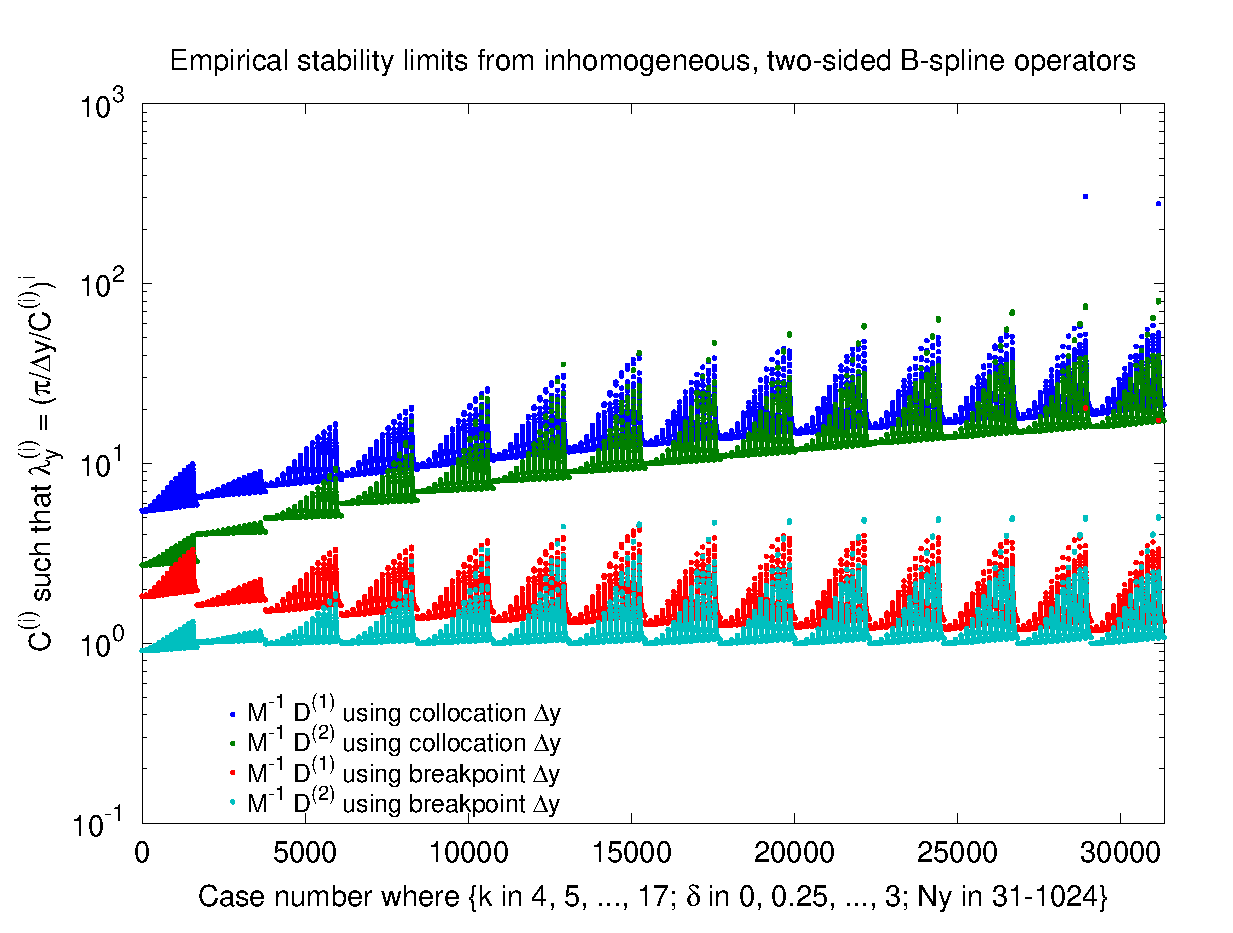
\includegraphics[width=0.85\textwidth]{inhomogeneity2}
  \\
  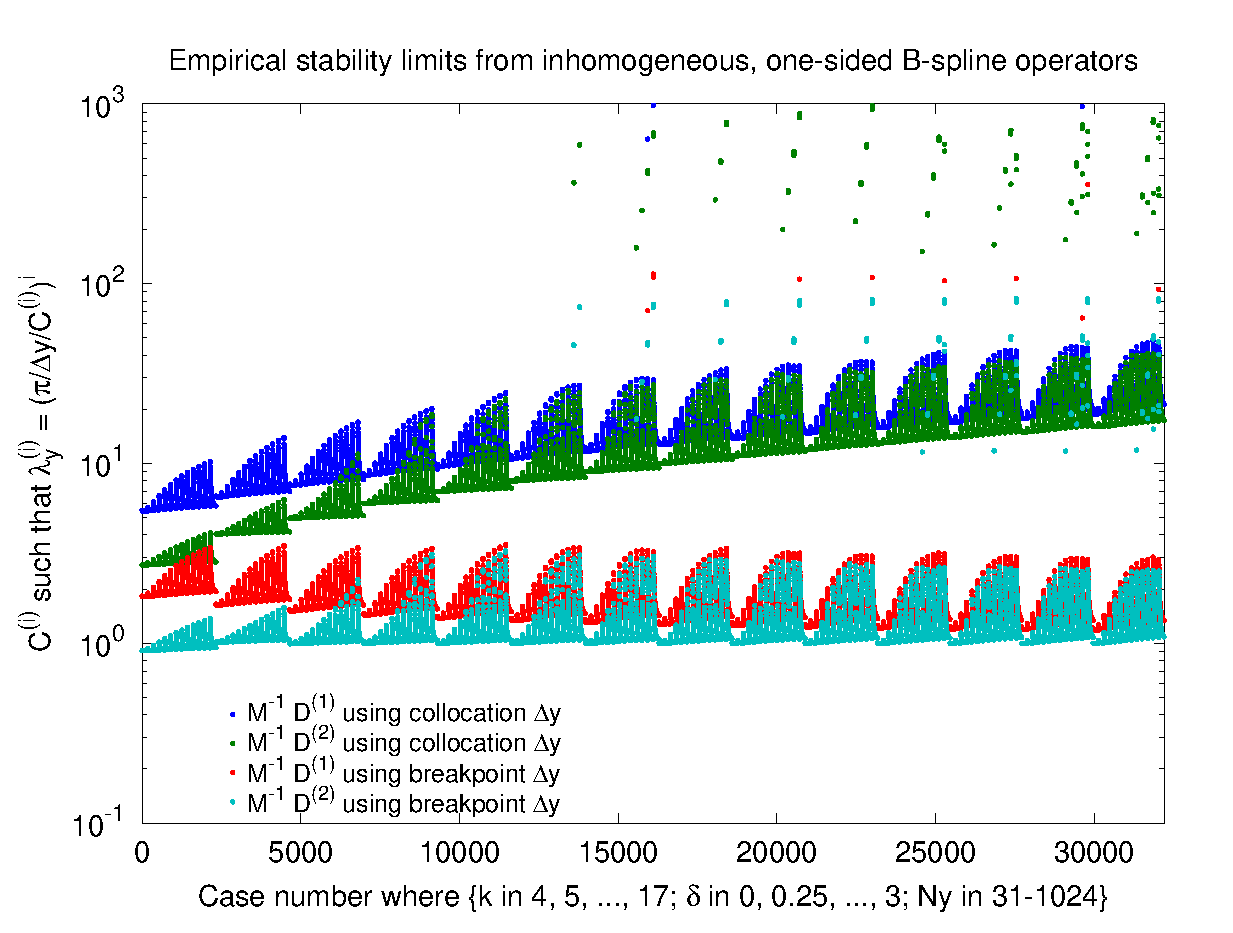
\includegraphics[width=0.85\textwidth]{inhomogeneity1}
  \\
  \caption{
  Exact values of $C^{(1)}$ and $C^{(2)}$ computed per
  equations~\eqref{eq:lambda1deltay} and~\eqref{eq:lambda2deltay} for roughly
  32,500 combinations of $k$, $\delta$, and $N_y$.  Above, two-sided stretching
  was performed on breakpoints per~\eqref{eq:htstretch2}.  Below, one-sided
  stretching was performed per~\eqref{eq:htstretch1}.  In both figures, the
  leftmost four ``triangles'' correspond to $k=4$ while $\delta$ was varied
  slowly and $N_y$ varied quickly.  Moving rightward, the next ``triangles''
  are for $k=5$, then $k=6$, etc.  Notice the logarithmic vertical axis.
  \label{fig:inhomogeneity}
  }
\end{figure}

Using actual eigenvalue magnitudes
$\lambda^{(1)}=\lambda^{(1)}_y\!\left(k,\delta,N_y\right)$ and
$\lambda^{(2)}=\lambda^{(2)}_y\!\left(k,\delta,N_y\right)$ from a large
collection of discrete operators, we computed exact results for $C^{(1)}$ and
$C^{(2)}$.  The results are shown in \autoref{fig:inhomogeneity}.  The
minimum grid spacing $\Delta{}y$ was measured using either adjacent breakpoints
or adjacent collocation points to permit a comparison.  Considering only
breakpoint-based results for $k=8$, one can see how \citet{Venugopal2003}
probably chose $C^{(1)}=4$ and $C^{(2)}=1$ as discussed in
\autoref{sec:convectivestability} and \autoref{sec:diffusivestability}.
However, it is striking just how non-universal those choices happen to be.
Evidently, neither a breakpoint-based nor a collocation point-based $\Delta{}y$
inherently captures the maximum eigenvalue magnitudes as $k$, $\delta$, and
$N_y$ vary--- some nonlinear combination of the complete set of grid parameters
is necessary.

Hereafter, unlike \citeauthor{Guarini1998}, \citeauthor{Kwok2002}, and
\citeauthor{Venugopal2003} we take $\Delta{}y$ to be the spacing between
adjacent \emph{collocation points}.  Performing Levenberg--Marquardt nonlinear
regression against the vast majority of the empirical data in
\autoref{fig:inhomogeneity} shows good agreement with curve fits like the
following
\begin{align}
  \label{eq:Cfit}
  C_\text{approx}^{(i)}\!\left(k,\delta,N_y\right)
  &\approx
    a k
  + b \hat\delta
  + \frac{c}{\sqrt{k}}
  + k^{d + e \hat\delta} \left(
        1 + \left(\frac{f k}{N_y - k + 1}\right)^{g k + h \hat\delta}
    \right)
  ,
  &
  \hat\delta &= \left(1+\delta\right)^i \tanh \delta
  .
\end{align}
The data from ``nearly spectral'' discrete operators, defined as when $N_y \leq
5 k$, proved difficult to fit and was omitted.  Such cases look like outliers
in \autoref{fig:inhomogeneity} and are not operationally important as
Suzerain is not run in production using a spectral wall-normal basis.  When
using two-sided stretching per~\eqref{eq:htstretch2}, one collection of
constants $a$--$i$ permits fitting the retained $C^{(1)}$ observations for
$k=5$ through $11$ to within relative errors of [-2.55\%, 1.76\%].  Another
collection permits fitting retained $C^{(2)}$ observations to within [-11.3\%,
17.1\%].  While those results are encouraging for the generality of the chosen
functional forms, they are less than satisfactory for production use.  More
precise, $k$-specific, coefficients for both two- and one-sided stretching
appear in \autoref{tab:C1fit} and \autoref{tab:C2fit}.

Unfortunately, using either $C_\text{approx}^{(1)}$ or $C_\text{approx}^{(2)}$
directly proves to be overly aggressive as measured using a collection of
contrived test problems known \emph{a priori} to be either convectively- or
diffusively limited.  Scaling these a by single safety factor is problematic as no
unique value allowed pushing up against both criteria simultaneously.  Against
the same test problems, however, using approximations like the square root of
$C_\text{approx}^{(i)}$ did permit using a uniform safety factor across a
variety of test conditions.

In summary, Suzerain takes nearly the square root of a conservative estimate of
$C_\text{approx}^{(i)}$.  That is, the code computes
\begin{align}
  C^{(1)} &= \left(
      \frac{C_\text{approx}^{(1)}}
           {1 - \text{(negative relative error percentage)}/100}
  \right)^{33/64}
\\
  C^{(2)} &= \left(
      \frac{C_\text{approx}^{(2)}}
           {1 - \text{(negative relative error percentage)}/100}
  \right)^{27/64}
\end{align}
where the fit-specific, negative-valued lower error bounds appear in
\autoref{tab:C1fit} and \autoref{tab:C2fit}.  Adjusting to the empirical fits'
lower bounds delivers slightly conservative $\lambda_y^{(i)}$ estimates.  These
values of $C^{(i)}$ are plugged into equations~\eqref{eq:lambda1deltay}
and~\eqref{eq:lambda2deltay} with those results feeding into
equations~\eqref{eq:convectivestability} and~\eqref{eq:diffusivestability}.
Safety factors like 0.70--0.75 are appropriate with these estimates whenever
$N_y > 5k$.

\begin{table}
\centering
\caption{
    B-spline order-specific curve fits for estimating $C_\text{approx}^{(1)}$
    via equation~\eqref{eq:Cfit} when $\Delta{}y$ is the minimum distance
    between \emph{collocation points}.  The upper half is for two-sided
    stretching $f_2$ per~\eqref{eq:htstretch2} while the bottom half is for
    one-sided stretching $f_1$ per~\eqref{eq:htstretch1}.
}
\label{tab:C1fit}
\renewcommand{\arraystretch}{1.40}   % Adds whitespace between rows
\begin{tabular}{r|ccccccccc|c@{ -- }c@{\%}}
 $k$ & $a$ & $b$ & $c$ & $d$ & $e$ & $f$ & $g$ & $h$ & $i$
     & \multicolumn{2}{c}{relative error}
\\ \hline
%%%%%%%%%%
% TWOSIDED
%%%%%%%%%%
5--11
&  $\frac{            5054}{            4549}$
& -$\frac{            3953}{           12175}$
&  $\frac{            4321}{            5893}$
& -$\frac{            5839}{            8805}$
&  $\frac{            3121}{            7385}$
&  $\frac{          235081}{            5659}$
&  $\frac{             399}{           13421}$
&  $\frac{            2795}{            8687}$
&  $\frac{            3548}{            7037}$
&  -2.55 &  1.76
\\
4
&  $\frac{            8753}{            6138}$
&  $\frac{             184}{            3513}$
& -$\frac{            3868}{            6327}$
& -$\frac{           22756}{            5215}$
&  $\frac{           19435}{           28258}$
&  $\frac{       152882005}{            9731}$
&  $\frac{            1605}{           12298}$
&  $\frac{             814}{            5783}$
&  $\frac{            7755}{           19621}$
&  -1.52 &  0.46
\\
5
& -$\frac{          182723}{            7970}$
&  $\frac{             121}{            6080}$
& -$\frac{         7061095}{           23119}$
&  $\frac{          115483}{           33477}$
&  $\frac{               1}{            5560}$
&  $\frac{             197}{            3683}$
&  $\frac{             761}{            2741}$
& -$\frac{            2307}{            6251}$
&  $\frac{            1845}{            5548}$
&  -1.12 &  0.53
\\
6
&  $\frac{            8193}{            7183}$
&  $\frac{              74}{            7487}$
&  $\frac{           10787}{            6960}$
& -$\frac{           12529}{            6209}$
&  $\frac{            3196}{            4771}$
&  $\frac{         4441318}{           12819}$
&  $\frac{             932}{           12135}$
&  $\frac{            3915}{           17923}$
&  $\frac{             870}{            2123}$
&  -1.39 &  1.14
\\
7
&  $\frac{            9063}{            5683}$
&  $\frac{             291}{            6739}$
& -$\frac{           26786}{            3839}$
& -$\frac{            2757}{            1352}$
&  $\frac{            2959}{            4613}$
&  $\frac{         2666741}{            4919}$
&  $\frac{             507}{            6947}$
&  $\frac{             498}{            2627}$
&  $\frac{            3572}{            8791}$
&  -1.50 &  1.12
\\
8
&  $\frac{           20956}{           18111}$
&  $\frac{              73}{            3043}$
&  $\frac{            3316}{            4207}$
& -$\frac{           17945}{           10877}$
&  $\frac{            6659}{           11166}$
&  $\frac{         2564433}{            9169}$
&  $\frac{             658}{           10813}$
&  $\frac{            2725}{           12594}$
&  $\frac{            1181}{            2847}$
&  -1.48 &  1.18
\\
9
&  $\frac{            4351}{            3996}$
&  $\frac{             204}{            4093}$
&  $\frac{           13726}{            5957}$
& -$\frac{           19388}{           12047}$
&  $\frac{           10397}{           18003}$
&  $\frac{         1200048}{            3823}$
&  $\frac{             246}{            4289}$
&  $\frac{            1395}{            6839}$
&  $\frac{            4244}{           10183}$
&  -1.54 &  1.09
\\
10
&  $\frac{            3174}{            3221}$
&  $\frac{             340}{            4047}$
&  $\frac{          435835}{           78898}$
& -$\frac{           24457}{           14830}$
&  $\frac{            3057}{            5416}$
&  $\frac{         5464428}{           12505}$
&  $\frac{             166}{            3013}$
&  $\frac{             679}{            3691}$
&  $\frac{            2669}{            6422}$
&  -1.59 &  1.11
\\
11
&  $\frac{            6141}{            6356}$
&  $\frac{             513}{            5051}$
&  $\frac{           35557}{            5371}$
& -$\frac{            5359}{            3384}$
&  $\frac{            6824}{           12279}$
&  $\frac{         3628675}{            8504}$
&  $\frac{            1012}{           19681}$
&  $\frac{             363}{            2008}$
&  $\frac{            1873}{            4520}$
&  -1.56 &  0.94
\\
12
&  $\frac{            9953}{            8604}$
&  $\frac{             521}{            4751}$
& -$\frac{            2623}{            3140}$
& -$\frac{           12011}{            8190}$
&  $\frac{            9067}{           16522}$
&  $\frac{         1947584}{            5723}$
&  $\frac{             141}{            2959}$
&  $\frac{            1231}{            6652}$
&  $\frac{            8479}{           20445}$
&  -1.58 &  1.12
\\
13
&  $\frac{            6428}{            6247}$
&  $\frac{              28}{             239}$
&  $\frac{           28437}{            6178}$
& -$\frac{           13912}{           10071}$
&  $\frac{            2717}{            5125}$
&  $\frac{         3512083}{           11082}$
&  $\frac{             542}{           12275}$
&  $\frac{             701}{            3776}$
&  $\frac{            7291}{           17441}$
&  -1.58 &  1.08
\\
14
&  $\frac{           18221}{           17050}$
&  $\frac{             573}{            3767}$
&  $\frac{           37351}{           13944}$
& -$\frac{           12384}{            8881}$
&  $\frac{            2238}{            4193}$
&  $\frac{         3701821}{           10597}$
&  $\frac{             231}{            5389}$
&  $\frac{            2953}{           16836}$
&  $\frac{            3950}{            9507}$
&  -1.59 &  1.10
\\
15
&  $\frac{            9251}{            9369}$
&  $\frac{            1001}{            5400}$
&  $\frac{         1033331}{          141480}$
& -$\frac{           13367}{            9358}$
&  $\frac{            7583}{           14554}$
&  $\frac{         2662722}{            5819}$
&  $\frac{             392}{            9519}$
&  $\frac{             555}{            3394}$
&  $\frac{            2181}{            5234}$
&  -1.56 &  1.01
\\
16
&  $\frac{            8003}{            8200}$
&  $\frac{            2503}{           12108}$
&  $\frac{          263686}{           31457}$
& -$\frac{            5713}{            4107}$
&  $\frac{            4803}{            9290}$
&  $\frac{         8189082}{           18419}$
&  $\frac{              93}{            2371}$
&  $\frac{            1663}{           10299}$
&  $\frac{            2945}{            7073}$
&  -1.56 &  1.08
\\
17
&  $\frac{           10594}{            8835}$
&  $\frac{            2615}{           11361}$
& -$\frac{           38602}{            5641}$
& -$\frac{            3464}{            2537}$
&  $\frac{            3372}{            6575}$
&  $\frac{         4481119}{           10024}$
&  $\frac{             355}{            9469}$
&  $\frac{             811}{            5107}$
&  $\frac{            1129}{            2714}$
&  -1.53 &  0.97
\\ \hline
%%%%%%%%%%
% ONESIDED
%%%%%%%%%%
5--11
&  $\frac{           12101}{           11060}$
& -$\frac{           16426}{           49749}$
&  $\frac{            4524}{           12157}$
& -$\frac{            4083}{            8722}$
&  $\frac{            4648}{           11133}$
&  $\frac{          645696}{           14887}$
&  $\frac{             117}{            4057}$
&  $\frac{            3436}{            8883}$
&  $\frac{            2329}{            6500}$
&  -2.80 &  2.67
\\
4
&  $\frac{            4129}{            3316}$
&  $\frac{            1052}{           13345}$
&  $\frac{            5769}{            7262}$
& -$\frac{           29140}{            6539}$
&  $\frac{            3051}{            5753}$
&  $\frac{       271951060}{            6969}$
&  $\frac{            3691}{           26472}$
&  $\frac{             458}{            3255}$
&  $\frac{            3944}{           13269}$
&  -2.65 &  1.39
\\
5
&  $\frac{            3747}{            2863}$
&  $\frac{             722}{            6223}$
& -$\frac{            3064}{           13069}$
& -$\frac{           43215}{           13954}$
&  $\frac{            4867}{            8717}$
&  $\frac{        54938146}{           12669}$
&  $\frac{             607}{            5225}$
&  $\frac{             863}{            5306}$
&  $\frac{            1663}{            5196}$
&  -2.73 &  1.43
\\
6
&  $\frac{             793}{             577}$
&  $\frac{            2234}{           16675}$
& -$\frac{           12137}{            6441}$
& -$\frac{           19450}{            5421}$
&  $\frac{            8944}{           17333}$
&  $\frac{       201430625}{            6661}$
&  $\frac{             799}{            7654}$
&  $\frac{            1290}{            9821}$
&  $\frac{             974}{            3283}$
&  -3.00 &  1.48
\\
7
&  $\frac{           10401}{            9794}$
&  $\frac{            1356}{            8845}$
&  $\frac{           30469}{           10756}$
& -$\frac{           11151}{            3473}$
&  $\frac{            3321}{            7345}$
&  $\frac{      1029376385}{           36246}$
&  $\frac{             377}{            4242}$
&  $\frac{            1838}{           13631}$
&  $\frac{            2446}{            8123}$
&  -2.88 &  1.50
\\
8
&  $\frac{           13867}{           11300}$
&  $\frac{            1847}{           10004}$
& -$\frac{             899}{            1084}$
& -$\frac{           24247}{            8311}$
&  $\frac{            2025}{            4691}$
&  $\frac{       208465759}{            9898}$
&  $\frac{            1195}{           15107}$
&  $\frac{             131}{             957}$
&  $\frac{            3041}{            9933}$
&  -2.90 &  1.47
\\
9
&  $\frac{           11292}{           11417}$
&  $\frac{            2667}{           12475}$
&  $\frac{           71783}{           14593}$
& -$\frac{           23753}{            8884}$
&  $\frac{           15279}{           38327}$
&  $\frac{       170388497}{           10015}$
&  $\frac{             913}{           12919}$
&  $\frac{            2803}{           19841}$
&  $\frac{           16957}{           54130}$
&  -2.87 &  1.41
\\
10
&  $\frac{            4941}{            9610}$
&  $\frac{             830}{            3611}$
&  $\frac{          279834}{           13813}$
& -$\frac{            4892}{            2245}$
&  $\frac{            1823}{            4351}$
&  $\frac{        11323441}{            2063}$
&  $\frac{             366}{            5827}$
&  $\frac{            1918}{           12879}$
&  $\frac{            2981}{            9362}$
&  -2.83 &  1.42
\\
11
&  $\frac{           12725}{           12639}$
&  $\frac{            1233}{            4685}$
&  $\frac{           29103}{            5882}$
& -$\frac{           17641}{            7391}$
&  $\frac{             812}{            2251}$
&  $\frac{        93817310}{            6013}$
&  $\frac{             575}{            9852}$
&  $\frac{            1238}{            8665}$
&  $\frac{            2801}{            8822}$
&  -2.79 &  1.32
\\
12
&  $\frac{            5215}{            5156}$
&  $\frac{            1009}{            3470}$
&  $\frac{           77977}{           15613}$
& -$\frac{           29719}{           12774}$
&  $\frac{            3890}{           10879}$
&  $\frac{        75236231}{            4566}$
&  $\frac{             579}{           10655}$
&  $\frac{            3977}{           28471}$
&  $\frac{            2948}{            9301}$
&  -2.86 &  1.36
\\
13
&  $\frac{           16753}{           16972}$
&  $\frac{             794}{            2485}$
&  $\frac{          100717}{           15948}$
& -$\frac{           34434}{           15637}$
&  $\frac{            2493}{            7441}$
&  $\frac{        61372987}{            4090}$
&  $\frac{             479}{            9560}$
&  $\frac{             451}{            3156}$
&  $\frac{            1286}{            3991}$
&  -2.82 &  1.34
\\
14
&  $\frac{            9761}{            9871}$
&  $\frac{            1461}{            4217}$
&  $\frac{             281}{              43}$
& -$\frac{           33703}{           15770}$
&  $\frac{            6378}{           19271}$
&  $\frac{       170777218}{           11389}$
&  $\frac{             543}{           11569}$
&  $\frac{            1880}{           13293}$
&  $\frac{            4685}{           14541}$
&  -2.82 &  1.33
\\
15
&  $\frac{            7329}{            7286}$
&  $\frac{            2281}{            6042}$
&  $\frac{           48733}{            8398}$
& -$\frac{            8421}{            4222}$
&  $\frac{            1839}{            6014}$
&  $\frac{        87107021}{            7039}$
&  $\frac{            1578}{           36371}$
&  $\frac{            1153}{            7805}$
&  $\frac{            1189}{            3613}$
&  -2.72 &  1.29
\\
16
&  $\frac{            7733}{            8163}$
&  $\frac{            3533}{            8665}$
&  $\frac{          121822}{           12527}$
& -$\frac{            6932}{            3573}$
&  $\frac{            2407}{            8036}$
&  $\frac{        57224710}{            4651}$
&  $\frac{             286}{            6989}$
&  $\frac{             377}{            2558}$
&  $\frac{            4584}{           13895}$
&  -2.72 &  1.29
\\
17
&  $\frac{           10349}{            9079}$
&  $\frac{            4121}{            9390}$
& -$\frac{           49628}{           15233}$
& -$\frac{           16811}{            8933}$
&  $\frac{            1143}{            3880}$
&  $\frac{       103494425}{            8753}$
&  $\frac{            1589}{           41049}$
&  $\frac{             817}{            5544}$
&  $\frac{            2196}{            6637}$
&  -2.66 &  1.24
\\ \hline
\end{tabular}
\end{table}

\begin{table}
\centering
\caption{
    B-spline order-specific curve fits for estimating $C_\text{approx}^{(2)}$
    via equation~\eqref{eq:Cfit} when $\Delta{}y$ is the minimum distance
    between \emph{collocation points}.  The upper half is for two-sided
    stretching $f_2$ per~\eqref{eq:htstretch2} while the bottom half is for
    one-sided stretching $f_1$ per~\eqref{eq:htstretch1}.
}
\label{tab:C2fit}
\renewcommand{\arraystretch}{1.40}   % Adds whitespace between rows
\begin{tabular}{r|ccccccccc|c@{ -- }c@{\%}}
 $k$ & $a$ & $b$ & $c$ & $d$ & $e$ & $f$ & $g$ & $h$ & $i$
     & \multicolumn{2}{c}{relative error}
\\ \hline
%%%%%%%%%%
% TWOSIDED
%%%%%%%%%%
5--11
&  $\frac{            5958}{            6049}$
&  $\frac{             334}{            5909}$
& -$\frac{           14563}{            5926}$
& -$\frac{           35330}{           11929}$
&  $\frac{            1554}{            3265}$
&  $\frac{         4042664}{            8379}$
&  $\frac{             887}{            9011}$
&  $\frac{            2243}{           13757}$
&  $\frac{            1066}{            1585}$
&  -11.30 &  17.11
\\
4
& -$\frac{          132683}{            8121}$
& -$\frac{               8}{            7617}$
& -$\frac{         1156372}{            9759}$
&  $\frac{           78080}{           22333}$
&  $\frac{               2}{           10139}$
&  $\frac{              83}{            5144}$
&  $\frac{             911}{            2744}$
& -$\frac{            4791}{           13862}$
&  $\frac{            1479}{            4412}$
&  -1.86 &  1.81
\\
5
& -$\frac{           96752}{           19419}$
&  $\frac{              27}{           10108}$
& -$\frac{          360604}{            4723}$
&  $\frac{           24551}{            9533}$
&  $\frac{               1}{            5309}$
&  $\frac{             277}{            4330}$
&  $\frac{           13424}{           46671}$
& -$\frac{            3888}{           10265}$
&  $\frac{            1289}{            3770}$
&  -0.50 &  0.32
\\
6
&  $\frac{            2635}{            8541}$
& -$\frac{             299}{           15112}$
&  $\frac{          174058}{           24237}$
& -$\frac{           17342}{           13001}$
&  $\frac{            2894}{           10471}$
&  $\frac{          291982}{            9057}$
&  $\frac{              68}{           17203}$
&  $\frac{            5579}{           13080}$
&  $\frac{            6911}{            9355}$
&  -1.51 &  2.62
\\
7
&  $\frac{            7358}{           11623}$
& -$\frac{             120}{            6169}$
&  $\frac{           82091}{           23515}$
& -$\frac{           10147}{            9621}$
&  $\frac{            2735}{           11778}$
&  $\frac{          212175}{            7154}$
&  $\frac{              10}{            6231}$
&  $\frac{           10354}{           24479}$
&  $\frac{            2416}{            3043}$
&  -1.70 &  3.97
\\
8
&  $\frac{            4751}{            5346}$
&  $\frac{            2143}{           18802}$
& -$\frac{           46259}{           19493}$
& -$\frac{            4506}{            9193}$
&  $\frac{               4}{            6951}$
&  $\frac{           49249}{            1482}$
& -$\frac{              24}{            8359}$
&  $\frac{             959}{            3662}$
&  $\frac{            9327}{            7114}$
&  -4.50 &  6.86
\\
9
&  $\frac{           17841}{           19519}$
&  $\frac{             553}{            8538}$
& -$\frac{           20719}{            8083}$
& -$\frac{            3783}{            7057}$
&  $\frac{             856}{           10529}$
&  $\frac{          121124}{            5101}$
& -$\frac{             115}{           30303}$
&  $\frac{            2467}{            7116}$
&  $\frac{            4707}{            4139}$
&  -3.68 &  7.17
\\
10
&  $\frac{           20122}{            5145}$
& -$\frac{               5}{            6272}$
& -$\frac{         1003532}{           10415}$
& -$\frac{           11287}{           15030}$
&  $\frac{            3429}{           17696}$
&  $\frac{          258125}{            9817}$
&  $\frac{               7}{            7694}$
&  $\frac{            4286}{            9151}$
&  $\frac{            8126}{            9217}$
&  -5.97 &  8.01
\\
11
&  $\frac{           32624}{           11799}$
&  $\frac{              23}{            3905}$
& -$\frac{          466211}{            6855}$
& -$\frac{           14065}{           10992}$
&  $\frac{            4693}{           11010}$
&  $\frac{          335615}{            7641}$
&  $\frac{             187}{            7994}$
&  $\frac{            4512}{            8461}$
&  $\frac{            1469}{            2419}$
&  -6.09 &  6.61
\\
12
&  $\frac{           21510}{           19531}$
&  $\frac{             407}{            3029}$
& -$\frac{           40991}{            5317}$
& -$\frac{           34333}{           13993}$
&  $\frac{            7253}{            9181}$
&  $\frac{         1291629}{            5929}$
&  $\frac{             217}{            3456}$
&  $\frac{            2659}{            8092}$
&  $\frac{            4103}{            9334}$
&  -6.88 &  6.21
\\
13
&  $\frac{            3889}{            5285}$
&  $\frac{            2389}{           15117}$
&  $\frac{           52947}{            6029}$
& -$\frac{           17456}{            5339}$
&  $\frac{            4061}{            4625}$
&  $\frac{        11135709}{            8452}$
&  $\frac{             488}{            7087}$
&  $\frac{            1474}{            6209}$
&  $\frac{             383}{             987}$
&  -6.88 &  5.89
\\
14
&  $\frac{           13010}{           10487}$
&  $\frac{            1375}{           10628}$
& -$\frac{          201367}{           12385}$
& -$\frac{           24232}{            6743}$
&  $\frac{           11512}{           10801}$
&  $\frac{         6297203}{            2487}$
&  $\frac{             428}{            6171}$
&  $\frac{             648}{            3823}$
&  $\frac{            4064}{           11831}$
&  -6.54 &  5.79
\\
15
&  $\frac{           25912}{           21893}$
&  $\frac{            1831}{           16699}$
& -$\frac{           58570}{            4063}$
& -$\frac{           14377}{            4017}$
&  $\frac{           18889}{           18281}$
&  $\frac{        16561349}{            4390}$
&  $\frac{             272}{            4179}$
&  $\frac{             367}{            2451}$
&  $\frac{             919}{            2686}$
&  -6.57 &  5.36
\\
16
&  $\frac{            3826}{            5191}$
&  $\frac{             800}{           13057}$
&  $\frac{          213790}{           16397}$
& -$\frac{           16873}{            4447}$
&  $\frac{           10559}{            9248}$
&  $\frac{        84802177}{           11958}$
&  $\frac{             607}{            9491}$
&  $\frac{            1313}{           14052}$
&  $\frac{            2667}{            8263}$
&  -6.11 &  5.04
\\
17
&  $\frac{            6127}{            6960}$
& -$\frac{             163}{            9791}$
&  $\frac{           22545}{            4961}$
& -$\frac{          115738}{           31923}$
&  $\frac{           10232}{           10879}$
&  $\frac{       167869433}{           10467}$
&  $\frac{             439}{            8114}$
&  $\frac{           10720}{           81537}$
&  $\frac{            3302}{           10275}$
&  -5.35 &  4.96
\\ \hline
%%%%%%%%%%
% ONESIDED
%%%%%%%%%%
5--11
&  $\frac{           10951}{           10966}$
&  $\frac{             692}{           17487}$
& -$\frac{           58794}{           21577}$
& -$\frac{           12439}{            4860}$
&  $\frac{            1536}{            1951}$
&  $\frac{         1826729}{            9846}$
&  $\frac{             854}{            8115}$
&  $\frac{            1731}{            7739}$
&  $\frac{            2360}{            5791}$
&  -23.87 &  19.78
\\
4
& -$\frac{           37181}{            3006}$
& -$\frac{              35}{           19004}$
& -$\frac{         1709799}{           12403}$
&  $\frac{           11429}{            3303}$
&  $\frac{               1}{            4633}$
&  $\frac{             207}{            9529}$
&  $\frac{            8025}{           25267}$
& -$\frac{            1792}{            5289}$
&  $\frac{            1579}{            6332}$
&  -2.73 &  2.66
\\
5
&  $\frac{            6843}{            7364}$
& -$\frac{             113}{            5126}$
& -$\frac{           19508}{           11693}$
& -$\frac{           15410}{            9853}$
&  $\frac{            2215}{            5596}$
&  $\frac{          199827}{            5060}$
&  $\frac{             117}{            5482}$
&  $\frac{            3886}{            7977}$
&  $\frac{            3618}{            7763}$
&  -0.63 &  1.38
\\
6
&  $\frac{            1309}{            1894}$
&  $\frac{             472}{            6839}$
&  $\frac{           10796}{           10079}$
& -$\frac{           13268}{           14331}$
&  $\frac{            1942}{           14501}$
&  $\frac{          169657}{            5987}$
&  $\frac{               2}{            3287}$
&  $\frac{            1786}{            3447}$
&  $\frac{            9664}{           13071}$
&  -3.14 &  5.22
\\
7
&  $\frac{           62991}{           64619}$
&  $\frac{           10271}{           61625}$
& -$\frac{          146725}{           39021}$
& -$\frac{            6349}{           10362}$
&  $\frac{              23}{            3440}$
&  $\frac{           26371}{             794}$
& -$\frac{              17}{           10006}$
&  $\frac{             798}{            1681}$
&  $\frac{           13080}{           14621}$
&  -4.53 &  9.31
\\
8
&  $\frac{            5701}{            6404}$
&  $\frac{             543}{           10115}$
& -$\frac{           15926}{           10845}$
& -$\frac{            9214}{           11799}$
&  $\frac{            1960}{            8807}$
&  $\frac{          759503}{           31646}$
&  $\frac{               9}{            4685}$
&  $\frac{            3636}{            5393}$
&  $\frac{            5996}{            8919}$
&  -5.10 &  7.39
\\
9
&  $\frac{           57103}{           12153}$
&  $\frac{             349}{            6313}$
& -$\frac{          292899}{            2840}$
& -$\frac{           15197}{           10802}$
&  $\frac{            3317}{            6840}$
&  $\frac{         6115361}{          140104}$
&  $\frac{             431}{            8216}$
&  $\frac{            7073}{           12325}$
&  $\frac{           10286}{           21381}$
&  -6.57 &  7.12
\\
10
&  $\frac{            4753}{            6483}$
&  $\frac{             215}{            1719}$
&  $\frac{           32327}{            6251}$
& -$\frac{            8563}{            4452}$
&  $\frac{            1981}{            2831}$
&  $\frac{         1180287}{           14438}$
&  $\frac{             599}{            7682}$
&  $\frac{            1695}{            4003}$
&  $\frac{            3259}{            8267}$
&  -8.44 &  6.56
\\
11
&  $\frac{            3058}{            4871}$
&  $\frac{            2994}{           14713}$
&  $\frac{           34703}{            3382}$
& -$\frac{           15557}{            4053}$
&  $\frac{            6541}{            5144}$
&  $\frac{         5024384}{            5503}$
&  $\frac{            2720}{           22829}$
&  $\frac{             961}{           20910}$
&  $\frac{            2347}{            7629}$
&  -6.87 &  7.13
\\
12
&  $\frac{           12242}{           10351}$
&  $\frac{             785}{            5066}$
& -$\frac{          108847}{            9907}$
& -$\frac{           38407}{            8945}$
&  $\frac{            8189}{            5423}$
&  $\frac{        54739986}{           21557}$
&  $\frac{            1903}{           16894}$
& -$\frac{             381}{            7330}$
&  $\frac{            6661}{           24933}$
&  -7.21 &  7.11
\\
13
&  $\frac{           24826}{           20307}$
&  $\frac{            4749}{           40912}$
& -$\frac{          170233}{           12219}$
& -$\frac{            4785}{            1084}$
&  $\frac{           16494}{           11557}$
&  $\frac{       720241352}{          105099}$
&  $\frac{            2930}{           29579}$
& -$\frac{             807}{           19174}$
&  $\frac{            2725}{           10439}$
&  -7.16 &  6.65
\\
14
&  $\frac{           13245}{           12827}$
&  $\frac{             163}{            5022}$
& -$\frac{           25753}{            4855}$
& -$\frac{          176237}{           37876}$
&  $\frac{           21379}{           17208}$
&  $\frac{       315490949}{            7639}$
&  $\frac{            4100}{           49413}$
&  $\frac{               2}{            4983}$
&  $\frac{            1942}{            7671}$
&  -6.65 &  6.31
\\
15
&  $\frac{            5358}{            5287}$
& -$\frac{             142}{           11949}$
& -$\frac{           16365}{            3631}$
& -$\frac{          173358}{           39355}$
&  $\frac{           10908}{           10097}$
&  $\frac{       529204799}{            8657}$
&  $\frac{             119}{            1628}$
&  $\frac{             216}{            7747}$
&  $\frac{            1637}{            6397}$
&  -6.47 &  5.75
\\
16
&  $\frac{            8995}{            9151}$
& -$\frac{             367}{            3056}$
& -$\frac{           13906}{            5041}$
& -$\frac{           40441}{           10087}$
&  $\frac{            4335}{            4703}$
&  $\frac{       366898466}{            4633}$
&  $\frac{             324}{            5153}$
&  $\frac{             440}{            8139}$
&  $\frac{            1633}{            6441}$
&  -5.99 &  5.43
\\
17
&  $\frac{           19825}{           20211}$
& -$\frac{            3148}{           12971}$
& -$\frac{            7791}{            2918}$
& -$\frac{           27739}{            8000}$
&  $\frac{            4651}{            6107}$
&  $\frac{       516527143}{            8065}$
&  $\frac{             321}{            5962}$
&  $\frac{            1049}{           12527}$
&  $\frac{            1391}{            5436}$
&  -5.04 &  5.04
\\ \hline
\end{tabular}
\end{table}

\chapter{Numerical considerations}

Here we take the complete mathematical model from \autoref{sec:derivation}
and put it into the form which Suzerain will compute per
\autoref{sec:discretization}.  Though less clean in appearance, this section's
equations will better reflect the spectral implementation details used in
Suzerain than those given in earlier sections.

\section{Convective derivative operator form}

The conservative form of the convective derivative operator,
$\nabla\cdot\left(u\otimes{}\rho{}u\right)$, is used instead of the
skew-symmetric form, $\frac{1}{2}u\cdot\nabla{}\rho{}u +
\frac{1}{2}\nabla\cdot{}u\otimes{}\rho{}u$.  The former is simpler to compute,
retains the conservative nature of the equations, and behaves comparably to the
latter in the incompressible case when aliasing errors are
removed~\citep{Zang1991Rotation}.  This choice may need to be revisited as the
wall-normal direction is not dealiased.

\section{State variable selection}
\label{state_variable_selection}

Nondimensional density $\rho$, momentum $m=\rho{}u$, and total energy
$e=\rho{}E$ are used as the state variables within the computations.  Though it
eliminates division and potentially allows for fully dealiased calculations,
specific density $\sigma=1/\rho$ is not used because it would require a
nonconservative mass equation.  When rewritten using the state variables the
equations in \autoref{nondim_equations} become
\begin{subequations}
\begin{align}
  \label{eq:state_continuity}
  \frac{\partial}{\partial{}t}\rho{}
&=
  - \nabla\cdot{}m
  + \Ssd_{\rho{}}
  \\
  \label{eq:state_momentum}
  \frac{\partial}{\partial{}t}m
&=
  - \nabla\cdot\left(\frac{m}{\rho}\otimes{}m\right)
  - \frac{1}{\Mach^{2}} \nabla{} p
  + \frac{1}{\Reynolds} \nabla\cdot\tau
  + f
  + \Ssd_{\rho{} u}
  \\
  \label{eq:state_energy}
  \frac{\partial}{\partial{}t} e
&=
  - \nabla\cdot{}\left(e + p\right)\frac{m}{\rho}
  + \frac{1}{\Reynolds\,\Prandtl\,\left( \gamma - 1 \right)}
    \nabla\cdot\mu\nabla{} T
  + \frac{\Mach^{2}}{\Reynolds} \nabla\cdot\tau{}\frac{m}{\rho}
  + \Mach^{2} f \cdot{} \frac{m}{\rho}
  + q_{b}
  + \Ssd_{\rho{} E}
\intertext{
  where the non-state quantities are fixed by
}
  \label{eq:state_pressure}
  p &= \left(\gamma-1\right) \left( e - \Mach^{2}\frac{m^2}{2\rho} \right)
  \\ \displaybreak[0]
  \label{eq:state_temperature}
  T &= \gamma{} \frac{p}{\rho}
  \\ \displaybreak[0]
  \label{eq:state_viscosity}
  \mu &= T^{\beta}
  \\ \displaybreak[0]
  \label{eq:state_secondviscosity}
  \lambda &= \left(\alpha- \frac{2}{3}\right) \mu
  \\ \displaybreak[0]
  \label{eq:state_viscousstress}
  \tau &= 2 \mu \symmetricpart{\nabla{}\frac{m}{\rho}}
        + \lambda\left(\nabla\cdot{}\frac{m}{\rho}\right) I
\end{align}
\end{subequations}
and the notation $\symmetricpart{A}=\frac{1}{2}\left(A+\trans{A}\right)$ has
been employed.

\section{Communications overhead}
\label{sec:commoverhead}

As detailed in \autoref{sec:combineddiscretization}, time advancement
occurs in wave space but nonlinear terms must be computed in physical space.
The communications and computation cost required to convert state data from
wave space to physical space or vice versa is very high.  Consequently, the
transformation back and forth happens only once per time integration substep.

\section{Velocity derivative expansions}
\label{velocity_derivative_expansions}

Because Suzerain transforms to and from physical space only once per substep,
derived quantity derivatives must be computable using only state derivatives.
Reasonable smoothness assumptions followed by expansion permit expressing
velocity derivatives as combination of state quantity derivatives:
\begin{subequations}
\begin{align}
  \nabla\cdot\frac{m}{\rho}
  &=
  \rho^{-1}\left[ \nabla\cdot{}m - \rho^{-1}m\cdot\nabla\rho \right]
\\
  \nabla{}\frac{m}{\rho}
  &=
  \rho^{-1}\left[ \nabla{}m - \rho^{-1}{m}\otimes\nabla\rho  \right]
\\
  \symmetricpart{\nabla\frac{m}{\rho}}
  &=
  \rho^{-1}\left[
      \symmetricpart{\nabla{}m}
    - \symmetricpart{\rho^{-1}m\otimes\nabla\rho}
  \right]
\\
  \Delta\frac{m}{\rho}
  &=
 \rho^{-1}\left[
      \Delta{}m
    + \rho^{-1}\left[
          \left(
              2\rho^{-1}\left(\nabla\rho\right)^{2}
            - \Delta\rho
          \right) {m}
        - 2 \left(\nabla{}m\right)\nabla\rho
      \right]
 \right]
\\
  \nabla\nabla\cdot\frac{m}{\rho}
  &=
  \rho^{-1}\left[
        \nabla\nabla\cdot{}m
      + \rho^{-1}\left[
            \left(2\rho^{-1}\nabla\rho\cdot{}m-\nabla\cdot{}m\right)\nabla\rho
          - \left(\nabla\nabla\rho\right)m
          - \trans{\nabla{}m}\nabla\rho
        \right]
  \right]
\\
  \nabla\cdot\left(\frac{m}{\rho}\otimes{}m\right)
  &=
  \rho^{-1}\left[
      \left(\nabla{}m\right)m
      + \left(\nabla\cdot{}m - \rho^{-1}m\cdot\nabla\rho\right)m
  \right]
\end{align}
\begin{align}
  \nabla\times\nabla\times\frac{m}{\rho}
  &=
  \rho^{-1}\left[
        \nabla\times\nabla\times{}{m}
      + \rho^{-1} \left[
            \left(2\nabla{}m - \trans{\nabla{}m} \right) \nabla\rho
          + \left(\Delta\rho - 2 \rho^{-1} \left(\nabla\rho\right)^2 \right) m
        \right.
  \right.
\\ % continued...
  &\qquad\qquad\qquad\qquad\qquad
  \left.
      \left.
          - \left(\nabla\nabla\rho \right) m
          + \left(2\rho^{-1}\nabla\rho\cdot{}m-\nabla\cdot{}m\right)\nabla\rho
      \right]
  \right]
\end{align}
\end{subequations}

Note several relationships amongst the information appearing in such
derivatives:
\begin{align}\label{eq:relationships}
  \Delta\rho
  &=
  \trace\left( \nabla\nabla\rho \right)
&
  \nabla\cdot{}m
  &=
  \trace\left(\nabla{}m\right)
  =
  \trace\symmetricpart{\nabla\frac{m}{\rho}}
\end{align}

\section{Separation of first and second derivative operators}
\label{sec:separate_first_second_deriv}

Unlike a Fourier basis, for B-splines the repeated application of a discrete
first derivative operator gives a result that differs significantly from
applying a discrete second derivative operator.  In particular, repeated first
differentiation severely abates high frequency modes
\citep[see][figures~2--3]{Kwok2001}.

Second differentiation enters equations~\eqref{eq:state_continuity},
\eqref{eq:state_momentum}, and~\eqref{eq:state_energy} through the terms
$\nabla\cdot\tau$, $\nabla\cdot\tau\frac{m}{\rho}$, and
$\nabla\cdot\mu\nabla{}T$.  We wish to compute these terms in a way that keeps
first and second derivative applications wholly separate.  Doing so will help
ensure that these three terms have the most physically correct diffusive impact
on high frequency content at a given spatial resolution.  These results will
also be used in the course of developing our implicit diffusive treatment.

Expanding the three mixed order, nonlinear terms and using the symmetry of
$\tau$:
\begin{align}
\label{eq:nabla_cdot_tau_expansion}
  \nabla\cdot\tau
  &=
    2 \symmetricpart{\nabla\frac{m}{\rho}}\nabla\mu
  + \mu \Delta\frac{m}{\rho}
  + \left(\mu+\lambda\right)\nabla\nabla\cdot\frac{m}{\rho}
  + \left(\nabla\cdot\frac{m}{\rho}\right)\nabla\lambda
\\
\label{eq:nabla_cdot_tau_u_expansion}
  \nabla\cdot\tau{}\frac{m}{\rho}
  &=
    \frac{m}{\rho}\cdot\left(\nabla\cdot\tau\right)
  + \trace\left( \trans{\tau}\nabla\frac{m}{\rho} \right)
\\
  \nabla\cdot\mu\nabla{}T \label{eq:mu_delta_T}
  &=
    \nabla\mu\cdot\nabla{}T
  + \mu \Delta{}T
\end{align}
One may also write
\begin{align}\label{eq:nabla_cdot_tau_expansion_alt}
  \nabla\cdot\tau
  &=
    2 \symmetricpart{\nabla\frac{m}{\rho}}\nabla\mu
  + \left(2\mu+\lambda\right) \Delta\frac{m}{\rho}
  + \left(\mu+\lambda\right)\nabla\times\nabla\times\frac{m}{\rho}
  + \left(\nabla\cdot\frac{m}{\rho}\right)\nabla\lambda
\end{align}
which highlights the isotropic diffusion of velocity within the viscous terms.

Many of the above term contains non-state derivatives which are found to be
\begin{align}
  \nabla{}p &= (\gamma-1)\left[
        \nabla{}e + \frac{\Mach^{2}}{\rho} \left[
            \frac{m^{2}}{2\rho} \nabla\rho
          - \trans{\nabla{}m}m
        \right]
  \right]
\\
  \nabla{}T &= \frac{\gamma}{\rho}
               \left[ \nabla{}p - \frac{p}{\rho}\nabla\rho \right]
             = \rho^{-1}\left( \gamma\nabla{}p - T\nabla\rho \right)
\\
  \nabla\mu &= \beta{}T^{\beta-1}\nabla{}T
\\
  \nabla\lambda &= \left(\alpha-\frac{2}{3}\right)\nabla\mu
\\
  \Delta{}p
  &=
  \left(\gamma-1\right)\left[
      \Delta{}e
      - \frac{\Mach^{2}}{\rho}\left[
            \trace\left( \trans{\nabla{}m}\nabla{}m \right)
          + m\cdot\Delta{}m
\right.\right. \notag\\ &\qquad\qquad\qquad\qquad \left.\left. % LINE BREAK
        {}- \rho^{-1}\left[
                2\trans{\nabla{}m}m\cdot\nabla{}\rho
              + \frac{1}{2} m^2 \Delta\rho
              - \rho^{-1} m^2 \left(\nabla\rho\right)^{2}
          \right]
      \right]
  \right]
\\
  \Delta{}T
  &=
  \gamma\rho^{-1}\left[
        \Delta{}p
      - \rho^{-1}\left[
            p\Delta{}\rho
          + 2\nabla{}\rho\cdot\left( \nabla{}p - \rho^{-1}p\nabla\rho \right)
      \right]
  \right]
\end{align}

Though we could have found these expressions for only the wall-normal
direction, writing them for the complete $\nabla$ operator allows reusing them
later.

\section{Implications of a fully explicit treatment}

Though our time advance allows an implicit linear term and our Fourier basis
permits repeated first differentiation, it is useful to examine the
communication costs for a purely explicit implementation.  In this context, all
terms within equations~\eqref{eq:state_continuity}, \eqref{eq:state_momentum},
and~\eqref{eq:state_energy} are formed by $\tilde{N}$ in physical space.
Further, derivatives of different orders are never mixed.  The only linear solve
required uses a wavenumber-independent factorization of the mass matrix $M$.

Using the information in \autoref{velocity_derivative_expansions}
and \autoref{sec:separate_first_second_deriv} we tabulate in
\autoref{tab:nofirstderivnonlinearcost} the specific state variable
derivatives necessary to compute each mixed-derivative nonlinear term and all
of its contributions.  From this table and the equations appearing in
\autoref{state_variable_selection}, a fully explicit timestepping approach
could compute a single substep at the cost of converting 33 scalar fields from
wave space to physical space, forming 5 scalars representing the right hand
sides of equations~\eqref{eq:state_continuity}--\eqref{eq:state_energy}, and
converting 5 scalar fields back to wave space.

While not nearly as efficient as an IMEX treatment due
to~\eqref{eq:convectivestability} and~\eqref{eq:diffusivestability}, in
conjunction with Venugopal's wall-normal modification to the convective
stability, a fully explicit treatment does allow slow progress to be made on
small problems.

%%%%%%%%%%%%%%%%%%%%%%%%%%%%%%%%%%%%%%%%%%%%%%%%%%%%%%%%%%%%%%%%%%%%%%%%%%%%%%
%%%%%%%%%%%%%%%%%%%%%%%%%%%%%%%%%%%%%%%%%%%%%%%%%%%%%%%%%%%%%%%%%%%%%%%%%%%%%%
\begin{table}[p]
\centering
\caption{
    State variable derivatives and the relative computational cost required to
    completely compute quantities in physical space without using repeated
    first derivative applications.  A check (\checkmark) indicates that a
    quantity is required to compute the given term.  A dot ($\cdot$) indicates
    the quantity is required but it can be computed from other required
    quantities.  Costs are given relative to the cost of transforming a single
    scalar field from wave space to physical space and do not include floating
    point operations. The total cost for each term is found in the rightmost
    column. Slow growth forcing does not impact this analysis.
}
\label{tab:nofirstderivnonlinearcost}
\renewcommand{\arraystretch}{1.40}   % Adds whitespace between rows
\newcommand{\cm}{\checkmark}         % For brevity in the table details
\newcommand{\cd}{\ensuremath{\cdot}} % For brevity in the table details
\begin{tabular}{r|cccc|cccccc|ccc|r}
% 001 & 002 & 003 & 004 & 005 & 006 & 007 & 008 & 009 & 011 & 012 & 013 & 014
&   1 &   3 &   1 &   6 &   3 &   1 &   6 &   9 &   3 &   3 &   1 &   3 &   1
\\
& $\rho$                                              % 01
& $\nabla\rho$                                        % 02
& $\Delta\rho$                                        % 03
& $\nabla\nabla\rho$                                  % 04
& $m$                                                 % 05
& $\nabla\cdot{}m$                                    % 06
& $\symmetricpart{\nabla{}m}$                         % 07
& $\nabla{}m$                                         % 08
& $\Delta{}m$                                         % 09
& $\nabla\nabla\cdot{}m$                              % 11
& $e$                                                 % 12
& $\nabla{}e$                                         % 13
& $\Delta{}e$                                         % 14
\\ \hline
$\nabla\cdot\frac{m}{\rho}$
% 001 & 002 & 003 & 004 & 005 & 006 & 007 & 008 & 009 & 011 & 012 & 013 & 014
& \cm & \cm &     &     & \cm & \cm &     &     &     &     &     &     &
& 8 \\
$\nabla\frac{m}{\rho}$
% 001 & 002 & 003 & 004 & 005 & 006 & 007 & 008 & 009 & 011 & 012 & 013 & 014
& \cm & \cm &     &     & \cm &     &     & \cm &     &     &     &     &
& 16 \\
$\symmetricpart{\nabla\frac{m}{\rho}}$
% 001 & 002 & 003 & 004 & 005 & 006 & 007 & 008 & 009 & 011 & 012 & 013 & 014
& \cm & \cm &     &     & \cm &     & \cm &     &     &     &     &     &
& 13 \\
$\Delta\frac{m}{\rho}$
% 001 & 002 & 003 & 004 & 005 & 006 & 007 & 008 & 009 & 011 & 012 & 013 & 014
& \cm & \cm & \cm &     & \cm &     &     & \cm & \cm &     &     &     &
& 20 \\
$\nabla\nabla\cdot\frac{m}{\rho}$
% 001 & 002 & 003 & 004 & 005 & 006 & 007 & 008 & 009 & 011 & 012 & 013 & 014
& \cm & \cm &     & \cm & \cm & \cd &     & \cm &     & \cm &     &     &
& 25 \\[1.5em]
$p$, $T$, $\mu$, $\lambda$
% 001 & 002 & 003 & 004 & 005 & 006 & 007 & 008 & 009 & 011 & 012 & 013 & 014
& \cm &     &     &     & \cm &     &     &     &     &     & \cm &     &
& 5 \\
$\nabla{}p$, $\nabla{}T$, $\nabla\mu$, $\nabla\lambda$
% 001 & 002 & 003 & 004 & 005 & 006 & 007 & 008 & 009 & 011 & 012 & 013 & 014
& \cm & \cm &     &     & \cm &     &     & \cm &     &     & \cm & \cm &
& 20 \\
$\Delta{}p$
% 001 & 002 & 003 & 004 & 005 & 006 & 007 & 008 & 009 & 011 & 012 & 013 & 014
& \cm & \cm & \cm &     & \cm &     &     & \cm & \cm &     &     &     & \cm
& 21 \\
$\Delta{}T$
% 001 & 002 & 003 & 004 & 005 & 006 & 007 & 008 & 009 & 011 & 012 & 013 & 014
& \cm & \cm & \cm &     & \cm &     &     & \cm & \cm &     & \cm & \cm & \cm
& 25 \\[1.5em]
$\tau$
% 001 & 002 & 003 & 004 & 005 & 006 & 007 & 008 & 009 & 011 & 012 & 013 & 014
& \cm & \cm &     &     & \cm & \cd & \cm &     &     &     & \cm &     &
& 14 \\[1.5em]
$\symmetricpart{\nabla\frac{m}{\rho}} \nabla\mu$
% 001 & 002 & 003 & 004 & 005 & 006 & 007 & 008 & 009 & 011 & 012 & 013 & 014
& \cm & \cm &     &     & \cm &     & \cd & \cm &     &     & \cm & \cm &
& 20 \\
$\mu\Delta\frac{m}{\rho}$
% 001 & 002 & 003 & 004 & 005 & 006 & 007 & 008 & 009 & 011 & 012 & 013 & 014
& \cm & \cm & \cm &     & \cm &     &     & \cm & \cm &     & \cm &     &
& 21 \\
$\left(\mu+\lambda\right)\nabla\nabla\cdot\frac{m}{\rho}$
% 001 & 002 & 003 & 004 & 005 & 006 & 007 & 008 & 009 & 011 & 012 & 013 & 014
& \cm & \cm &     & \cm & \cm & \cd &     & \cm &     & \cm & \cm &     &
& 26 \\
$\left(\nabla\cdot\frac{m}{\rho}\right)\nabla\lambda$
% 001 & 002 & 003 & 004 & 005 & 006 & 007 & 008 & 009 & 011 & 012 & 013 & 014
& \cm & \cm &     &     & \cm & \cd &     & \cm &     &     & \cm & \cm &
& 20 \\
$\nabla\cdot\tau$
% 001 & 002 & 003 & 004 & 005 & 006 & 007 & 008 & 009 & 011 & 012 & 013 & 014
& \cm & \cm & \cd & \cm & \cm & \cd & \cd & \cm & \cm & \cm & \cm & \cm &
& 32 \\[1.5em]
$\frac{m}{\rho}\cdot\left(\nabla\cdot\tau\right)$
% 001 & 002 & 003 & 004 & 005 & 006 & 007 & 008 & 009 & 011 & 012 & 013 & 014
& \cm & \cm & \cd & \cm & \cm & \cd & \cd & \cm & \cm & \cm & \cm & \cm &
& 32 \\
$\trace\left(\trans{\tau}\nabla\frac{m}{\rho}\right)$
% 001 & 002 & 003 & 004 & 005 & 006 & 007 & 008 & 009 & 011 & 012 & 013 & 014
& \cm & \cm &     &     & \cm & \cd & \cd & \cm &     &     & \cm &     &
& 20 \\
$\nabla\cdot\tau\frac{m}{\rho}$
% 001 & 002 & 003 & 004 & 005 & 006 & 007 & 008 & 009 & 011 & 012 & 013 & 014
& \cm & \cm & \cd & \cm & \cm & \cd & \cd & \cm & \cm & \cm & \cm & \cm &
& 32 \\[1.5em]
$\nabla\mu\cdot\nabla{}T$
% 001 & 002 & 003 & 004 & 005 & 006 & 007 & 008 & 009 & 011 & 012 & 013 & 014
& \cm & \cm &     &     & \cm &     &     & \cm &     &     & \cm & \cm &
& 20 \\
$\mu\Delta{}T$
% 001 & 002 & 003 & 004 & 005 & 006 & 007 & 008 & 009 & 011 & 012 & 013 & 014
& \cm & \cm & \cm &     & \cm &     &     & \cm & \cm &     & \cm & \cm & \cm
& 25 \\
$\nabla\cdot\mu\nabla{}T$
% 001 & 002 & 003 & 004 & 005 & 006 & 007 & 008 & 009 & 011 & 012 & 013 & 014
& \cm & \cm & \cm &     & \cm &     &     & \cm & \cm &     & \cm & \cm & \cm
& 25
\end{tabular}
\end{table}
%%%%%%%%%%%%%%%%%%%%%%%%%%%%%%%%%%%%%%%%%%%%%%%%%%%%%%%%%%%%%%%%%%%%%%%%%%%%%%
%%%%%%%%%%%%%%%%%%%%%%%%%%%%%%%%%%%%%%%%%%%%%%%%%%%%%%%%%%%%%%%%%%%%%%%%%%%%%%

\section{Hybrid implicit/explicit treatment}
\label{sec:imextreatment}

\subsection{The need for linearization}

The SMR91 time scheme requires the implicit operator $\tilde{L}$ be linear in
the state variables and time-independent.  Precious little of the
Navier--Stokes operator as written in
equations~\eqref{eq:state_continuity}--\eqref{eq:state_energy} meets these
criteria.  It must be carved up by linearization about some reference state.
This approach separates each quantity into an explicitly treated nonlinear
portion plus a linear contribution that satisfies our implicit operator
restrictions.

One example is $\rho^{-1}\Delta{}m = \lessreference{\rho^{-1}}\Delta{}m +
\reference{\rho^{-1}}\Delta{}m$ where $\reference{\rho^{-1}}$ indicates the
term $\rho^{-1}$ evaluated at some reference state.  At one extreme, treating a
three-dimensional reference field is prohibitively expensive but would provide
the longest possible time steps according to~\eqref{eq:convectivestability}
and~\eqref{eq:diffusivestability}.  At the other extreme, a uniform reference
value, which should be chosen from the wall as grid spacing is smallest there,
would have the smallest runtime overhead but would provide the smallest time
step gains.  A good compromise between these extremes is to employ a
one-dimensional reference state profile across the wall-normal direction.

Implicit operator implementation details becomes more complicated when ``off
diagonal'' state derivatives are treated implicitly.  By ``off diagonal'' we
mean derivatives of conserved state appearing on equations other than their
own.  For example, the term $\nabla\cdot{}m$ in~\eqref{eq:state_continuity} or
derivatives of the wall-normal momentum appearing in the streamwise portion
of~\eqref{eq:state_momentum}.  In contrast, an ``on diagonal'' example is the
divergence of total energy appearing within~\eqref{eq:state_energy}.  Handling
off-diagonal terms implicitly is better from the perspective of taking the
largest possible time step while maintaining stability but it incurs both an
associated programming and runtime overhead.

\subsection{Linearization of viscous terms}

Because second derivatives give rise to the most restrictive eigenvalues for
timestepping, we first focus on how second order terms enter the full operator.
Nonlinear coefficients found in second order quantities from
\autoref{velocity_derivative_expansions} and
\autoref{sec:separate_first_second_deriv} will be linearized about a reference
state.

Beginning with the nonlinear linearization candidates within $\nabla\cdot\tau$
from \eqref{eq:nabla_cdot_tau_expansion}:
\begin{align}
\label{eq:linearready_delta_u}
\mu\Delta\frac{m}{\rho} &=
    2\mu\rho^{-2}\left[
          \rho^{-1}m\left(\nabla\rho\right)^{2}
        - \left(\nabla{}m\right)\nabla\rho
    \right]
\\
  &{}+ \lessreference{\mu\rho^{-1}} \Delta{}m
     - \lessreference{\mu\rho^{-2}m} \Delta\rho
\\
  &{}+ \reference{\mu\rho^{-1}} \Delta{}m
     - \reference{\mu\rho^{-2}m} \Delta\rho
\\
\label{eq:linearready_grad_div_u}
\left(\mu+\lambda\right)\nabla\nabla\cdot\frac{m}{\rho} &=
   \left(\mu+\lambda\right)\rho^{-2}\left[
       \left(2\rho^{-1}\nabla\rho\cdot{}m-\nabla\cdot{}m\right)\nabla\rho
     - \trans{\nabla{}m}\nabla\rho
   \right]
\\
  &{}+ \lessreference{\left(\mu+\lambda\right)\rho^{-1}} \nabla\nabla\cdot{}m
\\
  &{}- \nabla\nabla\rho \lessreference{\left(\mu+\lambda\right)\rho^{-2}m}
\\
  &{}+ \reference{\left(\mu+\lambda\right)\rho^{-1}} \nabla\nabla\cdot{}m
     - \nabla\nabla\rho \reference{\left(\mu+\lambda\right)\rho^{-2}m}
\intertext{
    The term~$\frac{m}{\rho}\cdot\left(\nabla\cdot\tau\right)$ from
    expansion~\eqref{eq:nabla_cdot_tau_u_expansion} contains two similar
    contributions:
}
\label{eq:linearready_umu_delta_u}
\frac{m}{\rho}\cdot\mu\Delta\frac{m}{\rho} &=
    2\mu\rho^{-3}m\cdot\left[
          \rho^{-1}m\left(\nabla\rho\right)^{2}
        - \left(\nabla{}m\right)\nabla\rho
    \right]
\\
  &{}+ \lessreference{\mu\rho^{-2}m}\cdot\Delta{}m
     - \lessreference{\mu\rho^{-3}m^2} \Delta\rho
\\
  &{}+ \reference{\mu\rho^{-2}m}\cdot\Delta{}m
     - \reference{\mu\rho^{-3}m^2}\Delta\rho
\\
\label{eq:linearready_umu_grad_div_u}
\frac{m}{\rho}\cdot\left(\mu+\lambda\right)\nabla\nabla\cdot\frac{m}{\rho} &=
   \left(\mu+\lambda\right)\rho^{-3}m\cdot\left[
       \left(2\rho^{-1}\nabla\rho\cdot{}m-\nabla\cdot{}m\right)\nabla\rho
     - \trans{\nabla{}m}\nabla\rho
   \right]
\\
  &{}+ \lessreference{\left(\mu+\lambda\right)\rho^{-2}m}\cdot\nabla\nabla\cdot{}m
\\
  &{}- \trace\left[
           \trans{\nabla\nabla\rho}
           \lessreference{\left(\mu+\lambda\right)\rho^{-3}m\otimes{}m}
       \right]
\\
  &{}+ \reference{\left(\mu+\lambda\right)\rho^{-2}m}\cdot\nabla\nabla\cdot{}m
     - \trace\left[
           \trans{\nabla\nabla\rho}
           \reference{\left(\mu+\lambda\right)\rho^{-3}m\otimes{}m}
       \right]
\end{align}
Though linearizing the latter two terms is less common, not linearizing them
while linearizing the former two technically requires introducing more terms
into the stability criteria set forth in \autoref{sec:stabilitycriteria}.  We
implicitly treat the latter two terms to unify the numerics across the momentum
and energy equations and to acquire an additional iota of stability.

Finishing with the second order temperature term from
equation~\eqref{eq:mu_delta_T} and its dependencies:
\begin{align}
\Delta{}p =
  &{}- \left(\gamma-1\right)\Mach^{2}\rho^{-1}\left[
             \trace\left(\trans{\nabla{}m}\nabla{}m\right)
           - \rho^{-1}\left[
               2\trans{\nabla{}m}m\cdot\nabla{}\rho
             - \rho^{-1} m^2 \left(\nabla\rho\right)^{2}
           \right]
       \right]
\\
  &{}+ \left(\gamma-1\right)\Delta{}e
     - \left(\gamma-1\right)\Mach^{2}\rho^{-1}m\cdot\Delta{}m
     + \frac{\gamma-1}{2}\Mach^{2}\rho^{-2}m^2 \Delta\rho
\\
\label{eq:linear_ready_delta_T}
\mu\Delta{}T =
  &{}- 2\gamma\mu\rho^{-2}\nabla\rho\cdot
       \left(\nabla{}p-\rho^{-1}p\nabla\rho\right)
     + \gamma\mu\rho^{-1}\Delta{}p
     - \gamma\mu\rho^{-2}p\Delta\rho
\\
=
  &{}- 2\gamma\mu\rho^{-2}\nabla{}\rho\cdot
       \left(\nabla{}p-\rho^{-1}p\nabla\rho\right)
\\
  &{}- \gamma\left(\gamma-1\right)\Mach^{2}\mu\rho^{-2}\left[
             \trace\left(\trans{\nabla{}m}\nabla{}m\right)
           - \rho^{-1}\left[
               2\trans{\nabla{}m}m\cdot\nabla{}\rho
             - \rho^{-1} m^2 \left(\nabla\rho\right)^{2}
           \right]
       \right]
\\
  &{}+ \gamma\left(\gamma-1\right)\lessreference{\mu\rho^{-1}}\Delta{}e
     - \gamma\left(\gamma-1\right)\Mach^{2}
       \lessreference{\mu\rho^{-2}m}\cdot\Delta{}m
\\
  &{}+ \gamma\lessreference{
           \mu\rho^{-2}\left(\left(\gamma-1\right)e-2p\right)
       } \Delta\rho
\\
  &{}+ \gamma\left(\gamma-1\right)\reference{\mu\rho^{-1}}\Delta{}e
     - \gamma\left(\gamma-1\right)\Mach^{2}
       \reference{\mu\rho^{-2}m}\cdot\Delta{}m
     + \gamma\reference{
           \mu\rho^{-2}\left(\left(\gamma-1\right)e-2p\right)
       } \Delta\rho
\end{align}
The final line of each expansion contains linearized, implicit-ready portion.
Note that an explicit-only operator is recovered if identically zero reference
values are chosen.

\subsection{Linearization of acoustic terms}

We now focus on the first order acoustic terms within the momentum and energy
equations.  In the inviscid limit of the hyperbolic Euler equations, the
pressure gives rise to the acoustic characteristics traveling at speeds
$u\pm{}a$.  Pressure is fundamentally an off-diagonal phenomenon requiring
off-diagonal implicit treatment.

\citet[page~45]{Guarini1998} treated the pressure gradient term in the
wall-normal momentum equation and the linearized pressure work term implicitly.
The pressure gradient may be linearized as
\begin{align}
  \nabla{}p &= \left(\gamma-1\right)\Mach^{2}\left(
      \frac{1}{2} \lessreference{m^{2}\rho^{-2}}\nabla\rho
    - \trans{\nabla{}m}\lessreference{\rho^{-1}m}
  \right)
\\
&+ \left(\gamma-1\right) \nabla{}e
 + \frac{\gamma-1}{2}\Mach^{2} \reference{m^{2}\rho^{-2}}\nabla\rho
 - \left(\gamma-1\right)\Mach^{2} \trans{\nabla{}m}\reference{\rho^{-1}m}
 .
\end{align}
The total energy convection and pressure work terms may be linearized as
\begin{align}
\nabla\cdot\left(e+p\right)\frac{m}{\rho} =
   &- \left(\gamma-1\right)\mbox{Ma}^{2}\rho^{-2}m\cdot \trans{\nabla{}m}m
    + \gamma\lessreference{ \rho^{-1}m }\cdot\nabla{}e
  \\
   &+ \lessreference{
        \rho^{-1}\left(e+p\right)
      } \nabla\cdot{}m
  \\
   &+ \lessreference{
        \rho^{-2}m\left(\left(\gamma-1\right)e-2p\right)
      }\cdot\nabla\rho
  \\
   &+ \gamma\reference{
        \rho^{-1}m
      }\cdot\nabla{}e
    + \reference{
        \rho^{-1}\left(e+p\right)
      }\nabla\cdot{}m
    + \reference{
        \rho^{-2}m\left(\left(\gamma-2\right)e-2p\right)
      }\cdot\nabla\rho
.
\end{align}
The two terms have been linearized together as doing so is algebraically simple
and introduces no additional state derivatives.

\subsection{Linearity of the continuity equation}
\label{sec:contconv}

If off-diagonal density and momentum derivatives are computed implicitly,
implicitly treating the convective term $-\nabla\cdot{}m$ in
equation~\eqref{eq:state_continuity} is simple.  Doing so reduces by one the
number of scalar fields needing conversion from physical space to wave space.

\subsection{Linearization of the convective terms in the momentum equation}
\label{sec:momtconv}

Once the convective terms in equations~\eqref{eq:state_continuity}
and~\eqref{eq:state_energy} and linearized viscous terms are treated
implicitly, the incremental cost to treat the convective term in
equation~\eqref{eq:state_momentum} is small.  In particular, linearizing this
term does not increase the discrete operator bandwidth.  The linearization used
is
\begin{align}
  \nabla\cdot\left(\frac{m}{\rho}\otimes{}m\right)
&=
    \left(\nabla{}m + I \nabla\cdot{}m\right)\lessreference{\rho^{-1}m}
  - \lessreference{\rho^{-1}m\otimes\rho^{-1}m}\nabla\rho
\\
 &+ \left(\nabla{}m + I \nabla\cdot{}m\right)\reference{\rho^{-1}m}
  - \reference{\rho^{-1}m\otimes\rho^{-1}m}\nabla\rho
  .
\end{align}

Two benefits arise from this additional work.  First, simulations with
supersonic velocities at sufficiently high Reynolds number are limited by
convective stability.  Implicit treatment of the linearized convective operator
allows using a time step safety factor closer to one.  This reduces the wall
time necessary to obtain converged statistics or allows finer resolution atop
fixed computing resources.

Second, having convective terms handled implicitly in all equations replaces
$u_x$, $u_y$, and $u_z$ in criterion~\eqref{eq:convectivestability} with
$\left|u_x-u_{x0}\right|$, $\left|u_y-u_{y0}\right|$, and
$\left|u_z-u_{z0}\right|$ in a manner similar to the appearance of $\nu-\nu_0$
within criterion~\eqref{eq:diffusivestability}.  While such large time steps
cannot be taken in time-accurate simulations due to the temporal damage done to
the turbulent dynamics, such time steps will greatly accelerate time-inaccurate
simulations advancing across uninteresting transients.  For example, changing
$\Reynolds$, $\Prandtl$, or $\Mach$ often causes a lengthy transient in the
bulk energy within the domain.  Time-inaccurate simulation may be used until
the bulk energy again becomes stationary.  Of course, time-accurate
calculations must then be performed until the turbulent dynamics become
stationary prior to collecting statistics.

\subsection{The implicitly treated terms}
\label{sec:implicitlytreatedterms}

Treating wall-normal acoustics implicitly requires off-diagonal coupling
between the wall-normal momentum and total energy equations.  The incremental
programming cost to further couple the streamwise and spanwise momentum
equations to the total energy equation is comparatively small.  The ability to
treat all directions implicitly for both acoustic and diffusive terms has a
higher runtime cost which should be offset by the larger time stability that
results.  Coupling the density equation reduces the communications overhead at
the expense of on-node work (see \autoref{sec:contconv}) and further
unifies the programmatic details.  Moreover, so long as the fully coupled
implicit operations can fit in cache, increasing the on-node work to take
larger time steps (e.g. \autoref{sec:momtconv}) helps to balance the high
communication overhead stemming from \autoref{sec:commoverhead}
and \autoref{sec:separate_first_second_deriv}.  Improving the computation to
communication ratio bolsters scalability.

Accordingly, Suzerain implicitly treats all terms identified as candidates
in the preceding discussion.  In the full context of
equations~\eqref{eq:state_continuity}--\eqref{eq:state_energy} these terms are
\begin{align}
  \frac{\partial}{\partial{}t} \rho{} = &-\nabla\cdot{}m
\\
  \frac{\partial}{\partial{}t} m = \dots
% \underbrace{
   &+ \overleftrightarrow{c^{u\otimes{}u}} \nabla\rho
    - \left(\nabla{}m+I\nabla\cdot{}m\right)\overrightarrow{c^u}
% }_{-\nabla\cdot\left(\frac{m}{\rho}\otimes{}m\right)}
% \underbrace{
    - \frac{\gamma-1}{2} c^{u^2} \nabla\rho
    + \left(\gamma-1\right)\trans{\nabla{}m} \overrightarrow{c^u}
    - \frac{\gamma-1}{\Mach^2}\nabla{}e
% }_{-\Mach^{-1}\nabla{}p}
\\
% \underbrace{
   &- \Reynolds^{-1} \overrightarrow{c^{\nu{}u}} \Delta\rho
    - \Reynolds^{-1} \left(\alpha+\frac{1}{3}\right) \left(\nabla\nabla\rho\right) \overrightarrow{c^{\nu{}u}}
    + \Reynolds^{-1} c^{\nu} \Delta{}m
    + \Reynolds^{-1} \left(\alpha+\frac{1}{3}\right)c^{\nu} \nabla\nabla\cdot{}m
% }_{\Reynolds^{-1}\nabla\cdot\tau}
    + \dots
\\
  \frac{\partial}{\partial{}t} e = \dots
   &- \overrightarrow{c^{e}_{\nabla\rho}} \cdot\vec{\nabla}\rho
    - c^{e}_{\nabla\cdot{}m} \nabla\cdot{}m
    - \gamma \overrightarrow{c^u}\cdot\nabla{}e
    + \frac{\gamma}{\Reynolds\Prandtl\left(\gamma-1\right)}
      c^{e}_{\Delta\rho} \Delta\rho
    - \frac{\gamma\Mach^{2}}{\Reynolds\Prandtl}
      \overrightarrow{c^{\nu{}u}}\cdot\Delta{}m
    + \frac{\gamma}{\Reynolds\Prandtl}c^{\nu}\Delta{}e
\\
% \underbrace{
   &+ \frac{\Mach^2}{\Reynolds}\left(
       - c^{\nu{}u^2}\Delta\rho
       - \left(\alpha+\frac{1}{3}\right)
         \trace\left(\trans{\nabla\nabla\rho}
                     \overleftrightarrow{c^{\nu{}u\otimes{}u}}\right)
       + \overrightarrow{c^{\nu{}u}}\cdot\Delta{}m
       + \left(\alpha+\frac{1}{3}\right)
         \overrightarrow{c^{\nu{}u}}\cdot\nabla\nabla\cdot{}m
   \right)
% }_{\Mach^2\Reynolds^{-1}\nabla\cdot\tau\frac{m}{\rho}}
       + \dots
\end{align}
where some reference values have physically motivated superscripts
\begin{align}
  \overrightarrow{c^{u}} &= \reference{\rho^{-1}m}
  = \begin{pmatrix} c^{u_x} \\ c^{u_y} \\ c^{u_z} \end{pmatrix}
&
  c^{u^2} &= \reference{m^{2}\rho^{-2}}
&
   \overleftrightarrow{c^{u\otimes{}u}}
  = \reference{\rho^{-1}m\otimes\rho^{-1}m}
  = \begin{pmatrix}
   c^{u_x u_x} & c^{u_x u_y} & c^{u_x u_z} \\
   c^{u_x u_y} & c^{u_y u_y} & c^{u_y u_z} \\
   c^{u_x u_z} & c^{u_y u_z} & c^{u_z u_z}
  \end{pmatrix}
\end{align}
\begin{align}
  c^{\nu} &= \reference{\rho^{-1}\mu}
&
  \overrightarrow{c^{\nu{}u}} &= \reference{\rho^{-2}\mu{}m}
  = \begin{pmatrix} c^{\nu{}u_x} \\ c^{\nu{}u_y} \\ c^{\nu{}u_z} \end{pmatrix}
&
  c^{\nu{}u^2} &= \reference{\rho^{-3}\mu{}m^2}
\end{align}
\begin{align}
   \overleftrightarrow{c^{\nu{}u\otimes{}u}}
  = \reference{\rho^{-3}\mu{}m\otimes{}m}
  = \begin{pmatrix}
   c^{\nu{} u_x u_x} & c^{\nu{} u_x u_y} & c^{\nu{} u_x u_z} \\
   c^{\nu{} u_x u_y} & c^{\nu{} u_y u_y} & c^{\nu{} u_y u_z} \\
   c^{\nu{} u_x u_z} & c^{\nu{} u_y u_z} & c^{\nu{} u_z u_z}
  \end{pmatrix}
\end{align}
while the remaining reference values
\begin{align}
  \overrightarrow{c^{e}_{\nabla\rho}} &= \reference{
        m\rho^{-2}\left(\left(\gamma-2\right)e-2p\right)
  }
  = \begin{pmatrix}
      c^{e_{x}}_{\nabla\rho} \\
      c^{e_{y}}_{\nabla\rho} \\
      c^{e_{z}}_{\nabla\rho}
  \end{pmatrix}
&
  c^{e}_{\nabla\cdot{}m} &= \reference{
        \rho^{-1}\left(e + p\right)
  }
&
  c^{e}_{\Delta\rho} &= \reference{
        \mu\rho^{-2}\left(\left(\gamma-1\right)e-2p\right)
  }
\end{align}
have superscripts indicating the relevant equation and
subscripts indicating the associated term.

\subsection{Discretization of the implicitly treated terms}
\label{sec:discretizationofimplicitterms}
Following Algorithm~\ref{alg:step} per \eqref{eq:spatial_discretization},
$M+\varphi{}L$ must be implemented for arbitrary $\varphi$, $k_m$, and $k_n$.
$L$ is nothing but the discrete form of the linear terms from the previous
section.  Notice for any reference values $c^{\bullet}$ left-multiplying by
the diagonal matrix
\begin{align}
  C^{\bullet} &= \begin{bmatrix}
   \left.c^{\bullet}\right|_{y=0} &        & 0 \\
                                  & \ddots &    \\
   0                              &        & \left.c^{\bullet}\right|_{y=L}
   \end{bmatrix}
\end{align}
scales linear operators in a way that accommodates wall-normal variations in
reference quantities.  For example, applying $C^{\nu}D^{(2)}$ rather than
$D^{(2)}$ scales the result at collocation point $y=y_l$ by
$\left.c^{\nu}\right|_{y=y_l}$.

Switching to a blocked matrix representation employing five scalar conserved
state fields, the complete, implicit-ready discrete operator $M+\varphi{}L$ is
shown in \autoref{fig:discreteimplicitop}.  The representation chosen
highlights how the full operator is built from discrete operators applied to
individual state fields.  Strong Dirichlet boundary conditions may be enforced
in the usual way.  Neumann boundary condition implementations are less
straightforward.  For simulations with no mean bulk velocity in the spanwise
direction, the reference coefficient matrices $C^{u_z}$ and $C^{\nu{}u_z}$ may
be treated as effectively zero.  This reduces the required linear algebra.  If
desired, the density equation and density terms in the other equations may
removed from the result in \autoref{fig:discreteimplicitop} to greatly
reduce operator assembly and factorization overhead.  Previous work by
\citet{Guarini1998} did not treat density implicitly.  Note, however, implicit
density treatment will be assumed in \autoref{sec:nonreflectingbcs}.
Finally, implicitly handling only the wall-normal directions may be
accomplished by setting $k_{m}$ and $k_{n}$ to zero.  Doing so results in a
wavenumber independent operator requiring factorization only once per substep.

\begin{sidewaysfigure}
\newcommand{\entry}[1]{}          % Provides comments for subblocks
\newcommand{\C}[2]{C^{#1}_{#2}}   % For brevity below
\newcommand{\D}[1]{D^{(#1)}}      % ditto
\newcommand{\M}{M}                % ditto
\newcommand{\g}{\gamma}           % ditto
\newcommand{\km}{k_{m}}           % ditto
\newcommand{\kn}{k_{n}}           % ditto
\newcommand{\mx}{m_{x}}           % ditto
\newcommand{\my}{m_{y}}           % ditto
\newcommand{\mz}{m_{z}}           % ditto
\newcommand{\vp}{\varphi}         % ditto
\newcommand{\subcoeff}[3]{{       % ditto
   \renewcommand{\arraystretch}{2.0}
   \begin{Bmatrix}{#1}\\{#2}\\{#3}\end{Bmatrix}
}}
\newcommand{\Ma}{\ensuremath{\mbox{\small{}Ma}}}
\renewcommand{\Pr}{\ensuremath{\mbox{\small{}Pr}}}
\renewcommand{\Re}{\ensuremath{\mbox{\small{}Re}}}
\newcommand{\ind}[1]{\textcolor{BrickRed}{#1}}  % Wavenumber independent term
\hspace{-.04\textwidth}
{\resizebox{1.08\textwidth}{!}{\begin{minipage}[c]{\textwidth}  % SCALE-TO-FIT
\begin{align*}
\ind{\bm{\vp}}
\renewcommand{\arraystretch}{9.0} % Adds whitespace between rows
\addtolength{\arraycolsep}{-.1em}
\begin{bmatrix}
% Density row
  \entry{\rho\rho}
  \subcoeff{
      \ind{\bm{\frac{1}{\vp}}} % M
  }{
  }{
  }
& \entry{\rho\mx }
  \subcoeff{
    - \ii\km
  }{
  }{
  }
& \entry{\rho\my }
  \subcoeff{
  }{
    \ind{- 1}
  }{
  }
& \entry{\rho\mz }
  \subcoeff{
    - \ii\kn
  }{
  }{
  }
& \entry{\rho{}e }
  \ind{0}
% Streamwise momentum row
\\\entry{\mx\rho }
  \subcoeff{
    \begin{pmatrix}
        \frac{1-\g}{2}\ii\km\C{u^2}{}
      + \frac{\left(\alpha+\frac{4}{3}\right)\km^2+\kn^2}{\Re}\C{\nu{}u_x}{}
      + \frac{\alpha+\frac{1}{3}}{\Re}\km\kn\C{\nu{}u_z}{}
      \\
      + \ii\km\C{u_x u_x}{}
      + \ii\kn\C{u_x u_z}{}
    \end{pmatrix}
  }{
    - \frac{\alpha+\frac{1}{3}}{\Re}\ii\km\C{\nu{}u_y}{}
    + \ind{\C{u_x u_y}{}}
  }{
    \ind{- \frac{1}{\Re}\C{\nu{}u_x}{}}
  }
& \entry{\mx\mx  }
  \subcoeff{
      \ind{\bm{\frac{1}{\vp}}} % M
    + \left(\g-3\right)\ii\km\C{u_x}{}
    - \ii\kn\C{u_z}{}
    - \frac{\left(\alpha+\frac{4}{3}\right)\km^2+\kn^2}{\Re}\C{\nu}{}
  }{
    \ind{- \C{u_y}{}}
  }{
    \ind{  \frac{1}{\Re}\C{\nu}{}}
  }
& \entry{\mx\my  }
  \subcoeff{
      \left(\g-1\right)\ii\km\C{u_y}{}
  }{
    \ind{- \C{u_x}{}}
    + \frac{\alpha+\frac{1}{3}}{\Re}\ii\km\C{\nu}{}
  }{
  }
& \entry{\mx\mz  }
  \subcoeff{
      \left(\g-1\right)\ii\km\C{u_z}{}
    - \ii\kn\C{u_x}{}
    - \frac{\alpha+\frac{1}{3}}{\Re}\km\kn\C{\nu}{}
  }{
  }{
  }
& \entry{\mx{}e  }
  \subcoeff{
      \frac{1-\g}{\Ma^2}\ii\km
  }{
  }{
  }
% Wall-normal momentum row
\\\entry{\my\rho }
  \subcoeff{
      \frac{\km^2+\kn^2}{\Re}\C{\nu{}u_y}{}
    + \ii\km\C{u_x u_y}{}
    + \ii\kn\C{u_y u_z}{}
  }{
      \ind{\frac{1-\g}{2}\C{u^2}{}}
    - \frac{\alpha+\frac{1}{3}}{\Re}\ii\left(
         \km\C{\nu{}u_x}{} + \kn\C{\nu{}u_z}{}
      \right)
    + \ind{\C{u_y u_y}{}}
  }{
    \ind{- \frac{\alpha+\frac{4}{3}}{\Re}\C{\nu{}u_y}{}}
  }
& \entry{\my\mx  }
  \subcoeff{
    - \ii\km\C{u_y}{}
  }{
      \ind{\left(\g-1\right)\C{u_x}{}}
    + \frac{\alpha+\frac{1}{3}}{\Re}\ii\km\C{\nu}{}
  }{
  }
& \entry{\my\my  }
  \subcoeff{
      \ind{\bm{\frac{1}{\vp}}} % M
    - \ii\km\C{u_x}{}
    - \ii\kn\C{u_z}{}
    - \frac{\km^2+\kn^2}{\Re}\C{\nu}{}
  }{
      \ind{\left(\g-3\right)\C{u_y}{}}
  }{
      \ind{\frac{\alpha+\frac{4}{3}}{\Re}\C{\nu}{}}
  }
& \entry{\my\mz  }
  \subcoeff{
    - \ii\kn\C{u_y}{}
  }{
      \ind{\left(\g-1\right)\C{u_z}{}}
    + \frac{\alpha+\frac{1}{3}}{\Re}\ii\kn\C{\nu}{}
  }{
  }
& \entry{\my{}e  }
  \subcoeff{
  }{
      \ind{\frac{1-\g}{\Ma^2}}
  }{
  }
% Spanwise momentum row
\\\entry{\mz\rho}
  \subcoeff{
    \begin{pmatrix}
        \frac{1-\g}{2}\ii\kn\C{u^2}{}
      + \frac{\km^2+\left(\alpha+\frac{4}{3}\right)\kn^2}{\Re}\C{\nu{}u_z}{}
      + \frac{\alpha+\frac{1}{3}}{\Re}\km\kn\C{\nu{}u_x}{}
      \\
      + \ii\km\C{u_x u_z}{}
      + \ii\kn\C{u_z u_z}{}
    \end{pmatrix}
  }{
    - \frac{\alpha+\frac{1}{3}}{\Re}\ii\kn\C{\nu{}u_y}{}
    + \ind{\C{u_y u_z}{}}
  }{
    \ind{- \frac{1}{\Re}\C{\nu{}u_z}{}}
  }
& \entry{\mz\mx }
  \subcoeff{
      \left(\g-1\right)\ii\kn\C{u_x}{}
    - \ii\km\C{u_z}{}
    - \frac{\alpha+\frac{1}{3}}{\Re}\km\kn\C{\nu}{}
  }{
  }{
  }
& \entry{\mz\my }
  \subcoeff{
      \left(\g-1\right)\ii\kn\C{u_y}{}
  }{
    \ind{- \C{u_z}{}}
    + \frac{\alpha+\frac{1}{3}}{\Re}\ii\kn\C{\nu}{}
  }{
  }
& \entry{\mz\mz }
  \subcoeff{
      \ind{\bm{\frac{1}{\vp}}} % M
    - \ii\km\C{u_x}{}
    + \left(\g-3\right)\ii\kn\C{u_z}{}
    - \frac{\km^2+\left(\alpha+\frac{4}{3}\right)\kn^2}{\Re}\C{\nu}{}
  }{
    \ind{- \C{u_y}{}}
  }{
    \ind{  \frac{1}{\Re}\C{\nu}{}}
  }
& \entry{\mz{}e }
  \subcoeff{
      \frac{1-\g}{\Ma^2}\ii\kn
  }{
  }{
  }
% Total energy row
\\\entry{e\rho  }
  \subcoeff{
    \begin{pmatrix}
      - \ii\left(\km\C{e_x}{\nabla\rho} + \kn\C{e_z}{\nabla\rho}\right)
      \\
      - \g\frac{\km^2+\kn^2}{\Re\Pr\left(\g-1\right)}\C{e}{\Delta\rho}
      + \frac{\Ma^2}{\Re}\left(\km^2+\kn^2\right)\C{\nu{}u^2}{}
      \\
      + \frac{\Ma^2}{\Re}\left(\alpha+\frac{1}{3}\right)\left(
              \km^2 \C{\nu{}u_x u_x}{}
          + 2 \km\kn\C{\nu{}u_x u_z}{}
          +   \kn^2 \C{\nu{}u_z u_z}{}
        \right)
    \end{pmatrix}
  }{
    \ind{- \C{e_y}{\nabla\rho}}
    + \frac{\Ma^2}{\Re}\left(\alpha+\frac{1}{3}\right)\left(
       - 2\ii\km\C{\nu{}u_x u_y}{}
       - 2\ii\kn\C{\nu{}u_y u_z}{}
      \right)
  }{
    \ind{
      {\frac{\g}{\Re\Pr\left(\g-1\right)}\C{e}{\Delta\rho}}
    - \frac{\Ma^2}{\Re}\C{\nu{}u^2}{}
    - \frac{\Ma^2}{\Re}\left(\alpha+\frac{1}{3}\right)\C{\nu{}u_y u_y}{}
    }
  }
& \entry{e\mx   }
  \subcoeff{
    \begin{pmatrix}
      \frac{\Ma^2}{\Re}\left[
          \left(\frac{\g}{\Pr}-\left(\alpha+\frac{4}{3}\right)\right)\km^2
        + \left(\frac{\g}{\Pr}-1                              \right)\kn^2
      \right] \C{\nu{}u_x}{}
      \\
      - \frac{\Ma^2}{\Re}\left(\alpha+\frac{1}{3}\right) \km\kn\C{\nu{}u_z}{}
      - \ii\km\C{e}{\nabla\cdot{}m}
    \end{pmatrix}
  }{
    \frac{\Ma^2}{\Re}\left(\alpha+\frac{1}{3}\right)\ii\km\C{\nu{}u_y}{}
  }{
    \ind{\frac{\Ma^2}{\Re}\left(1 - \frac{\g}{\Pr}\right)\C{\nu{}u_x}{}}
  }
& \entry{e\my   }
  \subcoeff{
    \frac{\Ma^2}{\Re}\left(\frac{\g}{\Pr} - 1\right)
    \left(\km^2+\kn^2\right)\C{\nu{}u_y}{}
  }{
    \ind{- \C{e}{\nabla\cdot{}m}}
    + \frac{\Ma^2}{\Re}\left(\alpha+\frac{1}{3}\right)\left(
          \ii\km\C{\nu{}u_x}{}
        + \ii\kn\C{\nu{}u_z}{}
      \right)
  }{
    \ind{
    \frac{\Ma^2}{\Re}\left[
      \left(\alpha+\frac{4}{3}\right) - \frac{\g}{\Pr}
    \right] \C{\nu{}u_y}{}
    }
  }
& \entry{e\mz   }
  \subcoeff{
    \begin{pmatrix}
      \frac{\Ma^2}{\Re}\left[
          \left(\frac{\g}{\Pr}-1                              \right)\km^2
        + \left(\frac{\g}{\Pr}-\left(\alpha+\frac{4}{3}\right)\right)\kn^2
      \right] \C{\nu{}u_z}{}
      \\
      - \frac{\Ma^2}{\Re}\left(\alpha+\frac{1}{3}\right) \km\kn\C{\nu{}u_x}{}
      - \ii\kn\C{e}{\nabla\cdot{}m}
    \end{pmatrix}
  }{
    \frac{\Ma^2}{\Re}\left(\alpha+\frac{1}{3}\right)\ii\kn\C{\nu{}u_y}{}
  }{
    \ind{\frac{\Ma^2}{\Re}\left(1 - \frac{\g}{\Pr}\right) \C{\nu{}u_z}{}}
  }
& \entry{ee     }
  \subcoeff{
      \ind{\bm{\frac{1}{\vp}}} % M
    - \g\ii\left(\km\C{u_x}{} + \kn\C{u_z}{}\right)
    - \frac{\g}{\Re\Pr}\left(\km^2+\kn^2\right)\C{\nu}{}
  }{
    \ind{- \g\C{u_y}{}}
  }{
    \ind{  \frac{\g}{\Re\Pr}\C{\nu}{}}
  }
\end{bmatrix}
\renewcommand{\arraystretch}{1.0}
\begin{bmatrix}
  \hat{\rho}_{\left(0,\,m,\,n\right)} \\
  \vdots \\
  \hat{\rho}_{\left(N_y-1,\,m,\,n\right)} \\
\\%
\\%
\\%
\\%
  \hat{\mx}_{\left(0,\,m,\,n\right)} \\
  \vdots \\
  \hat{\mx}_{\left(N_y-1,\,m,\,n\right)} \\
\\%
\\%
\\%
\\%
  \hat{\my}_{\left(0,\,m,\,n\right)} \\
  \vdots \\
  \hat{\my}_{\left(N_y-1,\,m,\,n\right)} \\
\\%
\\%
\\%
\\%
  \hat{\mz}_{\left(0,\,m,\,n\right)} \\
  \vdots \\
  \hat{\mz}_{\left(N_y-1,\,m,\,n\right)} \\
\\%
\\%
\\%
\\%
  \hat{e}_{\left(0,\,m,\,n\right)} \\
  \vdots \\
  \hat{e}_{\left(N_y-1,\,m,\,n\right)} \\
%
\end{bmatrix}
\end{align*}
\end{minipage}}}  % END SCALE-TO-FIT!
\vspace{2em}
\\
\caption[The discrete operator $M+\varphi{}L$ used for implicit time advance]
{
    The complete discrete operator $M+\varphi{}L$ used for implicit time advance is
    depicted.  Notice the leftmost scalar factor $\bm{\vp}$.  The $3 N_y \times
    N_y$ blocked vectors surrounded by curly braces are to be ``dotted'' against
    the blocked vector $ \trans{\begin{bmatrix} \M & \D{1} & \D{2} \end{bmatrix}} $
    to form $N_y \times N_y$ subblocks.  Each of $M$, $\D{1}$, and $\D{2}$ is a
    $N_y \times N_y$ banded matrix.  Reference quantities like $C^\nu$ are $N_y
    \times N_y$ diagonal matrices.  The complex-valued, wavenumber-dependent
    operator takes wall-normal B-spline coefficients to B-spline collocation point
    values.  A real-valued, wavenumber-independent operator is the degenerate case
    obtained by setting $\km=\kn=0$; the nonzero terms in this special circumstance
    are \ind{colored}.
}
\label{fig:discreteimplicitop}
\end{sidewaysfigure}

\subsection{Implementation of the discretized implicit operator}
\label{sec:bsmbsm}

The discretized implicit operator $M+\varphi{}L$ depicted in
\autoref{fig:discreteimplicitop} is a blocked square matrix with banded
submatrices (BSMBSM).  Matrix $A$ is said to be a BSMBSM when
\[A = \begin{pmatrix}
    B^{0,0}  & \cdots & B^{0,S-1}   \\
    \vdots    & \ddots & \vdots       \\
    B^{S-1,0} & \cdots & B^{S-1,S-1}
\end{pmatrix}\]
where every $B^{i,j}$ is an $\mathtt{n}$ by $\mathtt{n}$ banded submatrix
containing $\mathtt{kl}$ subdiagonals and $\mathtt{ku}$ superdiagonals.  In
this section we set the convention that lowercase fixed-width identifiers
indicate submatrix details while uppercase ones indicate global details for
$A$.  The structure of a BSMBSM is defined completely by the parameters
$\mathtt{S}$, $\mathtt{n}$, $\mathtt{kl}$, and $\mathtt{ku}$.  The number of
rows and columns is $\mathtt{N} = \mathtt{S}\,\mathtt{n}$.

Applying $A$ from individually contiguous, banded submatrices $B_{i,j}$ within
$A$ is both convenient and efficient.  For example, banded matrix accumulation
operations and boundary condition imposition are simple in such a storage
format.  However, using individually contiguous, banded submatrices is grossly
inefficient for solving linear equations.

With appropriate renumbering of $A$, solving linear equations can be done
efficiently.  The zero-indexed permutation vector \[q(i) =
\left(i\bmod{}S\right)n + \lfloor{}i/S\rfloor{}\] may always be used to convert
a BSMBSM into a globally banded $\mathtt{N}$ by $\mathtt{N}$ matrix with
minimum bandwidth.  More concretely, the permutation matrix $P$ uniquely
defined by vector $q$ causes $P A \trans{P}$ to have $\mathtt{KL} =
\mathtt{S}\left(\mathtt{kl}+1\right)-1$ subdiagonals and
$\mathtt{KU}=~\mathtt{S}\left(\mathtt{ku}+1\right)-1$ superdiagonals summing to
overall bandwidth $\mathtt{KL} + 1 + \mathtt{KU} = \mathtt{S}\left(\mathtt{kl}
+ \mathtt{ku} + 2\right)-1$.  The reverse permutation vector has a simple
closed form \[q^{-1}(i) = \left(i\bmod{}n\right)S + \lfloor{}i/n\rfloor{}.\]
With $A_{i,j}$ in hand, the banded renumbering may be formed using the
relationships
\begin{align}
    \label{eq:bsmbsm_renumbering}
       \left.A\right|_{i,j}
    &= \left.P A \trans{P}\right|_{q^{-1}(i),q^{-1}(j)}
    &
       \left.P A \trans{P}\right|_{i,j}
    &= \left.A\right|_{q(i),q(j)}.
\end{align}
This renumbering can be LU factorized in order $\mathtt{N}\left(\mathtt{KL} + 1
+ \mathtt{KU}\right)^2 =
\mathtt{S}\,\mathtt{n}\left(\mathtt{S}\left(\mathtt{kl} + \mathtt{ku} +
2\right)-1\right)^2$ floating point operations to find $LU = P A \trans{P}$.
Recent work has shown forthcoming ``manycore'' architectures to be efficient at
performing many such conveniently parallel
factorizations~\citep{Schulz2012Early}.  The linear equation $AX=B$, which is
equivalent to $LUPX=PB$, then has the solution \[X = A^{-1}B =
\trans{P}\left(LU\right)^{-1}PB\] where inversion has been used as a notational
convenience representing triangular back substitution.

\section{Boundary conditions}

\subsection{Isothermal walls with and without transpiration}

An isothermal boundary requires specifying a constant temperature
$T_\mathrm{w}$.  Both no-slip and transpiring walls are of interest.  The
former possess constant wall velocities $u_\mathrm{w} = v_\mathrm{w} =
w_\mathrm{w} = 0$ while the later permit nonzero-but-constant velocities.  A
transpiring wall condition is achieved by setting $v_\mathrm{w} > 0$.  One
thermodynamic quantity must be allowed to vary for such boundary conditions to
be well-posed.  Allowing $\rho$ to vary in time is simplest given our state
choices.  Assuming smoothness and combining~\eqref{eq:state_pressure}
and~\eqref{eq:state_temperature} within the total energy equation yields four
constraints:
\begin{align}
   \partial_t \left(\rho u\right)_\mathrm{w}
&= u_\mathrm{w} \partial_t \rho_\mathrm{w} + \rho_\mathrm{w} \partial_t u_\mathrm{w}
 = u_\mathrm{w} \partial_t \rho_\mathrm{w}
\\
   \partial_t \left(\rho v\right)_\mathrm{w}
&= v_\mathrm{w} \partial_t \rho_\mathrm{w} + \rho_\mathrm{w} \partial_t v_\mathrm{w}
 = v_\mathrm{w} \partial_t \rho_\mathrm{w}
\\
   \partial_t \left(\rho u\right)_\mathrm{w}
&= u_\mathrm{w} \partial_t \rho_\mathrm{w} + \rho_\mathrm{w} \partial_t u_\mathrm{w}
 = u_\mathrm{w} \partial_t \rho_\mathrm{w}
\\
   \partial_t \left(\rho E\right)_\mathrm{w}
&= E_\mathrm{w} \partial_t \rho_\mathrm{w} + \rho_\mathrm{w} \partial_t E_\mathrm{w}
 = E_\mathrm{w} \partial_t \rho_\mathrm{w}
 = \left(
     \frac{T_\mathrm{w}}{\gamma\left(\gamma-1\right)}
   + \frac{\Mach^2}{2}\left(u_\mathrm{w}^2+v_\mathrm{w}^2+w_\mathrm{w}^2\right)
   \right) \partial_{t} \rho
\end{align}
These conditions may be strongly enforced by linear implicit operators using
how B-spline basis support limits the number of nonzero coefficients at the
wall as discussed in \autoref{sec:formingoperators}.

\subsection{Nonreflecting freestream boundary conditions}
\label{sec:nonreflectingbcs}

When simulating problems on semi-infinite domains, such as flat plates,
Suzerain requires nonreflecting freestream boundary conditions.  Without these,
acoustic waves generated by the flow cannot leave the domain.   The trapped
acoustics pile up causing a non-physical partition of energy and spoiling the
simulated statistics.

Following \citet{Engquist1977Absorbing},
\citet{Giles1988Nonreflecting,Giles1990Nonreflecting} developed localized,
approximate two-dimensional, unsteady nonreflecting boundary conditions for the
Euler equations.  Giles' boundary conditions are adopted over the ``locally
one-dimensional inviscid'' relations of \citet{Poinsot1992Boundary} because
other codes with similar numerics have successfully employed Giles' conditions
for our problems of interest.  While \citet{Rowley2000Discretely} present
higher order techniques expected to perform better than Giles' approach, what
they describe is considerably more complex to implement.
\citet{Saxer1993QuasiThreeDimensional} extended the technique to three
dimensions but with a presentation aimed towards transonic axial flow
turbomachinery computations.  \citet{Guarini1998} summarizes the Cartesian
extension of Giles' approach to three spatial dimensions without reproducing
the associated analysis.  \citet{Medida2007} lucidly catalogs the intermediate
results necessary in three dimensions.  Useful test cases and sample boundary
condition behaviors are cataloged by \citet{Baum1995Accurate}.

\subsubsection{Giles' abstract approach}
\label{sec:gilesabstract}

We now review Giles' approach following Guarini's presentation with the goal of
setting notation suitable for presenting and manipulating Medida's results for
nonreflecting $x$ boundaries in three-dimensional, Cartesian coordinates.  For
complete details, especially motivations and proofs, the work of Giles, Medida,
and Guarini should be consulted in that respective order.

For the state vector
\begin{subequations}
\label{eq:eulerprim}
\begin{align}
  U &= \left\{ \rho, u, v, w, p \right\}
\end{align}
the Euler equations, using the ideal gas equation of state
\begin{align}
  \rho a^2 &= \gamma p,
\end{align}
may be written as follows:
\begin{align}
    \frac{\partial}{\partial{}t}U
+ A \frac{\partial}{\partial{}x}U
+ B \frac{\partial}{\partial{}y}U
+ C \frac{\partial}{\partial{}z}U
&= 0
\end{align}
\begin{align}
 A &= \begin{bmatrix}
        u & \rho     & 0 & 0 & 0              \\
        0 & u        & 0 & 0 & \frac{1}{\rho} \\
        0 & 0        & u & 0 & 0              \\
        0 & 0        & 0 & u & 0              \\
        0 & \gamma p & 0 & 0 & u              \\
       \end{bmatrix}
&
 B &= \begin{bmatrix}
        v & 0 & \rho     & 0 & 0              \\
        0 & v & 0        & 0 & 0              \\
        0 & 0 & v        & 0 & \frac{1}{\rho} \\
        0 & 0 & 0        & v & 0              \\
        0 & 0 & \gamma p & 0 & v              \\
       \end{bmatrix}
&
 C &= \begin{bmatrix}
        w & 0 & 0 & \rho     & 0              \\
        0 & w & 0 & 0        & 0              \\
        0 & 0 & w & 0        & 0              \\
        0 & 0 & 0 & w        & \frac{1}{\rho} \\
        0 & 0 & 0 & \gamma p & w              \\
       \end{bmatrix}
\end{align}
\end{subequations}
This system of equations identically describes the behavior of an analogous
$U^*$ whenever all of
\begin{align}
\label{eq:eulerprimnondim}
U^{*} &= \left\{
  \frac{\rho}{\rho_0},
  \frac{u}{u_0},
  \frac{v}{u_0},
  \frac{w}{u_0},
  \frac{p}{\rho_0 u_0^2}
\right\}
&
t_0 &= \frac{l_0}{u_0}
&
a_0 &= u_0
\end{align}
hold.  Therefore, all dimensional results obtained for $U$ remain unchanged
in the setting of $U^*$.

Consider perturbations
\[
\delta{}U = \left\{ \delta{}\rho, \delta{}u,
\delta{}v, \delta{}w, \delta{}p \right\}
\]
taken about some steady,
uniform reference state $\bar{U}$ so that
\[
U = \bar{U} + \delta{}U.
\]
The short-time evolution of such perturbations is governed by the linearized
Euler equations
\begin{align}
\label{eq:dimeulerperturb}
               \frac{\partial}{\partial{}t}\delta{}U
+ \bar{A} \frac{\partial}{\partial{}x}\delta{}U
+ \bar{B} \frac{\partial}{\partial{}y}\delta{}U
+ \bar{C} \frac{\partial}{\partial{}z}\delta{}U
&= 0
\end{align}
where matrices $\bar{A}$, $\bar{B}$, and $\bar{C}$ are evaluated
at $\bar{U}$.  This linearized system satisfies the prerequisites for
Giles' analysis.  Assuming a solution of the form
\begin{align}
  \delta{}U &= e^{\ii\left(
    k_x x + k_y y + k_z z - \omega t
  \right)}
  \delta\hat{U}^R
\end{align}
and substituting into the linearized equations reduces the equations to
\begin{align}
\label{eq:dimeulerreduced}
  \ii\left( - \omega I
            + k_x \bar{A}
            + k_y \bar{B}
            + k_z \bar{C}
  \right)
  \delta\hat{U}^R &= 0
\end{align}
which has nontrivial solutions only if the so-called dispersion relation
\begin{align}
  \det \left( - \omega I
              + k_x \bar{A}
              + k_y \bar{B}
              + k_z \bar{C}
       \right) &= 0
\end{align}
holds.  Defining $\lambda_x = k_x/\omega$, $\lambda_y = k_y/\omega$, and
$\lambda_z/\omega$, the dispersion relation may be equivalently expressed as
\begin{align}
\label{eq:dimeulerdisp}
  \det \left( - I
              + \lambda_x \bar{A}
              + \lambda_y \bar{B}
              + \lambda_z \bar{C}
       \right) &= 0
  .
\end{align}
Assuming $\bar{A}$ is invertible and applying
$-\left(\ii\omega{}\bar{A}\right)^{-1}$ to
equation~\eqref{eq:dimeulerreduced}, one finds an eigenvalue problem in
$\lambda_x$
\begin{align}
  \left(   \bar{A}^{-1}
         - \lambda_x I
         - \lambda_y \bar{A}^{-1} \bar{B}
         - \lambda_z \bar{A}^{-1} \bar{C}
  \right) \delta\hat{U}^R = 0
\end{align}
where $\delta\hat{U}^R$ is the eigenvector and a solution to the right null
space problem.  The signs of the associated eigenvalues, determined using the
magnitude of $\bar{u}$ relative to $\bar{a}$, are required to determine how
many characteristics are entering or exiting through the boundary.  The left
null space problem
\begin{align}
\label{eq:dimeulereigenprob}
  V^{L}
  \left(   \bar{A}^{-1}
         - \lambda_x I
         - \lambda_y \bar{A}^{-1} \bar{B}
         - \lambda_z \bar{A}^{-1} \bar{C}
  \right) &= 0
\end{align}
naturally gives rise to the associated left null vector $V^L$.  Giles,
following Engquist and Majda, used several orthogonality properties to build
the exact, nonreflecting boundary conditions
\begin{align}
\label{eq:dimeulerexact}
  V_n^L \delta{}U &= 0
\end{align}
for each $V_n^L = V^L\!\left(k_{x_n}\right)$ corresponding to \textit{either
incoming or outgoing waves}.  This exact condition is approximated using a
Taylor series in $\lambda_y$ and $\lambda_z$ for reasons of computational
tractability.  Truncating the series is equivalent to assuming waves have a
small angle of incidence to the boundary.  To first order,
\begin{align}
  \left.V_n^L\right|_{\lambda_y,\lambda_z=0}
  \delta{}U
  +
  \lambda_y
  \left.\frac{dV_n^L}{d\lambda_y}\right|_{\lambda_y,\lambda_z=0}
  \delta{}U
  +
  \lambda_z
  \left.\frac{dV_n^L}{d\lambda_z}\right|_{\lambda_y,\lambda_z=0}
  \delta{}U
  &\approx 0
  .
\end{align}
As noted by \citet{Engquist1977Absorbing} and later expounded upon by
\citet{Trefethen1986Wellposedness}, only particular higher-order series
truncations of this form lead to well-posedness.  Moreover, the straightforward
application of even this first order approximation requires either
ad~hoc~\citep{Giles1988Nonreflecting,Medida2007} or
systematic~\citep{Rowley2000Discretely} modification to produce well-behaved
inflow constraints.  Multiplying through by $-\ii\omega$, Fourier transforming
in both time and space, and using that $\bar{U}$ and therefore $V_n^L$ are both
steady and uniform yields
\begin{align}
\label{eq:dimeulerapprox}
  \frac{\partial}{\partial{}t}
  V^L
  \delta{}U
  &\approx
  \frac{dV^L}{d\lambda_y}
  \frac{\partial}{\partial{}y}\delta{}U
  +
  \frac{dV^L}{d\lambda_z}
  \frac{\partial}{\partial{}z}\delta{}U
\end{align}
where the cumbersome $\lambda_y,\lambda_z=0$ and subscript $n$ are herein
and henceforth suppressed.  Inserting ${V^L}^{-1} V^L$,
\begin{align}
  \frac{\partial}{\partial{}t}
  V^L
  \delta{}U
  &\approx
  \frac{dV^L}{d\lambda_y}
  {V^L}^{-1}
  \frac{\partial}{\partial{}y}
  V^L
  \delta{}U
  +
  \frac{dV^L}{d\lambda_z}
  {V^L}^{-1}
  \frac{\partial}{\partial{}z}
  V^L
  \delta{}U
.
\end{align}
Defining characteristic variables using the action of $V^L$, viz.
\begin{align}
  \delta{}C &= V^L \delta{}U
  ,
\end{align}
allows writing a more compact form
\begin{align}
  \frac{\partial}{\partial{}t}
  \delta{}C
  &\approx
  B^G
  \frac{\partial}{\partial{}y}
  \delta{}C
  +
  C^G
  \frac{\partial}{\partial{}z}
  \delta{}C
\end{align}
employing the notation
\begin{align}
  B^G
&=
  \frac{dV^L}{d\lambda_y}
  {V^L}^{-1}
&
  C^G
&=
  \frac{dV^L}{d\lambda_z}
  {V^L}^{-1}
\end{align}
where the superscript $G$ is meant to suggest ``Giles''.

Condition \eqref{eq:dimeulerapproxchar} intermingles the constraints for
inflow and outflow conditions.  Only the incoming characteristics should be
evolved.  Which waves are incoming may be determined by comparing the magnitude
of $\bar{u}$ relative to $\bar{a}$.  Care must be taken to account for the
choices made in representing $V^L$ as and to correctly treat left versus right
boundaries.  Notationally, it will later be convenient to have a
projection
\begin{align}
\label{eq:PG}
  P^G
  &:
  \delta{C} \to \delta{C}
\end{align}
such that
\begin{align}
\label{eq:dimeulerapproxchar}
  P^G
  \frac{\partial}{\partial{}t}
  \delta{}C
  &\approx
  P^G B^G
  \frac{\partial}{\partial{}y}
  \delta{}C
  +
  P^G C^G
  \frac{\partial}{\partial{}z}
  \delta{}C
\end{align}
imposes conditions on only incoming characteristics.  In contrast, applying
\begin{align}
 I - P^G
 &:
 \delta{C} \to \delta{C}
\end{align}
recovers the outgoing characteristics not constrained by the boundary condition
For some $\bar{U}$ possessing an agreed upon relationship between $\bar{u}$ and
$\bar{a}$, specifying $V^L$, $P^G$, $B^G$, and $C^G$ concretely states a
Giles-like nonreflecting $x$ boundary condition for the Euler equations.

\subsubsection{Medida's subsonic inflow and outflow conditions}

In section 5.8 of his thesis, Medida presents two such concrete nonreflecting
boundary condition specifications for subsonic inflows and outflows where $0 <
\bar{u} < \bar{a}$.  Medida's equations~(5.78) and~(5.79) specify the
transformations to and from characteristic variables:
\begin{align}
\label{eq:dimeulerapproxmedidaproj}
  V^L &= \left[\begin{array}{ccccc}
    -\bar{a}^2 & 0                   & 0                  & 0                  & 1 \\ \noalign{\smallskip}
    0          & 0                   & \bar{\rho} \bar{a} & 0                  & 0 \\ \noalign{\smallskip}
    0          & 0                   & 0                  & \bar{\rho} \bar{a} & 0 \\ \noalign{\smallskip}
    0          & \bar{\rho} \bar{a}  & 0                  & 0                  & 1 \\ \noalign{\smallskip}
    0          & -\bar{\rho} \bar{a} & 0                  & 0                  & 1 \\ \noalign{\smallskip}
  \end{array}\right]
&
  {V^L}^{-1} &= \left[\begin{array}{ccccc}
    -\frac{1}{\bar{a}^2} & 0                            & 0                            & \frac{1}{2\bar{a}^2}          & \frac{1}{2\bar{a}^2}            \\ \noalign{\smallskip}
    0                    & 0                            & 0                            & \frac{1}{2\bar{\rho} \bar{a}} & - \frac{1}{2\bar{\rho} \bar{a}} \\ \noalign{\smallskip}
    0                    & \frac{1}{\bar{\rho} \bar{a}} & 0                            & 0                             & 0                               \\ \noalign{\smallskip}
    0                    & 0                            & \frac{1}{\bar{\rho} \bar{a}} & 0                             & 0                               \\ \noalign{\smallskip}
    0                    & 0                            & 0                            & \frac{1}{2}                   & \frac{1}{2}                     \\ \noalign{\smallskip}
  \end{array}\right]
\end{align}
For this $V^L$, the characteristics $\delta{}C$ travel at speeds
$\left[\bar{u}, \bar{u}, \bar{u}, \bar{u}+\bar{a}, \bar{u}-\bar{a}\right]$.
Direct computation shows
\[
  \det V^L = -2\bar{\rho}^3\bar{a}^5
\]
and so $V^L$ is always nonsingular for a realizable reference state.  Medida's
equations~(5.82) and~(5.83) provide one set of nonreflecting conditions for
which reflection coefficients were not reported:
\begin{align}
\label{eq:dimeulerapproxmedidaopt1}
  B^G_1 &= \left[\begin{array}{ccccc}
    0 & 0                         & 0       & 0                           & 0                         \\ \noalign{\smallskip}
    0 & \bar{v}                   & 0       & \frac{\bar{a} + \bar{u}}{2} & \frac{\bar{a}-\bar{u}}{2} \\ \noalign{\smallskip}
    0 & 0                         & \bar{v} & 0                           & 0                         \\ \noalign{\smallskip}
    0 & \frac{\bar{a}-\bar{u}}{2} & 0       & \bar{v}                     & 0                         \\ \noalign{\smallskip}
    0 & \bar{u}                   & 0       & 0                           & \bar{v}                   \\ \noalign{\smallskip}
  \end{array}\right]
&
  C^G_1 &= \left[\begin{array}{ccccc}
    0 & 0       & 0                         & 0                         & 0                         \\ \noalign{\smallskip}
    0 & \bar{w} & 0                         & 0                         & 0                         \\ \noalign{\smallskip}
    0 & 0       & \bar{w}                   & \frac{\bar{a}+\bar{u}}{2} & \frac{\bar{a}-\bar{u}}{2} \\ \noalign{\smallskip}
    0 & 0       & \frac{\bar{a}-\bar{u}}{2} & \bar{w}                   & 0                         \\ \noalign{\smallskip}
    0 & 0       & \bar{u}                   & 0                         & \bar{w}                   \\ \noalign{\smallskip}
  \end{array}\right]
\end{align}
Using the one-dimensional outward normal $n$ with value $-1$ or $1$ at a left
or right boundary, respectively,
\begin{align}
\label{eq:PGmedida}
  P^G
  &=
  \left(
  n
  \left[\begin{array}{ccccc}
    \bar{u} & 0       & 0       & 0                 & 0                 \\
    0       & \bar{u} & 0       & 0                 & 0                 \\
    0       & 0       & \bar{u} & 0                 & 0                 \\
    0       & 0       & 0       & \bar{u} + \bar{a} & 0                 \\
    0       & 0       & 0       & 0                 & \bar{u} - \bar{a} \\
  \end{array}\right]
  <
  0
  \right)
\end{align}
returns the appropriate projection operator if comparisons are deemed to
indicate 1 if true and 0 if false.

We assume, but have not verified, analysis like that presented in
\citet[\textsection{}3.7.4]{Giles1988Nonreflecting} extends to Medida's
analogous results.  At the inflow, the outgoing pressure wave produces no
reflected entropy or vorticity waves and generates a fourth-order pressure
reflection.  At the outflow, the outgoing entropy and vorticity waves produce
no reflections while the outgoing pressure wave produces a second order
reflection.  In contrast, Medida's equation~(5.84), which arises from modifying
the already-well-posed outflow condition to match the well-posed inflow
condition, provides different outflow behavior:
\begin{align}
\label{eq:dimeulerapproxmedidaopt2}
  B^G_2 &= \left[\begin{array}{ccccc}
    0 & 0                         & 0       & 0                           & 0                         \\ \noalign{\smallskip}
    0 & \bar{v}                   & 0       & \frac{\bar{a} + \bar{u}}{2} & \frac{\bar{a}-\bar{u}}{2} \\ \noalign{\smallskip}
    0 & 0                         & \bar{v} & 0                           & 0                         \\ \noalign{\smallskip}
    0 & \frac{\bar{a}-\bar{u}}{2} & 0       & \bar{v}                     & 0                         \\ \noalign{\smallskip}
    0 & \frac{\bar{a}+\bar{u}}{2} & 0       & 0                           & \bar{v}                   \\ \noalign{\smallskip}
  \end{array}\right]
&
  C^G_2 &= \left[\begin{array}{ccccc}
    0 & 0       & 0                         & 0                         & 0                         \\ \noalign{\smallskip}
    0 & \bar{w} & 0                         & 0                         & 0                         \\ \noalign{\smallskip}
    0 & 0       & \bar{w}                   & \frac{\bar{a}+\bar{u}}{2} & \frac{\bar{a}-\bar{u}}{2} \\ \noalign{\smallskip}
    0 & 0       & \frac{\bar{a}-\bar{u}}{2} & \bar{w}                   & 0                         \\ \noalign{\smallskip}
    0 & 0       & \frac{\bar{a}+\bar{u}}{2} & 0                         & \bar{w}                   \\ \noalign{\smallskip}
  \end{array}\right]
\end{align}
At an outflow, these matrices cause outgoing pressure waves to produce fourth
and first order reflections, respectively.  As Giles
notes~\citep{Giles1990Nonreflecting}, this second outflow condition is
preferable only when one knows there will be no outgoing vorticity wave.  This
should be the case for some of our problems of interest.

\subsubsection{Application to the chosen nondimensional state variables}

In section~4.3 of his thesis, \citet{Guarini1998} proved the linear
structure of the Euler equations admits a straightforward translation of Giles'
boundary conditions to another set of state variables $V$ with steady, uniform
reference state $\bar{V}$ and therefore perturbations
\begin{align}
  \label{eq:gilesperturbV}
  \delta{}V &= V - \bar{V}.
\end{align}
The corresponding coordinate transformation Jacobian matrix is
\[
   S = \frac{\partial{}U}{\partial{}V}
   .
\]
In this new setting, Guarini rewrote the exact nonreflecting
conditions~\eqref{eq:dimeulerexact} as
\begin{align}
  \left(V^L S\right) \delta{}V &= 0
\end{align}
which causes the approximate condition~\eqref{eq:dimeulerapprox} to become
\begin{align}
\label{eq:dimeulertransform}
  V^L
  S
  \frac{\partial}{\partial{}t}
  \delta{}V
  &\approx
  \frac{dV^L}{d\lambda_y}
  S
  \frac{\partial}{\partial{}y}
  \delta{}V
  +
  \frac{dV^L}{d\lambda_z}
  S
  \frac{\partial}{\partial{}z}
  \delta{}V
  .
\end{align}
Using notation from the compact representation~\eqref{eq:dimeulerapproxchar}
\begin{align}
\label{eq:dimeulertransformcharnot}
  P^G V^L S
  \frac{\partial}{\partial{}t}
  \delta{}V
  &\approx
  P^G B^G V^L S
  \frac{\partial}{\partial{}y}
  \delta{}V
  +
  P^G C^G V^L S
  \frac{\partial}{\partial{}z}
  \delta{}V
\end{align}
is the simplest form for applying Medida's $x$ boundary condition matrices to
alternative state variables.

The particular coordinate transformation Suzerain requires maps the
nondimensional primitive state $U^*$ satisfying
requirements~\eqref{eq:eulerprimnondim} to the conserved state $V^*$
nondimensionalized per \autoref{sec:nondimrefq} and \autoref{nondim_equations}:
\begin{align}
\label{eq:eulerconsnondim}
V^{*}
&= \left\{
  \frac{\rho}{\rho_0},
  \frac{\rho u}{\rho_0 u_0},
  \frac{\rho v}{\rho_0 u_0},
  \frac{\rho w}{\rho_0 u_0},
  \frac{\rho E}{\rho_0 a_0^2}
\right\}
= \left\{
    \rho^{*},
  \,\rho^{*} u^{*},
  \,\rho^{*} v^{*},
  \,\rho^{*} w^{*},
  \,\rho^{*} E^{*}
\right\}
&
a^{*} &= \frac{a}{a_0}
&
\Mach &= \frac{u_0}{a_0}
&
t_0 &= \frac{l_0}{u_0}
\end{align}
Observing several relationships between $U^*$ and $V^*$ with care to
distinguish between $u_0$ and $a_0$
\begin{align}
  \frac{\rho}{\rho_0} &= \rho^*
&
  \frac{u}{u_0} &=
  \frac{\frac{\rho{}u}{\rho_0u_0}}{\frac{\rho}{\rho_0}}
  =
  \frac{\rho^{*}u^{*}}{\rho^{*}}
&
  \frac{v}{u_0} &= \frac{\rho^{*}v^*}{\rho^*}
&
  \frac{w}{u_0} &= \frac{\rho^{*}w^*}{\rho^*}
\end{align}
\begin{align}
 \frac{p}{\rho_0 u_0^2}
&=
   \frac{\gamma-1}{\rho_0 u_0^2} \rho E
 + \frac{1-\gamma}{2 \rho_0 u_0^2 \rho}\left(
           \left(\rho{}u\right)^2
         + \left(\rho{}v\right)^2
         + \left(\rho{}w\right)^2
   \right)
=
   \frac{\gamma-1}{\Mach^2} \rho^{*} E^{*}
 + \frac{1-\gamma}{2 \rho^{*}}\left(
           \left(\rho^{*}u^{*}\right)^2
         + \left(\rho^{*}v^{*}\right)^2
         + \left(\rho^{*}w^{*}\right)^2
   \right)
\end{align}
aids computing the Jacobian matrix evaluated at some $\bar{V}^{*}$,
\begin{align}
S &= \left[\begin{array}{ccccc}
    1      % 11
  & 0      % 12
  & 0      % 13
  & 0      % 14
  & 0      % 15
  \\ \noalign{\medskip}
    - \frac{\bar{u}^*}{\bar{\rho}^*} % 21
  & \frac{1}{\bar{\rho}^*}           % 22
  & 0                                % 23
  & 0                                % 24
  & 0                                % 25
  \\ \noalign{\medskip}
    - \frac{\bar{v}^*}{\bar{\rho}^*} % 31
  & 0                                % 32
  & \frac{1}{\bar{\rho}^*}           % 33
  & 0                                % 34
  & 0                                % 35
  \\ \noalign{\medskip}
    - \frac{\bar{w}^*}{\bar{\rho}^*} % 41
  & 0                                % 42
  & 0                                % 43
  & \frac{1}{\bar{\rho}^*}           % 44
  & 0                                % 45
  \\ \noalign{\medskip}
    \frac{\gamma-1}{2}\left({\bar{u}^*}^2+{\bar{v}^*}^2+{\bar{w}^*}^2\right) % 51
  & \left(1 - \gamma\right) \bar{u}^*   % 52
  & \left(1 - \gamma\right) \bar{v}^*   % 53
  & \left(1 - \gamma\right) \bar{w}^*   % 54
  & \frac{\gamma-1}{\Mach^2}            % 55
  \\ \noalign{\medskip}
\end{array}\right]
.
\end{align}
As expected, the transformation is nonsingular for realizable fields because
\[
  \det S = \frac{\gamma-1}{\Mach^2 {\bar{\rho}^{*}}^3}.
\]
The inverse is
\begin{align}
S^{-1} &= \left[\begin{array}{ccccc}
  1                                                                       & 0                              & 0                              & 0                              & 0                        \\
  \bar{u}^{*}                                                             & \bar{\rho}^*                   & 0                              & 0                              & 0                        \\
  \bar{v}^{*}                                                             & 0                              & \bar{\rho}^*                   & 0                              & 0                        \\
  \bar{w}^{*}                                                             & 0                              & 0                              & \bar{\rho}^*                   & 0                        \\
  \frac{\Mach^2}{2}\left({\bar{u}^*}^2+{\bar{v}^*}^2+{\bar{w}^*}^2\right) & \Mach^2 \bar{\rho}^* \bar{u}^* & \Mach^2 \bar{\rho}^* \bar{v}^* & \Mach^2 \bar{\rho}^* \bar{w}^* & \frac{\Mach^2}{\gamma-1}
\end{array}\right]
.
\end{align}
Medida's matrices $V^L$, $B^G$, and $C^G$ derived for $U$ remain valid for
nondimensional $U^*$ possessing sound speed $a/u_0$.  When reusing these
matrices for $V^*$ every sound speed must be scaled by $1/\Mach$ because
\[
  \frac{\bar{a}}{u_0} = \frac{a_0 \bar{a}^*}{u_0} = \frac{\bar{a}^*}{\Mach}.
\]
The correctness of this intuitive find-and-replace operation has been verified
using \emph{Mathematica} to reproduce Medida's results in this particular
nondimensional context.

Thus far nonreflecting $x$ boundary conditions in physical space have been
presented.  Suzerain requires rotating these results to handle nonreflecting
$y$ boundaries followed by transforming the constraints into coefficient space.
Defining
\begin{align}
  x' &= z &
  y' &= x &
  z' &= y
\intertext{
induces the following relationships:
}
  u &= v' &
  v &= w' &
  w &= u'
\\
  \frac{\partial}{\partial{}x} &= \frac{\partial}{\partial{}y'} &
  \frac{\partial}{\partial{}y} &= \frac{\partial}{\partial{}z'} &
  \frac{\partial}{\partial{}z} &= \frac{\partial}{\partial{}x'}
\end{align}
The perturbed state vector entries may be reordered more conventionally by
defining $R^Y$ and $\delta{}V'$ per
\begin{align}
  \delta{}V
  &= \begin{bmatrix}
       \delta\rho     \\
       \delta\rho{}v' \\
       \delta\rho{}w' \\
       \delta\rho{}u' \\
       \delta\rho{}E  \\
     \end{bmatrix}
  = R^Y \delta{}V'
  = \begin{bmatrix}
      1 & 0 & 0 & 0 & 0 \\
      0 & 0 & 1 & 0 & 0 \\
      0 & 0 & 0 & 1 & 0 \\
      0 & 1 & 0 & 0 & 0 \\
      0 & 0 & 0 & 0 & 1 \\
    \end{bmatrix}
    \begin{bmatrix}
      \delta\rho     \\
      \delta\rho{}u' \\
      \delta\rho{}v' \\
      \delta\rho{}w' \\
      \delta\rho{}E  \\
    \end{bmatrix}
  .
\end{align}
Substituting these details into equation~\eqref{eq:dimeulertransformcharnot}
produces the desired nonreflecting $y$ boundary condition,
\begin{align}
\label{eq:dimeulertransformcharnotYwieldy}
\left.\left[
  P^G V^L S
\right]\right|_{\bar{u}=\bar{v}', \bar{v}=\bar{w}', \bar{w}=\bar{u}'}
  R^Y
  \frac{\partial}{\partial{}t}
  \delta{}V'
&\approx
\left.\left[
  P^G C^G V^L S
\right]\right|_{\bar{u}=\bar{v}', \bar{v}=\bar{w}', \bar{w}=\bar{u}'}
  R^Y
  \frac{\partial}{\partial{}x'}
  \delta{}V'
\\&+
\left.\left[
  P^G B^G V^L S
\right]\right|_{\bar{u}=\bar{v}', \bar{v}=\bar{w}', \bar{w}=\bar{u}'}
  R^Y
  \frac{\partial}{\partial{}z'}
  \delta{}V'
.
\end{align}
Suppressing the primes and matrix evaluation details makes the above result
much more wieldy,
\begin{align}
\label{eq:dimeulertransformcharnotYphys}
  \left[P^G V^L S\right]
  R^Y
  \frac{\partial}{\partial{}t}
  \delta{}V
&\approx
  \left[P^G C^G V^L S\right]
  R^Y
  \frac{\partial}{\partial{}x}
  \delta{}V
  +
  \left[P^G B^G V^L S\right]
  R^Y
  \frac{\partial}{\partial{}z}
  \delta{}V
.
\end{align}
Replacing $\delta{}V$ by $V - \bar{V}$ per~\eqref{eq:gilesperturbV} and
recalling that by assumption
$
    \frac{\partial}{\partial{}t} \bar{V}
  = \frac{\partial}{\partial{}x} \bar{V}
  = \frac{\partial}{\partial{}z} \bar{V}
  = 0
$,
\begin{align}
  \left[P^G V^L S\right]
  R^Y
  \frac{\partial}{\partial{}t}
  V
&\approx
  \left[P^G C^G V^L S\right]
  R^Y
  \frac{\partial}{\partial{}x}
  V
  +
  \left[P^G B^G V^L S\right]
  R^Y
  \frac{\partial}{\partial{}z}
  V
.
\end{align}
Transforming to Fourier space gives a linear condition almost suitable for
implicit advance per \autoref{sec:timediscretization},
\begin{align}
  \left[P^G V^L S\right]
  R^Y
  \frac{\partial}{\partial{}t}
  \hat{V}
&\approx
  \ii k_x
  \left[P^G C^G V^L S\right]
  R^Y
  \hat{V}
  +
  \ii k_z
  \left[P^G B^G V^L S\right]
  R^Y
  \hat{V}
.
\end{align}
Notice that when $k_x=k_z=0$ the relevant mean characteristics are held
constant in time.  The previous evolution equation is a pointwise condition
suitable when $\hat{V}$ contains pointwise state (e.g. collocation point
values).  When another representation is chosen for state, one should use
\begin{align}
\label{eq:dimeulertransformcharnotYwave}
  \left[P^G V^L S\right]
  R^Y
  M \frac{\partial}{\partial{}t}
  \hat{V}
&\approx
  \ii k_x
  \left[P^G C^G V^L S\right]
  R^Y
  M \hat{V}
  +
  \ii k_z
  \left[P^G B^G V^L S\right]
  R^Y
  M \hat{V}
\end{align}
where time-invariant $M$ maps state to non-state.  However, the distinction is
somewhat blurred for B-spline boundary collocation points and boundary
coefficients because the boundary value for a B-spline basis expansion is
nothing but the boundary coefficient.

While equation~\eqref{eq:dimeulertransformcharnotYwave} constrains incoming
characteristics, it does not evolve the remainder in accordance with the
interior of the simulation domain.  Returning to the time discretization of
\autoref{sec:timediscretization},
equation~\eqref{eq:timediscretization_mass_chi} evolves coefficients $\hat{V}$
per
\begin{align}
  \label{eq:coeffspaceevolve}
  M \frac{\partial}{\partial{}t} \hat{V} &= L \hat{V} + \chi N(\hat{V})
\end{align}
where both $L$ and $N$ map state (e.g. coefficients) to a non-state
representation (e.g. collocation point values) and $M$ state to non-state.  At
the nonreflecting $y$ boundary, projecting the evolution into characteristic
space yields
\begin{align}
  \left[V^L S\right] R^Y
  M \frac{\partial}{\partial{}t} \hat{V} &=
  \left[V^L S\right] R^Y
  \left(
    L \hat{V}
    +
    \chi N(\hat{V})
  \right)
  .
\end{align}
Updating only the unconstrained characteristics using $P^G$ as defined
\vpageref{eq:PG},
\begin{align}
  \left[I - P^G\right] \left[V^L S\right] R^Y
  M \frac{\partial}{\partial{}t} \hat{V}
&=
  \left[I - P^G\right] \left[V^L S\right] R^Y
  \left(
    L \hat{V}
    +
    \chi N(\hat{V})
  \right)
  .
\end{align}
Adding equation~\eqref{eq:dimeulertransformcharnotYwave} and collecting like
terms,
\begin{align}
  \left[V^L S\right]
  R^Y
  M \frac{\partial}{\partial{}t}
  \hat{V}
&\approx
  \left[I - P^G\right] \left[V^L S\right] R^Y
  \left(
    L \hat{V}
    +
    \chi N(\hat{V})
  \right)
\\ &{}+
  \left(
    \ii k_x \left[P^G C^G\right]
    +
    \ii k_z \left[P^G B^G\right]
  \right)
  \left[V^L S\right]
  R^Y
  M \hat{V}
.
\intertext{
Moving the nonsingular characteristic projection to the right hand side,
}
\label{eq:dimeulertransformevolve_general}
  M \frac{\partial}{\partial{}t}
  \hat{V}
&\approx
  {R^Y}^{-1}
  \left[V^L S\right]^{-1}
  \left[I - P^G\right] \left[V^L S\right] R^Y
  \left(
    L \hat{V}
    +
    \chi N(\hat{V})
  \right)
\\ &{}+
  {R^Y}^{-1}
  \left[V^L S\right]^{-1}
  \left(
    \ii k_x \left[P^G C^G\right]
    +
    \ii k_z \left[P^G B^G\right]
  \right)
  \left[V^L S\right]
  R^Y
  M \hat{V}
,
\end{align}
a boundary evolution equation matching the form~\eqref{eq:coeffspaceevolve} is
recovered.  Auxiliary definitions could improve the result's brevity but they
obfuscate the physics.

\subsubsection{Impact of slow growth forcing and viscous effects}
%% See analysis in notebooks/Euler_Eigensystem_3D_Temporal.nb

Testing has shown inviscid, nonreflecting subsonic inflows and outflows, as
formulated above, to behave as desired.  We briefly turn to the impact
homogenization and viscous effects have on the application of these boundary
conditions.

Slow growth models add homogenization-related forcing to the governing equations
as discussed in \autoref{sec:slowgrowthmodels}.  These terms have the form
\begin{align}
    -y \Delta \frac{\partial \rho q}{\partial y}
    &=
    \Delta \rho q
    -
    \frac{\partial}{\partial y}
    \left(
    y \Delta
    \rho q
    \right)
\end{align}
for each scalar $q$ where $\Delta$ is some model-appropriate, positive-valued
growth rate\todo{Cite Victor's paper when available}.  As shown, such terms may
be split into a reaction term and a conserved flux.  Relative to the Euler
equations, this conserved flux modifies the inviscid eigensystem to make the
wall-normal eigenvalues $\bar{v}$ and $\bar{v}\pm\bar{a}$ become $\bar{v} - y
\Delta$ and $\bar{v}\pm\bar{a} - y \Delta$.  Consequently, only subsonic inflow
conditions are necessary to simulate homogenized boundary layers as $-y \Delta$
dominates $\bar{v}$ at the $y=L_y$ boundary given reasonable $\Delta$ and $L_y$.

\citet{Poinsot1992Boundary} suggest two additional viscous conditions be
supplied when Euler-derived conditions are applied to the Navier--Stokes
equations.  While subsonic outflow boundaries do exhibit stability problems
without \citeauthor{Poinsot1992Boundary}'s suggested fixes, testing has shown
viscous subsonic inflow boundaries to be stable without this further effort.
Therefore, because only subsonic inflows are of interest to us, unlike
\citet{Guarini1998}, we do not apply viscous conditions at the nonreflecting
boundary.\footnote{
    Interestingly, though he applied their two shear conditions,
    \citet{Guarini1998} either did not enforce or did not report enforcing
    \citeauthor{Poinsot1992Boundary}'s recommended heat flux condition.
}

%% TODO Where does this fit?
%Guarini also rotated the nonreflecting boundary to match the nonorthogonal
%coordinate system used for his spatially homogenized boundary layer.  Personal
%communications with Victor Topalian regarding his temporally homogenized work
%suggests reorienting the nonreflecting coordinate system is unnecessary.
%However, modest grid stretching near the freestream and other ``solution
%conditioning'' tools like low pass filtering have been employed in his work.
%This choice, too, might need to be reviewed.

\subsubsection{Implementation primarily within the nonlinear explicit operator}
\label{sec:nrbc_mostly_explicit}

Rearranging \eqref{eq:dimeulertransformevolve_general} one obtains
\begin{align}
\label{eq:dimeulertransformevolve_nonlinear}
  M \frac{\partial}{\partial{}t}
  \hat{V}
&\approx
\overbrace{
  {R^Y}^{-1}
  \left[V^L S\right]^{-1}
  \left[I-P^G\right] \left[V^L S\right] R^Y
  L
}^{L_E^G}
  \hat{V}
\\
&{}+
  \chi
\underbrace{
  {R^Y}^{-1}
  \left[V^L S\right]^{-1}
  \left(
    \chi^{-1}
    \left( \ii k_x \left[P^G C^G\right] + \ii k_z \left[P^G B^G\right] \right)
    \left[V^L S\right] R^Y M
    \hat{V}
    +
    \left[I - P^G\right] \left[V^L S\right] R^Y
    N(\hat{V})
  \right)
}_{N_E^G\left(\hat{V}\right)}
.
\end{align}
Evidently, Giles' conditions can be shoehorned into
\autoref{sec:imextreatment}'s IMEX Runge--Kutta framework by modifying the
action of any existing global operators $L$ and $N$ to obtain the
boundary-specific $L_I^G$ and $N_I^G$ behavior described by
equation~\eqref{eq:dimeulertransformevolve_nonlinear}. The required $C^G$-,
$B^G$-, and $P^G$-related matrices may be computed only once for this $\bar{V}$
and then cached for repeated use.  Conveniently, $N_E^G\left(\hat{V}\right)$ may
be obtained from $N\left(\hat{V}\right)$ using only information available in
Fourier space assuming that reference state $\bar{V}$ has already been gathered.

\subsubsection{Implementation primarily within the linear implicit operator}
\label{sec:nrbc_mostly_implicit}

Reshuffling \eqref{eq:dimeulertransformevolve_general}, one may obtain an
expression casting the boundary condition primarily as a modification of the
linear operator $L$:
\begin{align}
\label{eq:dimeulertransformevolve_linear}
  M \frac{\partial}{\partial{}t}
  \hat{V}
&\approx
\overbrace{
  {R^Y}^{-1}
  \left[V^L S\right]^{-1}
  \left(
    \left( \ii k_x \left[P^G C^G\right] + \ii k_z \left[P^G B^G\right] \right)
    \left[V^L S\right] R^Y M
    +
    \left[I-P^G\right] \left[V^L S\right] R^Y
    L
  \right)
}^{L_I^G}
  \hat{V}
\\
&{}+
  \chi
\underbrace{
  {R^Y}^{-1}
  \left[V^L S\right]^{-1}
  \left[I - P^G\right] \left[V^L S\right] R^Y
  N(\hat{V})
}_{N_I^G\left(\hat{V}\right)}
.
\end{align}
$N_I^G(\hat{V})$ may be found from a straightforward, wavenumber-independent
linear transformation of $N(\hat{V})$. Accumulating product
$\left(M+\varphi{}L_I^G\right)\hat{V}$ out-of-place in an $L$-agnostic way can
be done by first accumulating $\left(M+\varphi{}L\right)\hat{V}$ and
subsequently adjusting the boundary action:
\begin{alignat}{10}
\label{eq:dimeulertransformevolve_lineardelta}
\left.\left(M+\varphi{}L_I^G\right) - \left(M+\varphi{}L\right)\right|_\text{boundary}
  &={}   &&\ii &&\varphi{} k_x \, &&{R^Y}^{-1} \left[V^L S\right]^{-1} &&\left[P^G C^G\right] &&\left[V^L S\right] {R^Y} & M& \\
  &{}+{} &&\ii &&\varphi{} k_z    &&{R^Y}^{-1} \left[V^L S\right]^{-1} &&\left[P^G B^G\right] &&\left[V^L S\right] {R^Y} & M& \\
  &{}-{} &&    &&\varphi{}        &&{R^Y}^{-1} \left[V^L S\right]^{-1} &&\left[P^G \phantom{B^G}   \right] &&\left[V^L S\right] {R^Y} & L&
\end{alignat}
To illustrate $L$-agnostic $\left(M+\varphi{}L_I^G\right)$ assembly, suppose the
state coefficients at the nonreflecting boundary are interleaved at the bottom
of vector $\hat{V}$ per~\eqref{eq:bsmbsm_renumbering}. Then one can
partition~\eqref{eq:dimeulertransformevolve_lineardelta} as
\begin{align}
    \label{eq:dimeulertransformevolve_linearpartition}
    M + \varphi{}L_I^G
&=
    \underbrace{
    \begin{bmatrix} M_{00} & M_{01} \\ 0 & M_{11} \end{bmatrix}
    +
    \varphi
    \begin{bmatrix} L_{0} \\ L_{1} \end{bmatrix}
    }_{M + \varphi{}L}
    -
    \varphi
    \begin{bmatrix} 0 & 0 \\ 0 & C \end{bmatrix}
    \underbrace{
    \begin{bmatrix} L_{0} \\ L_{1} \end{bmatrix}
    }_L
    +
    \varphi
    \begin{bmatrix} 0 & 0 \\ 0 & \ii k_x A + \ii k_z B \end{bmatrix}
    \underbrace{
    \begin{bmatrix} M_{00} & M_{01} \\ 0 & M_{11} \end{bmatrix}
    }_M
\end{align}
with notably non-square $M_{01}$, $L_0$ and $L_1$.  Here, the $\left[P^G
C^G\right]$-, $\left[P^G B^G\right]$-, and $\left[P^G\right]$-dependent Giles
dense matrix products mapping collocation points to collocation points have been
abbreviated to $A$, $B$, and $C$, respectively. Because $M_{11} = I$ holds for
collocation-based B-spline operators,
\begin{align}
    M + \varphi{}L_I^G
&=
    \begin{bmatrix} M_{00} & M_{01} \\ 0 & I \end{bmatrix}
    +
    \varphi
    \begin{bmatrix} I & 0 \\ 0 & I - C \end{bmatrix}
    \begin{bmatrix} L_{0} \\ L_{1} \end{bmatrix}
    +
    \varphi
    \begin{bmatrix} 0 & 0 \\ 0 & \ii k_x A + \ii k_z B \end{bmatrix}
\\
&=
    \label{eq:dimeulertransformevolve_linearfact}
    \begin{bmatrix} I & 0 \\ 0 & I - C \end{bmatrix}
    \left(M + \varphi{}L\right)
    +
    \begin{bmatrix}
        0 & 0 \\
        0 & C + \ii \varphi{} k_x A + \ii \varphi{} k_z B
    \end{bmatrix}.
\end{align}

\chapter{In support of Favre-averaged Navier--Stokes modeling}
\label{sec:supportFANS}

The Favre-averaged Navier--Stokes (FANS) equations are often used to estimate
the mean effects of turbulence.  The unclosed FANS equations require modeling
approximations to be solvable.  Statistics gathered from Suzerain's solution of
the Navier--Stokes equations may be used to inform the development and
application of FANS closures.  Extensive background may be found in
\citet{Chassaing2010} or \citet{SmitsDussauge2005}.

The material in this section borrows liberally (and often literally) from
\citet{OliverFANSModels2011}.  It departs from that particular document in that
it employs Suzerain's constitutive relationships, avoids introducing customary
assumptions about the relative importance of unclosed terms, accounts for
forcing, and nondimensionalizes the results.

\section{Reynolds- and Favre-averages}
\label{sec:averaging}

The Reynolds average is simply the usual mean of a random variable.  Consider a
generic flow variable $q$.  The value, $q(x, y, z, t)$, of this variable at a
particular point in space, $(x, y, z)$, and time, $t$, is a random variable.
Assuming that the probability density function for $q(x, y, z, t)$ is given by
$\pi_q(V; x, y, z, t)$, the Reynolds average is defined by
%
\begin{equation}
\label{eqn:reynoldsAvg}
\bar{q}(x, y, z, t) \equiv \int V \pi_q(V; x, y, z, t) \,\mathrm{d} V.
\end{equation}
%
The Favre average is defined as the density-weighted average.  Thus,
denoting the fluid density by $\rho(x,y,z, t)$, the Favre average of
$q(x,y,z, t)$ is
%
\begin{equation*}
\tilde{q}(x,y,z, t) \equiv \frac{ \overline{\rho q}(x,y,z, t) }{ \bar{\rho}(x,y,z, t) }.
\end{equation*}
%
For the remainder of this section to make sense mathematically, it is
assumed that both the Reynolds and Favre averages are well-defined for
any required flow variable, $q$.  That is, the integral on the
right-hand side of~\eqref{eqn:reynoldsAvg} exists whenever required,
and the Reynolds-averaged density, $\bar{\rho}$, is positive
everywhere.

In the following, the flow variables will be decomposed into mean and
fluctuating parts.  Specifically, the fluctuations about the
mean---denoted by $(\cdot)'$ and $(\cdot)''$ for the Reynolds and
Favre averages, respectively---are defined by the following
relationships:
%
\begin{align*}
q' &\equiv q - \bar{q}, \\
q'' &\equiv q - \tilde{q}.
\end{align*}
%
Using the linearity of the Reynolds average and the fact that
$\bar{q}$ and $\tilde{q}$ are deterministic, not random, variables, it
is straightforward to see that
%
\begin{gather*}
\overline{q'} = \overline{q - \bar{q}} = \bar{q} - \bar{q} =  0, \\
\widetilde{q''} = \widetilde{q - \tilde{q}} = \tilde{q} - \tilde{q} = 0.
\end{gather*}
%
Furthermore,
%
\begin{equation*}
\overline{\rho q''} = \bar{\rho} \widetilde{q''} = 0.
\end{equation*}
%
However, in general,
%
\begin{equation*}
\overline{q''} = \overline{q - \tilde{q}} = \bar{q} - \tilde{q} \neq 0.
\end{equation*}
%
The Reynolds and Favre averages differ by exactly $\overline{q''}$ because
\begin{equation*}
q = q
\implies
\bar{q} + q' = \tilde{q} + q''
\implies
\bar{q} = \tilde{q} + \overline{q''}.
\end{equation*}

Wherever necessary, realizations of random fields of flow quantities
are assumed to be differentiable in both time and space so that Reynolds
averaging and differentiation commute.  For example,
%
\begin{equation*}
\overline{ \nabla{}u } = \nabla\bar{u}.
\end{equation*}
%
This commutativity is used to develop the FANS equations.  In contrast, Favre
averaging and differentiation do not, in general, commute:
\begin{align}
  \rho \nabla q &= \rho \nabla q
\\
   \rho \widetilde{\nabla{}q} + \rho \left(\nabla{}q\right)''
&=
   \rho \nabla \tilde{q} + \rho \nabla{}q''
\\
     \bar{\rho} \widetilde{\nabla{}q}
&=
     \bar{\rho} \nabla{\tilde{q}}
   + \overline{\rho \nabla{}q''}
\\
&=
     \bar{\rho} \nabla{\tilde{q}}
   - \overline{q''\nabla\rho}
\end{align}
Here the common convention that taking Favre fluctuations,
$\left(\cdot\right)''$, has higher precedence than differentiation,
$\nabla\left(\cdot\right)$, has been adopted.  Rearranging to better examine
the difference between $\widetilde{\nabla{}q}$ and $\nabla\tilde{q}$ in terms
of mean quantities,
\begin{align}
  \label{eq:favremeancommute}
  \widetilde{\nabla{}q}
  -
  \nabla{\tilde{q}}
&=
  \widetilde{\nabla{}q''}
= - \frac{{\overline{q''\nabla\rho}}}{\bar{\rho}}
= \frac{\tilde{q}\nabla\bar{\rho}}{\bar{\rho}}
  - \frac{\overline{q\nabla\rho}}{\bar{\rho}}
.
\end{align}
This lack of commutativity not problematic as it is not required to derive the
FANS equations.  It does, however, slightly complicate the mean constitutive
relationships.  The fluctuating gradient and the gradient of the fluctuations
differ according to
\begin{align}
  \label{eq:favrefluctcommute}
  \left(\nabla{}q\right)'' - \nabla{}q'' &= - \widetilde{\nabla{}q''}
.
\end{align}
In some circumstances, the difference between quantities written using a
fluctuating gradient and the gradient of the fluctuations can vanish.
One useful example is
\begin{align}
  \label{eq:favrefluctexample}
\widetilde{f''\left(\nabla{}g\right)''}
&=
\frac{\overline{\rho{}f''\left(\nabla{}g\right)''}}
     {\bar{\rho}}
=
\frac{  \overline{\rho{}f''\left(\nabla{}g''
      - \widetilde{\nabla{}g''}\right)}}
     {\bar{\rho}}
=
\frac{  \overline{\rho{}f''\nabla{}g''}
      - \overline{\rho{}f''}\widetilde{\nabla{}g''}}
     {\bar{\rho}}
=
\widetilde{f''\nabla{}g''}
.
\end{align}

\section{The dimensional Favre-averaged Navier--Stokes equations}

\subsection{Derivation}

Recall that equations~\eqref{eq:dim_continuity}, \eqref{eq:dim_momentum},
and~\eqref{eq:dim_energy} may be written as
\begin{align}
    \frac{\partial}{\partial{}t}\rho
&=
  - \nabla\cdot\rho{}u
  + \Ssd_{\rho{}}
  + \Cs_{\rho{}}
\\
    \frac{\partial{}}{\partial{}t}\rho{}u
&=
  - \nabla\cdot(u\otimes{}\rho{}u)
  - \nabla{}p + \nabla\cdot{}\tau + f
  + \Ssd_{\rho{} u}
  + \Cs_{\rho{}u}
\\
    \frac{\partial}{\partial{}t} \rho{}E
&=
  - \nabla\cdot{}\rho{}Hu
  + \nabla\cdot{}\tau{}u
  - \nabla\cdot{}q_{s}
  + f\cdot{}u
  + q_b
  + \Ssd_{\rho{} E}
  + \Cs_{\rho{}E}
\end{align}
where using total enthalpy $H$ reduces the number of terms in the energy
equation.  Notice that several arbitrary sources terms $\Cs_{\rho{}}$,
$\Cs_{\rho{}u}$, $\Cs_{\rho{}E}$ have been added-- these permit tracking the
impact of numerics-related integral constraints on simulation statistics.
Examples of this class of sources include constraints to hold discrete
bulk density to be conserved in a channel to match the behavior of the
continuous problem definition.

A lengthy algebraic procedure \citep[\textsection{}2]{OliverFANSModels2011}
produces exact equations governing the evolution of mean conserved quantities
$\bar{\rho}$, $\overline{\rho{}u}= \bar{\rho}\tilde{u}$, and
$\overline{\rho{}E} = \bar{\rho}\tilde{E}$:
\begin{subequations}\label{eq:unclosedfansequations}
\begin{align}
    \frac{\partial}{\partial{}t}\bar{\rho}
 =
 &- \nabla\cdot\bar{\rho}\tilde{u}
  + \overline{\Ssd_{\rho{}}}
  + \overline{\Cs_{\rho{}}}
\\
    \frac{\partial{}}{\partial{}t}\bar{\rho}\tilde{u}
 =
 &- \nabla\cdot(\tilde{u}\otimes\bar{\rho}\tilde{u})
  - \nabla{}\bar{p}
  + \nabla\cdot\left(
        \bar{\tau}
      - \bar{\rho}\widetilde{u''\otimes{}u''}
    \right)
  + \bar{f}
  + \overline{\Ssd_{\rho{} u}}
  + \overline{\Cs_{\rho{} u}}
\\
  \frac{\partial}{\partial{}t} \bar{\rho}\tilde{E}
 =
 &- \nabla\cdot{}\bar{\rho}\tilde{H}\tilde{u}
  + \nabla\cdot\left(
        \left(
            \bar{\tau}
          - \bar{\rho} \widetilde{u''\otimes{}u''}
        \right) \tilde{u}
      - \frac{1}{2}\bar{\rho}\widetilde{{u''}^{2}u''}
      + \overline{\tau{}u''}
    \right)
\\
 &- \nabla\cdot\left(
        \bar{q}_s
      + \bar{\rho} \widetilde{h''u''}
    \right)
  + \bar{f}\cdot\tilde{u}
  + \overline{f\cdot{}u''}
  + \bar{q}_{b}
  + \overline{\Ssd_{\rho{} E}}
  + \overline{\Cs_{\rho{} E}}
\end{align}
\end{subequations}
Several correlations impact the evolution of mean quantities: the Reynolds
stress $-\bar{\rho}\widetilde{u''\otimes{}u''}$, the Reynolds heat flux
$\bar{\rho} \widetilde{h''u''}$, turbulent transport
$-\frac{1}{2}\bar{\rho}\widetilde{{u''}^{2}u''}$, turbulent work
$\overline{\tau{}u''}$, and the forcing-velocity correlation
$\overline{f\cdot{}u''}$.  The Reynolds stress and heat flux augment the
viscous stress and heat flux, respectively.  The turbulent transport and work
terms represent transport of the turbulent kinetic energy density $k$, defined
below, and viscous stress work due to turbulent velocity fluctuations,
respectively.

We now average the perfect gas relations from \autoref{sec:constitutive}.
The Reynolds average of~\eqref{eq:perfectgaseos} gives
\begin{align}
  \bar{p} &= R\overline{\rho{}T} = \bar{\rho}R\tilde{T}
\end{align}
while the Favre average of~\eqref{eq:perfectgasenthalpy} gives both
\begin{align}
 \tilde{H} &= \tilde{E} + R \tilde{T}
&
 \tilde{h} &= \frac{\gamma{}R\tilde{T}}{\gamma-1}.
\end{align}
The turbulent kinetic energy density
\begin{align}
  k &= \frac{1}{2}\widetilde{{u''}^2}
 \end{align}
arises from averaging the total energy given by
\eqref{eq:perfectgastotalenergy}:
\begin{align}
  \rho{} E
&=
  \frac{R}{\gamma-1} \rho{}T + \frac{1}{2}\rho{} u^{2}
\\
&=
  \frac{R}{\gamma-1} \rho{}\left( \tilde{T} + T'' \right)
+ \frac{1}{2}\rho{} \left( \tilde{u} + u'' \right)^2
\\
  \overline{\rho{}E}
&=
  \frac{R}{\gamma-1} \bar{\rho} \tilde{T}
+ \frac{1}{2}\bar{\rho} \tilde{u}^2
+ \frac{1}{2}\overline{\rho{}{u''}^2}
\\
  \tilde{E}
&=
  \frac{R}{\gamma-1} \tilde{T}
+ \frac{1}{2} \tilde{u}^2
+ k
\end{align}

An exact equation may be derived for the evolution of $k$
\citep[\textsection{}5]{OliverFANSModels2011}
\begin{align}
\label{eq:fanstke1}
    \frac{\partial{}}{\partial{}t}\bar{\rho}k
 =
 &- \nabla\cdot\bar{\rho}k\tilde{u}
  - \bar{\rho} \widetilde{u''\otimes{}u''} : \nabla\tilde{u}
  - \bar{\rho} \epsilon
  + \nabla\cdot\left(
        -\frac{1}{2}\bar{\rho}\widetilde{{u''}^{2}u''}
      + \overline{\tau{}u''}
    \right)
\\
 &- \overline{u''}\cdot\nabla\bar{p}
  - \nabla\cdot\overline{p' u''}
  + \overline{p' \nabla\cdot{}u''}
  + \overline{f\cdot{}u''}
  + \overline{\Ssd_{\rho{} u}\cdot{}u''}
  + \overline{\Cs_{\rho{} u}\cdot{}u''}
\end{align}
where $A:B$ denotes $\trace \left(\trans{A} B\right)$, and the contribution of
the slow growth terms is being accounted for. The dissipation rate
density $\epsilon$, which governs the conversion rate from $k$ to mean internal
energy, is defined by
\begin{align}
  \bar{\rho} \epsilon &= \overline{\tau : \nabla{}u''}
.
\end{align}
As \citet[page 216]{Lele1994Compressibility} suggests, expanding $h$,
averaging, removing the mean state from both sides, and applying perfect gas
assumptions demonstrates the exact relationship
\begin{align}
  \overline{u''}
&=
  \frac{\widetilde{T''u''}}{\tilde{T}} - \frac{\overline{p'u''}}{\bar{p}}
.
\end{align}
Substituting $h''$ everywhere for $T''$, noting $\bar{p}/\tilde{h} =
\frac{\gamma-1}{\gamma}\bar{\rho}$, and differentiating one obtains
\begin{align}
  \overline{p'u''}
&=
  \frac{\gamma-1}{\gamma} \bar{\rho} \widetilde{h''u''}
- \bar{p} \overline{u''}
\\
  \nabla\cdot \overline{p'u''}
&=
  \frac{\gamma-1}{\gamma} \nabla\cdot \bar{\rho} \widetilde{h''u''}
- \bar{p}\nabla\cdot\overline{u''}
- \overline{u''}\cdot\nabla{}\bar{p}
.
\end{align}
Rearranging the above result to mimic terms within~\eqref{eq:fanstke1}
\begin{align}
  - \overline{u''}\cdot\nabla\bar{p}
  - \nabla\cdot\overline{p'u''}
&=
  \bar{p}\nabla\cdot\overline{u''}
- \frac{\gamma-1}{\gamma} \nabla\cdot \bar{\rho} \widetilde{h''u''}
\end{align}
allows trading an occurrence of $\overline{p'u''}$ for the Reynolds heat
flux in the exact $k$ equation:
\begin{align}
\label{eq:fanstke}
    \frac{\partial{}}{\partial{}t}\bar{\rho}k
 =
 &- \nabla\cdot\bar{\rho}k\tilde{u}
  - \bar{\rho} \widetilde{u''\otimes{}u''} : \nabla\tilde{u}
  - \bar{\rho} \epsilon
  + \nabla\cdot\left(
        -\frac{1}{2}\bar{\rho}\widetilde{{u''}^{2}u''}
      + \overline{\tau{}u''}
    \right)
\\
 &+ \bar{p}\nabla\cdot\overline{u''}
  - \frac{\gamma-1}{\gamma} \nabla\cdot\bar{\rho} \widetilde{h''u''}
  + \overline{p' \nabla\cdot{}u''}
  + \overline{f\cdot{}u''}
  + \overline{\Ssd_{\rho{} u}\cdot{}u''}
  + \overline{\Cs_{\rho{} u}\cdot{}u''}
\end{align}
The trade reduces by one the number of correlations appearing in the $k$
equation which do not appear in the mean continuity, momentum, or energy
equations.  It also, as Lele suggests, encourages thermodynamic consistency
when working with pressure correlation information.

Returning to the constitutive relations, combining~\eqref{eq:tauSmub}
and~\eqref{eq:secondviscosityclaw} one obtains
\begin{align}
  \tau
&= 2 \mu{} S + \alpha \mu \left( \nabla\cdot{}u \right) I.
\end{align}
Using the kinematic viscosity $\nu = \mu / \rho$ and averaging,
\begin{align}
   \tilde{S}
&=
     \frac{1}{2}\left(
       \widetilde{\nabla{}u} + \trans{\widetilde{\nabla{}u}}
     \right)
   - \frac{1}{3}\left(\widetilde{\nabla\cdot{}u}\right) I
\\
  \bar{\tau}
&=
    2 \bar{\mu}\tilde{S}
  + 2 \bar{\rho} \widetilde{\nu''S''}
  + \alpha \bar{\mu} \widetilde{\nabla\cdot{}u} I
  + \alpha \bar{\rho} \widetilde{\nu''\left(\nabla\cdot{}u\right)''} I
.
\end{align}
By~\eqref{eq:favrefluctexample},
$\widetilde{\nu''\left(\nabla\cdot{}u\right)''}$ may also be written
$\widetilde{\nu''\nabla\cdot{}u''}$ while $\widetilde{\nu''S''}$ is equivalent
to a version using the deviatoric part of the strain rate of the fluctuating
velocity field.  Many FANS closure approximations neglect correlations between
the kinematic viscosity and velocity derivatives.  Many assume $\alpha=0$.
Accepting those approximations would eliminate the second through fourth terms
in $\bar{\tau}$.  Making the ubiquitous closure approximations
$\widetilde{\nabla{}u} + \trans{\widetilde{\nabla{}u}} \approx \nabla\tilde{u}
+ \trans{\nabla\tilde{u}}$ and
$\widetilde{\nabla{}\cdot{}u}\approx\nabla\cdot\tilde{u}$ are equivalent to
neglecting $\widetilde{\nabla{}u''} + \trans{\widetilde{\nabla{}u''}}$ and
$\widetilde{\nabla{}\cdot{}u''}$ per~\eqref{eq:favremeancommute}.

To find $\bar{q}_s$, combine~\eqref{eq:fourierlaw} and our assumption of a
constant Prandtl number
\begin{align}
  q_{s} &= - \kappa \nabla{} T
     = - \frac{\kappa}{C_p} \nabla{}h
     = - \frac{\mu}{\Prandtl} \nabla{}h
\end{align}
and again employ $\nu$ when averaging to obtain
\begin{align}
  \bar{q}_s
&= - \frac{1}{\Prandtl}\left(
                \bar{\mu}\widetilde{\nabla{}h}
              + \bar{\rho} \widetilde{\nu''\left(\nabla{}h\right)''}
            \right)
.
\end{align}
Again, by~\eqref{eq:favrefluctexample},
$\widetilde{\nu''\left(\nabla{}h\right)''}$ may also be written
$\widetilde{\nu''\nabla{}h''}$.  Again, making the ubiquitous closure
assumption $\widetilde{\nabla{}h}\approx\nabla\tilde{h}$ is equivalent to
neglecting $\widetilde{\nabla{}h''}$ per~\eqref{eq:favremeancommute}.
Straightforward averaging applied to~\eqref{eq:powerlawviscosity} produces
\begin{align}
   \bar{\rho}\tilde{\nu}
 = \bar{\mu}
&= \mu_0 \overline{\left(\frac{T}{T_0}\right)^\beta}
\end{align}
which is not computable given only Favre-averaged state.  One commonly accepted
simplification is taking $\overline{\mu\left(T\right)} \approx
\mu\left(\tilde{T}\right)$.

\subsection{Summary}

The Favre-averaged equations of interest are:
\begin{subequations}
\begin{align}
    \frac{\partial}{\partial{}t}\bar{\rho}
=
 &- \nabla\cdot\bar{\rho}\tilde{u}
  + \overline{\Ssd_{\rho{}}}
  + \overline{\Cs_{\rho{}}}
\\
    \frac{\partial{}}{\partial{}t}\bar{\rho}\tilde{u}
 =
 &- \nabla\cdot(\tilde{u}\otimes\bar{\rho}\tilde{u})
  - \nabla{}\bar{p}
  + \nabla\cdot\left(
        \bar{\tau}
      - \bar{\rho} \widetilde{u''\otimes{}u''}
    \right)
  + \bar{f}
  + \overline{\Ssd_{\rho{} u}}
  + \overline{\Cs_{\rho{} u}}
\\
    \frac{\partial}{\partial{}t} \bar{\rho}\tilde{E}
 =
 &- \nabla\cdot{}\bar{\rho}\tilde{H}\tilde{u}
  + \nabla\cdot\left(
        \left(
            \bar{\tau}
          - \bar{\rho} \widetilde{u''\otimes{}u''}
        \right) \tilde{u}
      - \frac{1}{2}\bar{\rho}\widetilde{{u''}^{2}u''}
      + \overline{\tau{}u''}
    \right)
\\
 &- \nabla\cdot\left(
        \bar{q}_s
      + \bar{\rho} \widetilde{h''u''}
    \right)
  + \bar{f}\cdot\tilde{u}
  + \overline{f\cdot{}u''}
  + \bar{q}_b
  + \overline{\Ssd_{\rho{} E}}
  + \overline{\Cs_{\rho{} E}}
\\
    \frac{\partial{}}{\partial{}t}\bar{\rho}k
=
 &- \nabla\cdot\bar{\rho}k\tilde{u}
  - \bar{\rho} \widetilde{u''\otimes{}u''} : \nabla\tilde{u}
  - \bar{\rho} \epsilon
  + \nabla\cdot\left(
        -\frac{1}{2}\bar{\rho} \widetilde{{u''}^{2}u''}
      + \overline{\tau{}u''}
    \right)
\\
 &+ \bar{p}\nabla\cdot\overline{u''}
  - \frac{\gamma-1}{\gamma} \nabla\cdot\bar{\rho} \widetilde{h''u''}
  + \overline{p' \nabla\cdot{}u''}
  + \overline{f\cdot{}u''}
  + \overline{\Ssd_{\rho{} u}\cdot{}u''}
  + \overline{\Cs_{\rho{} u}\cdot{}u''}
\end{align}
The equations are augmented by the following relationships:
\begin{align}
  \bar{p} &= \bar{\rho}R\tilde{T}
&
   \bar{\rho}\tilde{\nu} =
   \bar{\mu}
&= \mu_0 \overline{\left(\frac{T}{T_0}\right)^\beta}
&
  k &= \frac{1}{2}\widetilde{{u''}^2}
&
  \bar{\rho} \epsilon &= \overline{\tau : \nabla{}u''}
\end{align}
\begin{align}
  \tilde{E}
&=
  \frac{R}{\gamma-1} \tilde{T}
+ \frac{1}{2} \tilde{u}^2
+ k
&
  \tilde{H}
&=
  \tilde{E}
+ R \tilde{T}
&
  \tilde{h} &= \frac{\gamma{}R\tilde{T}}{\gamma-1}
&
  \bar{q}_s
&= - \frac{1}{\Prandtl}\left(
                \bar{\mu}\widetilde{\nabla{}h}
              + \bar{\rho} \widetilde{\nu''\left(\nabla{}h\right)''}
            \right)
\end{align}
\begin{align}
   \tilde{S}
&=
     \frac{1}{2}\left(
       \widetilde{\nabla{}u} + \trans{\widetilde{\nabla{}u}}
     \right)
   - \frac{1}{3}\left(\widetilde{\nabla\cdot{}u}\right) I
&
   \bar{\tau}
&=  2 \bar{\mu}\tilde{S}
  + 2 \bar{\rho} \widetilde{\nu''S''}
  + \alpha \bar{\mu} \widetilde{\nabla\cdot{}u} I
  + \alpha \bar{\rho} \widetilde{\nu''\left(\nabla\cdot{}u\right)''} I
\end{align}
\end{subequations}
One may exactly compute the mean state evolution given the following
information:
\begin{align}
&\bar{\rho}
&
&\tilde{u}
&
&\tilde{E}
&
&\bar{\mu}
&
&\bar{f}
&
&\bar{q}_b
&
&k
&
&\epsilon
&
&\overline{u''}
&
&\symmetricpart{\widetilde{\nabla{}u}}
\end{align}
\begin{align}
&\overline{f\cdot{}u''}
&
&\overline{\tau{}u''}
&
&\overline{p'\nabla\cdot{}u''}
&
&-\widetilde{u''\otimes{}u''}
&
&-\frac{1}{2}\widetilde{{u''}^{2}u''}
&
&\widetilde{h''u''}
&
&\widetilde{\nu''S''}
&
&\widetilde{\nu''\left(\nabla\cdot{}u\right)''}
&
&\widetilde{\nu''\left(\nabla{}h\right)''}
\end{align}
\begin{align}
&\overline{\Ssd_{\rho{}}}
&
&\overline{\Ssd_{\rho{} u}}
&
&\overline{\Ssd_{\rho{} E}}
&
&\overline{\Ssd_{\rho{} u}\cdot{}u''}
&
&\overline{\Cs_{\rho{}}}
&
&\overline{\Cs_{\rho{} u}}
&
&\overline{\Cs_{\rho{} E}}
&
&\overline{\Cs_{\rho{} u}\cdot{}u''}
\end{align}
Other ways to minimally capture the mean thermodynamic state, e.g. $\bar{\rho}$
and $\tilde{T}$, could have been chosen.  The information above are natural
choices following \autoref{state_variable_selection}.  Favre-fluctuating
correlation densities (e.g.  $\widetilde{h''u''}$ are adopted for notational
brevity instead of their informationally equivalent Reynolds-averaged
correlations (e.g.  $\overline{\rho{}h''u''}$).

\section{The nondimensional Favre-averaged Navier--Stokes equations}
\label{sec:nondimfans}

The dimensional FANS equations from the last section need to be
nondimensionalized.   The reference quantity selections made in
\autoref{sec:nondimrefq} are used and are augmented by
\begin{align}
  k_0 &= u_{0}^2
&
  \epsilon_0 &= \frac{u_{0}^2}{t_0}
\end{align}
Superscript star notation is suppressed as all terms
are dimensionless.  The results are:
\begin{subequations}
\begin{align}
    \frac{\partial}{\partial{}t}\bar{\rho}
=
 &- \nabla\cdot\bar{\rho}\tilde{u}
  + \overline{\Ssd_{\rho{}}}
  + \overline{\Cs_{\rho{}}}
\\
    \frac{\partial{}}{\partial{}t}\bar{\rho}\tilde{u}
=
 &- \nabla\cdot(\tilde{u}\otimes\bar{\rho}\tilde{u})
  - \frac{1}{\Mach^2}\nabla{}\bar{p}
  + \nabla\cdot\left(
        \frac{\bar{\tau}}{\Reynolds}
      - \bar{\rho} \widetilde{u''\otimes{}u''}
    \right)
  + \bar{f}
  + \overline{\Ssd_{\rho{} u}}
  + \overline{\Cs_{\rho{} u}}
\\
  \frac{\partial}{\partial{}t} \bar{\rho}\tilde{E}
=
 &- \nabla\cdot\bar{\rho}\tilde{H}\tilde{u}
  + \Mach^{2} \nabla\cdot\left(
        \left(
            \frac{\bar{\tau}}{\Reynolds}
          - \bar{\rho} \widetilde{u''\otimes{}u''}
        \right) \tilde{u}
      - \frac{1}{2}\bar{\rho}\widetilde{{u''}^{2}u''}
      + \frac{\overline{\tau{}u''}}{\Reynolds}
    \right)
\\
 &+ \frac{1}{\gamma-1} \nabla\cdot\left(
      \frac{
         \bar{\mu} \widetilde{\nabla{}T}
       + \bar{\rho} \widetilde{\nu'' \left(\nabla{}T\right)''}
      }{\Reynolds\Prandtl}
      - \bar{\rho} \widetilde{T''u''}
    \right)
  + \Mach^{2} \left(
        \bar{f}\cdot\tilde{u}
      + \overline{f\cdot{}u''}
    \right)
  + \bar{q}_b
  + \overline{\Ssd_{\rho{} E}}
  + \overline{\Cs_{\rho{} E}}
\\
    \frac{\partial{}}{\partial{}t}\bar{\rho}k
=
 &- \nabla\cdot\bar{\rho}k\tilde{u}
  - \bar{\rho} \widetilde{u''\otimes{}u''} : \nabla\tilde{u}
  - \frac{\bar{\rho} \epsilon}{\Reynolds}
  + \nabla\cdot\left(
        -\frac{1}{2}\bar{\rho} \widetilde{{u''}^{2}u''}
      + \frac{\overline{\tau{}u''}}{\Reynolds}
    \right)
\\
 &+ \frac{1}{\Mach^2} \left(
        \bar{p}\nabla\cdot\overline{u''}
      + \overline{p' \nabla\cdot{}u''}
      - \frac{1}{\gamma} \nabla\cdot\bar{\rho} \widetilde{T''u''}
    \right)
  + \overline{f\cdot{}u''}
  + \overline{\Ssd_{\rho{} u}\cdot{}u''}
  + \overline{\Cs_{\rho{} u}\cdot{}u''}
\end{align}
The equations are augmented by the following nondimensional relationships:
\begin{align}
  \bar{p} &= \frac{\bar{\rho} \tilde{T}}{\gamma}
&
   \bar{\rho}\tilde{\nu} =
   \bar{\mu}
&= \overline{T^\beta}
&
  k &= \frac{1}{2}\widetilde{{u''}^2}
&
  \bar{\rho} \epsilon &= \overline{\tau : \nabla{}u''}
\end{align}
\begin{align}
  \tilde{E}
&=
  \frac{\tilde{T}}{\gamma\left(\gamma-1\right)}
  + \Mach^2 \left( \frac{1}{2}\tilde{u}^2 + k
  \right)
&
  \tilde{H}
&=
  \tilde{E} + \frac{\tilde{T}}{\gamma}
&
  \tilde{h} &= \frac{\tilde{T}}{\gamma-1}
\end{align}
\begin{align}
   \tilde{S}
&=
     \frac{1}{2}\left(
       \widetilde{\nabla{}u} + \trans{\widetilde{\nabla{}u}}
     \right)
   - \frac{1}{3}\left(\widetilde{\nabla\cdot{}u}\right) I
&
   \bar{\tau}
&=  2 \bar{\mu}\tilde{S}
  + 2 \bar{\rho} \widetilde{\nu''S''}
  + \alpha \bar{\mu} \widetilde{\nabla\cdot{}u} I
  + \alpha \bar{\rho} \widetilde{\nu''\left(\nabla\cdot{}u\right)''} I
\end{align}
\end{subequations}
where $\Reynolds$, $\Mach$, and $\Prandtl$ are defined as in
\autoref{sec:nondimrefq}.  One may exactly compute the nondimensional mean
state evolution given the following statistical quantities:
\begin{align}
&\bar{\rho}
&
&\tilde{u}
&
&\tilde{E}
&
&\bar{\mu}
&
&\bar{f}
&
&\bar{q}_b
&
&k
&
&\epsilon
&
&\overline{u''}
&
&\symmetricpart{\widetilde{\nabla{}u}}
\end{align}
\begin{align}
&\overline{f\cdot{}u''}
&
&\overline{\tau{}u''}
&
&\overline{p'\nabla\cdot{}u''}
&
&-\widetilde{u''\otimes{}u''}
&
&-\frac{1}{2}\widetilde{{u''}^{2}u''}
&
&\widetilde{T''u''}
&
&\widetilde{\nu''S''}
&
&\widetilde{\nu''\left(\nabla\cdot{}u\right)''}
&
&\widetilde{\nu''\left(\nabla{}T\right)''}
\end{align}
\begin{align}
&\overline{\Ssd_{\rho{}}}
&
&\overline{\Ssd_{\rho{} u}}
&
&\overline{\Ssd_{\rho{} E}}
&
&\overline{\Ssd_{\rho{} u}\cdot{}u''}
&
&\overline{\Cs_{\rho{}}}
&
&\overline{\Cs_{\rho{} u}}
&
&\overline{\Cs_{\rho{} E}}
&
&\overline{\Cs_{\rho{} u}\cdot{}u''}
\end{align}

Notice that the heat flux $\bar{q}_s$ has been merged into the mean energy
equation to better mimic \eqref{eq:nondim_energy}.  Enthalpy-based correlations
have been replaced by temperature-based correlations.  Notice also that the
choice of $p_0$ implies nondimensional $p$ includes a factor of $\gamma$
relative to the dimensional quantity.  Where possible, nondimensional
coefficients have been pulled out of the constitutive relationships and pushed
into the equations (for example, the $\Reynolds^{-1}$ factor arising from the
dimensional definition of $\bar{\rho}\epsilon$).

Some quantities, e.g. the local Mach number, local Reynolds number, and local
eddy viscosity, require rescaling to account for nondimensionalization.  Other
quantities, e.g. the local turbulent Prandtl number, do not.  Writing the
dimensional definition and re-expressing all dimensional terms as a
nondimensional value multiplied by a reference value permits discovery of any
required scaling factors.

\section{Sampling logistics}
\label{sec:sampling}

Statistical quantities are obtained by sampling from a well-resolved,
stationary simulation.  Mean quantity samples may be computed on-the-fly.
Fluctuating quantity samples, because they must be taken relative to an unknown
true mean, are computed by combining mean quantity samples following the rules
in \autoref{sec:averaging}.

Sampling the following mean quantities is sufficient to compute
the statistical quantities listed in \autoref{sec:nondimfans}:
\begin{align}
&\bar{\rho}
&
&\overline{\rho{}u}
&
&\overline{\rho{}E}
&
&\bar{\mu}
&
&\bar{f}
&
&\bar{q}_b
&
&\bar{u}
&
&\symmetricpart{\overline{\rho\nabla{}u}}
&
&\overline{\rho\nabla{}T}
&
&\overline{\tau:\nabla{}u}
&
&\overline{f\cdot{}u}
&
&\bar{\tau}
\end{align}
\begin{align}
&\overline{\tau{}u}
&
&\overline{p\nabla\cdot{}u}
&
&\overline{\rho{}u\otimes{}u}
&
&\overline{\rho{}u\otimes{}u\otimes{}u}
&
&\overline{\rho{}Tu}
&
&\overline{\mu{}S}
&
&\overline{\mu\nabla\cdot{}u}
&
&\overline{\mu\nabla{}T}
\end{align}
\begin{align}
&\overline{\Ssd_{\rho{}}}
&
&\overline{\Ssd_{\rho{} u}}
&
&\overline{\Ssd_{\rho{} E}}
&
&\overline{\Ssd_{\rho{} u}\cdot{}u}
&
&\overline{\Cs_{\rho{}}}
&
&\overline{\Cs_{\rho{} u}}
&
&\overline{\Cs_{\rho{} E}}
&
&\overline{\Cs_{\rho{} u}\cdot{}u}
\end{align}
These additional quantities are of interest and their so-far-unlisted
dependencies are also gathered:
\begin{align}
  \overline{\mu{}''}&= f\left(
      \bar{\rho}, \bar{\mu}, \overline{\rho\mu}
  \right)
  &
  \overline{\nu{}''} &= f\left(
      \bar{\rho}, \bar{\mu}, \bar{\nu}
  \right)
  &
  &\bar{E}
  &
  &\bar{T}
  &
  &\symmetricpart{\overline{\nabla{}u}}
  &
  &\overline{\nabla{}T}
\end{align}
After averaging across the homogeneous streamwise $x$ and spanwise $z$
directions, each sample (ignoring tensor order) is a one-dimensional,
instantaneous profile varying only along the wall-normal B-spline direction.
The amount of data gathered may be reduced by exploiting symmetries in
$\bar{\tau}$, $\overline{\rho{}u\otimes{}u}$,
$\overline{\rho{}u\otimes{}u\otimes{}u}$, and $\overline{\mu{}S}$.

The instantaneous samples are combined according to the following ordered
sequence of computations to obtain the desired quantities:
{ \allowdisplaybreaks[1]
\begin{align}
  \tilde{u} &= \bar{\rho}^{-1} \overline{\rho{}u}
\\
  \tilde{E} &= \bar{\rho}^{-1} {\overline{\rho{}E}}
\\
  \widetilde{u\otimes{}u} &= \bar{\rho}^{-1} \overline{\rho{}u\otimes{}u}
\\
  \widetilde{u''\otimes{}u''} &=
  \widetilde{u\otimes{}u} - \tilde{u}\otimes\tilde{u}
\\
  k &= \frac{1}{2} \trace \widetilde{u''\otimes{}u''}
\\
  \tilde{T} &= \gamma\left(\gamma-1\right)\left(
      \tilde{E} - \Mach^2\left(\frac{1}{2}\tilde{u}^2 + k\right)
  \right)
\\
  \tilde{H} &= \tilde{E} + \frac{\tilde{T}}{\gamma}
\\
  \bar{p} &= \frac{\bar{\rho}\tilde{T}}{\gamma}
\\
  \overline{\tau:\nabla{}u''} &=
  \overline{\tau:\nabla{}u} - \bar{\tau}:\nabla\tilde{u}
\\
  \epsilon &= \bar{\rho}^{-1} \overline{\tau:\nabla{}u''}
\\
  \overline{u''} &= \bar{u} - \tilde{u}
\\
  \overline{f\cdot{}u''} &= \overline{f\cdot{}u} - \bar{f}\cdot{}\tilde{u}
\\
  \overline{\Ssd_{\rho{} u}\cdot{}u''}
  &= \overline{\Ssd_{\rho{} u}\cdot{}u}
   - \overline{\Ssd_{\rho{} u}}\cdot{}\tilde{u}
\\
  \overline{\Cs_{\rho{} u}\cdot{}u''}
  &= \overline{\Cs_{\rho{} u}\cdot{}u}
   - \overline{\Cs_{\rho{} u}}\cdot{}\tilde{u}
\\
  \overline{\tau{}u''} &= \overline{\tau{}u} - \bar{\tau}\tilde{u}
\\
  \overline{p'\nabla\cdot{}u''}
  &= \overline{p\nabla\cdot{}u}
   - \bar{p}\nabla\cdot\bar{u}
\\
  \widetilde{u\otimes{}u\otimes{}u}
  &= \bar{\rho}^{-1} \overline{\rho{}u\otimes{}u\otimes{}u}
\end{align}
}

Expressions for computing $\widetilde{u''\otimes{}u''\otimes{}u''}$ and
$-\frac{1}{2}\widetilde{{u''}^{2}u''}$ are derived in stages using index
notation and the summation convention.  Using the identities
\begin{align}
  \widetilde{u_{i}u_{j}''}
&=
  \widetilde{u_{i}u_{j}} - \tilde{u}_{i}\tilde{u}_{j}
\\
  \widetilde{u_{i}u_{j}u_{k}''}
&=
  \widetilde{u_{i}u_{j}u_{k}} - \widetilde{u_{i}u_{j}}\tilde{u}_{k}
\shortintertext{
and ignoring any symmetry-related simplifications,
}
  \widetilde{u_{i}''u_{j}''u_{k}''}
  &= \bar{\rho}^{-1} \overline{\rho{}\left(u_{i}-\tilde{u}_{i}\right)
                                     \left(u_{j}-\tilde{u}_{j}\right)
                                     u_{k}''}
\\
  &= \widetilde{u_{i}u_{j}u_{k}''}
   - \tilde{u}_i \widetilde{u_{j}u_{k}''}
   - \tilde{u}_j \widetilde{u_{i}u_{k}''}
%%\\
%%  &= \widetilde{u_{i}u_{j}u_{k}}
%%   - \widetilde{u_{i}u_{j}}\tilde{u}_{k}
%%   - \tilde{u}_{i} \widetilde{u_{j} u_{k}}
%%   + \tilde{u}_{i} \tilde{u}_{j}\tilde{u}_{k}
%%   - \tilde{u}_{j} \widetilde{u_{i}u_{k}}
%%   + \tilde{u}_{j} \tilde{u}_{i}\tilde{u}_{k}
\\
  &=   \widetilde{u_{i}u_{j}u_{k}}
   -   \widetilde{u_{i}u_{j}}\tilde{u}_{k}
   -   \tilde{u}_{i} \widetilde{u_{j} u_{k}}
   -   \tilde{u}_{j} \widetilde{u_{i}u_{k}}
   + 2 \tilde{u}_{i} \tilde{u}_{j}\tilde{u}_{k}
.
\shortintertext{
Contracting the first two indices and relabelling the third index,
}
  \widetilde{u_{i}''u_{i}''u_{j}''}
  &= \widetilde{u_{i}u_{i}u_{j}}
   - \widetilde{u_{i}u_{i}}\tilde{u}_{j}
   - 2 \tilde{u}_{i} \widetilde{u_{i} u_{j}}
   + 2 \tilde{u}_{i} \tilde{u}_{i}\tilde{u}_{j}
   .
\shortintertext{
Reverting to direct notation and employing the symmetry of
$\widetilde{u\otimes{}u}$,
}
  \widetilde{{u''}^{2}u''}
&=
      \widetilde{u^{2}u}
  -   \widetilde{u^{2}}\tilde{u}
  - 2 \widetilde{u\otimes{}u}\tilde{u}
  + 2 \tilde{u}^2 \tilde{u}
\end{align}
where $\widetilde{u^{2}u}$ and $\widetilde{u^2}$ may be computed by contracting
$\widetilde{u\otimes{}u\otimes{}u}$ and $\widetilde{u\otimes{}u}$,
respectively.

Continuing the ordered sequence of computations:
{ \allowdisplaybreaks[1]
\begin{align}
  \widetilde{Tu} &= \bar{\rho}^{-1} \overline{\rho{}Tu}
\\
  \widetilde{T''u''} &= \widetilde{Tu} - \tilde{T}\tilde{u}
\\
  \tilde{\mu} &= \bar{\rho}^{-1} \overline{\rho\mu}
\\
  \overline{\mu''} &= \bar{\mu} - \tilde{\mu}
\\
  \tilde{\nu} &= \bar{\rho}^{-1} \bar{\mu}
\\
  \overline{\nu''} &= \bar{\nu} - \tilde{\nu}
\\
  \symmetricpart{\widetilde{\nabla{}u}}
  &= \bar{\rho}^{-1} \symmetricpart{\overline{\rho\nabla{}u}}
\\
  \tilde{S} &= \symmetricpart{\widetilde{\nabla{}u}}
   - \frac{1}{3} \trace\symmetricpart{\widetilde{\nabla{}u}} I
\\
  \widetilde{\nu''S''}
  &= \bar{\rho}^{-1} \overline{\mu{}S} - \tilde{\nu}\tilde{S}
\\
  \widetilde{\nu''\left(\nabla\cdot{}u\right)''}
  &= \bar{\rho}^{-1} \overline{\mu\nabla\cdot{}u}
   - \tilde{\nu}\trace\symmetricpart{\widetilde{\nabla{}u}}
\\
  \widetilde{\nu''\left(\nabla{}T\right)''}
  &= \bar{\rho}^{-1} \overline{\mu\nabla{}T}
   - \tilde{\nu} \bar{\rho}^{-1} \overline{\rho\nabla{}T}
\end{align}
}

\section{Estimating uncertainty in derived quantities}

Assuming the improbable triumvirate of an absence of coding/usage errors, a
fully converged grid resolution, and a statistically stationary simulation in
which ergodicity holds, one wishes to estimate the uncertainty in our computed
statistics.  For example, in a given scenario, we assume some true mean density
$\check{\rho}$ exists and that we may approximate it arbitrarily closely by
repeatedly sampling a perfect simulation which culminates in the estimate
$\bar{\rho}$.   In the limit of infinite compute time, we presume
$\bar{\rho}\to\check{\rho}$.

Of course, as resources are limited, the sampling producing $\bar{\rho}$ must
occur over a finite time horizon and therefore our estimate $\bar{\rho}$ has an
associated uncertainty.  Assume, for the purposes of this section, that we can
perfectly estimate the uncertainty in Reynolds-averaged quantities like
$\bar{\rho}$.  Many quantities derived from $\bar{\rho}$, for instance
$\tilde{u}$, and their uncertainties are also of interest and require
estimation.  A sm\"{o}rg\r{a}sbord of such quantities, all of engineering
interest, are cataloged in \autoref{sec:nondimfans}.

This section assumes both robust mean and uncertainty-in-the-mean estimates can
be obtained for Reynolds-averaged quantities.  This section describes how those
estimates are combined and their corresponding uncertainties propagated into
derived quantities.  This material draws on both \citet{Ku1966Notes} and the
Taylor Series Method expanded upon in \citet{Coleman2009Experimentation}.

Consider one observation $\vec{d}$  of some deterministic truth $\vec{x}$
obscured by bias error $\vec{\beta}$ as well as measurement error
$\vec{\epsilon}$. That is,
\begin{align}
  \vec{d} &= \vec{x} - \vec{\beta} - \vec{\epsilon}
\end{align}
Assume $\vec{\beta}$ is relatively small and independent of $\vec{\epsilon}$.
Assume also that $\vec{\epsilon} \sim \mathcal{N}(\vec{0}, \Sigma)$ for some
known or estimable covariance matrix $\Sigma$ containing scalar components
$\sigma_{ij}$.

Given some physically relevant functional $f = f\left(\vec{x}\right)$,
computing the quantities $\expect{f\left(\vec{x}\right)}$ and
$\operatorname{var} f\left(\vec{x}\right) $ naturally becomes of interest.
Expanding $f$ about $\vec{d}$ up to $k^\mathrm{th}$ order and evaluating at the
unknown truth $\vec{x}$,
\begin{align}
  f(\vec{x})
&\approx
  \sum_{|\alpha| \le k} \left( \vec{x} - \vec{d} \right)^\alpha
  \frac{\left(D^\alpha f\right)\left(\vec{d}\right)}{\alpha!}
.
\end{align}
Choosing $k=2$, expanding the notation, and using the definition of $\vec{d}$,
\begin{align}
  f\left(\vec{x}\right)
&\approx
    f\left(\vec{d}\right)
  + \sum_i \left(x_i-d_i\right) \partial_{x_i} f\left(\vec{d}\right)
  + \frac{1}{2} \sum_{i,j}
                \left(x_i-d_i\right)\left(x_j-d_j\right)
                \left(\partial_{x_i} \partial_{x_j} f\right)\left(\vec{d}\right)
\\
&=
    f\left(\vec{d}\right)
  + \sum_i \left(\beta_i+\epsilon_i\right)
           \left(\partial_{x_i} f\right)\left(\vec{d}\right)
  + \frac{1}{2} \sum_{i,j}
                \left(\beta_i+\epsilon_i\right)
                \left(\beta_j+\epsilon_j\right)
                \left(\partial_{x_i} \partial_{x_j} f\right)\left(\vec{d}\right)
\label{eq:tsm_k2}
.
\end{align}
Taking the expectation, boldly claiming $\expect{\beta_i}\left(\partial_{x_i}
f\right)\left(\vec{d}\right)$ is negligible, and less courageously dropping
terms containing $\expect{\beta_i \beta_j}$ yields the second-order result
\begin{align}
  \expect{f\left(\vec{x}\right)}
&\approx
    f\left(\vec{d}\right)
  + \frac{1}{2} \sum_{i,j}
                \sigma_{ij}
                \left(\partial_{x_i} \partial_{x_j} f\right)\left(\vec{d}\right)
\\
&\approx
    f\left(\vec{d}\right)
  + \frac{1}{2} \sum_{i}
                \sigma_{ii}
                \left(\partial_{x_i} \partial_{x_i} f\right)\left(\vec{d}\right)
  +             \sum_{i<j}
                \sigma_{ij}
                \left(\partial_{x_i} \partial_{x_j} f\right)\left(\vec{d}\right)
\label{eq:tsm_E2}
.
\end{align}
The $k=2$ result~\eqref{eq:tsm_E2} is the lowest-order approximation that
corrects for $\Sigma$.  Revisiting expansion~\eqref{eq:tsm_k2} but now
retaining only up to the $k=1$ terms,
\begin{align}
  f\left(\vec{x}\right)
&\approx
    f\left(\vec{d}\right)
  + \sum_i \left(\beta_i+\epsilon_i\right)
           \left(\partial_{x_i} f\right)\left(\vec{d}\right)
\label{eq:tsm_k1}
.
\end{align}
Squaring and expanding products of sums,
% \begin{align}
%   f^2(\vec{x}) \approx f^2(\vec{d})
%  &+   \left(\sum_i \beta_i    (\partial_{x_i} f)(\vec{d})\right)^2
% \\
%  &+   \left(\sum_i \epsilon_i (\partial_{x_i} f)(\vec{d})\right)^2
% \\
%  &+ 2 f(\vec{d}) \sum_i \left(\beta_i+\epsilon_i\right)
%                         (\partial_{x_i} f)(\vec{d})
% \\
%  &+ 2 \left(\sum_i \beta_i    (\partial_{x_i} f)(\vec{d})\right)
%       \left(\sum_i \epsilon_i (\partial_{x_i} f)(\vec{d})\right)
% .
% \end{align}
\begin{align}
  f^2\left(\vec{x}\right) \approx f^2\left(\vec{d}\right)
 &+   \sum_i \beta_i^2
             \left(\partial_{x_i} f\right)^2\left(\vec{d}\right)
  +  2\sum_{i<j} \beta_i \beta_j
                 \left(\partial_{x_i} f\right)\left(\vec{d}\right)
                 \left(\partial_{x_j} f\right)\left(\vec{d}\right)
\\
 &+   \sum_i \epsilon_i^2  \left(\partial_{x_i} f\right)^2\left(\vec{d}\right)
  +  2\sum_{i<j} \epsilon_i \epsilon_j
                 \left(\partial_{x_i} f\right)\left(\vec{d}\right)
                 \left(\partial_{x_j} f\right)\left(\vec{d}\right)
\\
 &+ 2 f\left(\vec{d}\right) \sum_i
                            \left(\beta_i+\epsilon_i\right)
                            \left(\partial_{x_i} f\right)\left(\vec{d}\right)
  + 2 \sum_{i,j} \beta_i \epsilon_j
                 \left(\partial_{x_i} f\right)\left(\vec{d}\right)
                 \left(\partial_{x_j} f\right)\left(\vec{d}\right)
.
\end{align}
Averaging and again neglecting $\expect{\beta_i}\left(\partial_{x_i}
f\right)\left(\vec{d}\right)$ and terms involving $\expect{\beta_i \beta_j}$
gives
\begin{align}
  \expect{f^2\left(\vec{x}\right)}
&\approx
    f^2\left(\vec{d}\right)
  +  \sum_i \sigma_{ii}     \left(\partial_{x_i} f\right)^2\left(\vec{d}\right)
  + 2\sum_{i<j} \sigma_{ij} \left(\partial_{x_i} f\right)  \left(\vec{d}\right)
                            \left(\partial_{x_j} f\right)  \left(\vec{d}\right)
.
\end{align}
Subtracting the square of the expectation of~\eqref{eq:tsm_k1}, neglecting the
same quantities, from $\expect{f^2\left(\vec{x}\right)}$ one arrives at the
first-order result
\begin{align}
  \operatorname{var} f\left(\vec{x}\right)
&\approx
     \sum_i \sigma_{ii}     \left(\partial_{x_i} f\right)^2\left(\vec{d}\right)
  + 2\sum_{i<j} \sigma_{ij} \left(\partial_{x_i} f\right)  \left(\vec{d}\right)
                            \left(\partial_{x_j} f\right)  \left(\vec{d}\right)
\label{eq:tsm_var1}
.
\end{align}
As expected, having neglected bias error contributions,
approximation~\eqref{eq:tsm_var1} to $\operatorname{var} f\left(\vec{x}\right)$
is controlled wholly by the functional form of $f$ as well as the measurement
error covariances $\sigma_{ij}$.

\section{Quantifying statistical quantity convergence}
\label{sec:quantconvergence}

TODO


%%%%%%%%%%%%%%%%%%%%%%%%%%%%%%%%%%%%%%%%%%%%%%%%%%%%%%%%%%%%%%%%%%%%
%%%%%%%%%%%%%%%%%%%%%%%%%%% Bibliography %%%%%%%%%%%%%%%%%%%%%%%%%%%
%%%%%%%%%%%%%%%%%%%%%%%%%%%%%%%%%%%%%%%%%%%%%%%%%%%%%%%%%%%%%%%%%%%%
\backmatter
\newcommand*{\doi}[1]{\href{http://dx.doi.org/\detokenize{#1}}{doi: #1}}
\bibliographystyle{plainnat}
\bibliography{references}


%%%\appendix
%%%
%%%\chapter{Miscellaneous}
%%%
%%%\section{The Variable Density Equations}
%%%
%%%The limits of the compressible Navier--Stokes equations as the Mach number
%%%$\Mach = u_{0} / a_{0} \to 0$ while allowing finite temperature and density
%%%fluctuations are called the variable density equations.

\end{document}
